% ============================================================
%  Regional IP-Adapter with Scene Planning for
%  Zero-Shot Multi-Concept Personalized Image Generation
%  CVPR-style template
% ============================================================
\documentclass[10pt,twocolumn,letterpaper]{article}

% ---------- packages ----------
\usepackage{cvpr}           % download cvpr.sty from cvpr.thecvf.com
\usepackage{times}
\usepackage{epsfig}
\usepackage{graphicx}
\usepackage{amsmath}
\usepackage{amssymb}
\usepackage{booktabs}       % \toprule \midrule \bottomrule
\usepackage{multirow}
\usepackage{xcolor}
\usepackage{tikz}
\usetikzlibrary{arrows.meta,positioning,fit,backgrounds,calc}
% Colours and node styles shared by the drawn figures (fig_ladder_tikz,
% fig_method_tikz).  Input from the preamble so both builds agree.
%
% The palette is deliberately narrow -- two hues carry the two regions, one
% carries the adapter, one marks the injection sites -- and every stroke/fill
% pair stays distinguishable in greyscale, since reviewers print in black and
% white.  Nothing is distinguished by colour alone; every element is labelled.

\definecolor{fgBlue}{HTML}{2F6FB0}
\definecolor{fgGreen}{HTML}{3AA66A}
\definecolor{fgOrange}{HTML}{D9862B}
\definecolor{fgPurple}{HTML}{7A5AA6}
\definecolor{fgRed}{HTML}{B94040}
\definecolor{fgGrey}{HTML}{6B6B6B}
\definecolor{bgBlue}{HTML}{EAF1F8}
\definecolor{bgGreen}{HTML}{E9F5EE}
\definecolor{bgOrange}{HTML}{FBF0DD}
\definecolor{bgPurple}{HTML}{F0EBF6}
\definecolor{bgGrey}{HTML}{F4F4F4}
% Stage bands sit behind everything and must stay very light, or they compete
% with the boxes on top of them.
\definecolor{bandA}{HTML}{F7F9FC}
\definecolor{bandB}{HTML}{FAF7F4}
\definecolor{rule}{HTML}{D8DCE2}

\tikzset{
  blk/.style     = {draw=fgGrey!80, fill=white, rounded corners=1.6pt,
                    align=center, inner sep=2.6pt, font=\scriptsize,
                    line width=0.5pt},
  blkb/.style    = {blk, draw=fgBlue,   fill=bgBlue},
  blkg/.style    = {blk, draw=fgGreen,  fill=bgGreen},
  blko/.style    = {blk, draw=fgOrange, fill=bgOrange},
  blkp/.style    = {blk, draw=fgPurple, fill=bgPurple},
  blkr/.style    = {blk, draw=fgRed,    fill=white},
  ar/.style      = {-{Stealth[length=3.4pt,width=2.6pt]}, draw=fgGrey,
                    line width=0.45pt},
  arh/.style     = {ar, draw=black, line width=0.6pt},
  % A numbered injection-site marker.
  site/.style    = {circle, draw=fgRed, fill=white, text=fgRed, inner sep=0pt,
                    minimum size=8pt, font=\scriptsize\bfseries,
                    line width=0.5pt},
  lbl/.style     = {font=\scriptsize, text=black, align=center, inner sep=1pt},
  slbl/.style    = {font=\tiny, text=fgGrey, align=center, inner sep=1pt},
  stage/.style   = {font=\scriptsize\bfseries, text=black, align=left,
                    inner sep=0pt},
  band/.style    = {rounded corners=2.5pt, draw=rule, line width=0.4pt},
  % A thumbnail of a real render, so the diagram is anchored to what the
  % method actually produces rather than to coloured rectangles.
  thumb/.style   = {inner sep=0pt, outer sep=0pt, draw=fgGrey!60,
                    line width=0.4pt},
}

% Frozen marker.  Every module in this method is frozen -- no diffusion model,
% adapter or text encoder is fine-tuned -- which is the point, so it is worth
% a glyph rather than a sentence.  Drawn rather than taken from a symbol font
% so it survives any font setup.
\newcommand{\frozen}[1][0.9]{%
  \tikz[baseline=-0.55ex,scale=#1]{%
    \foreach \a in {0,60,120}{%
      \draw[fgBlue,line width=0.35pt] (\a:2.1pt) -- (\a+180:2.1pt);}
    \foreach \a in {0,60,120,180,240,300}{%
      \draw[fgBlue,line width=0.35pt] (\a:2.1pt) -- ++(\a+140:0.8pt);
      \draw[fgBlue,line width=0.35pt] (\a:2.1pt) -- ++(\a-140:0.8pt);}}}

\usepackage{hyperref}
\usepackage{microtype}
\usepackage{float}
\usepackage{titlesec}
\titlespacing*{\section}{0pt}{7pt plus 2pt minus 2pt}{3pt plus 1pt}
\titlespacing*{\subsection}{0pt}{5pt plus 1pt minus 1pt}{2pt plus 1pt}

% ---------- float placement ----------
% Wide resized tables rarely fit the leftover space of a column, so [h] alone
% sends them to the deferred queue and they flush only at the final \clearpage
% (i.e. after the bibliography).  Allow top/bottom/page placement and let a
% float occupy more of a column before LaTeX gives up on it.
\renewcommand{\topfraction}{0.9}
\renewcommand{\bottomfraction}{0.8}
\renewcommand{\textfraction}{0.07}
\renewcommand{\floatpagefraction}{0.75}
\setcounter{topnumber}{3}
\setcounter{bottomnumber}{2}
\setcounter{totalnumber}{5}

\cvprfinalcopy              % comment out for blind review

\def\httilde{\mbox{\tt\raisebox{-.5ex}{\symbol{126}}}}

% ============================================================
\begin{document}
% ============================================================

\title{The Injection Site Determines What Identity Survives\\
       in Training-Free Multi-Concept Personalization}

\author{Yaping Zhang\\
School of Computer Science and Artificial Intelligence (Industrial Software)\\
{\tt\small zypcsuysy@163.com}}

\maketitle

% ── Teaser Figure ────────────────────────────────────────────
\begin{figure*}[t]
  \centering
  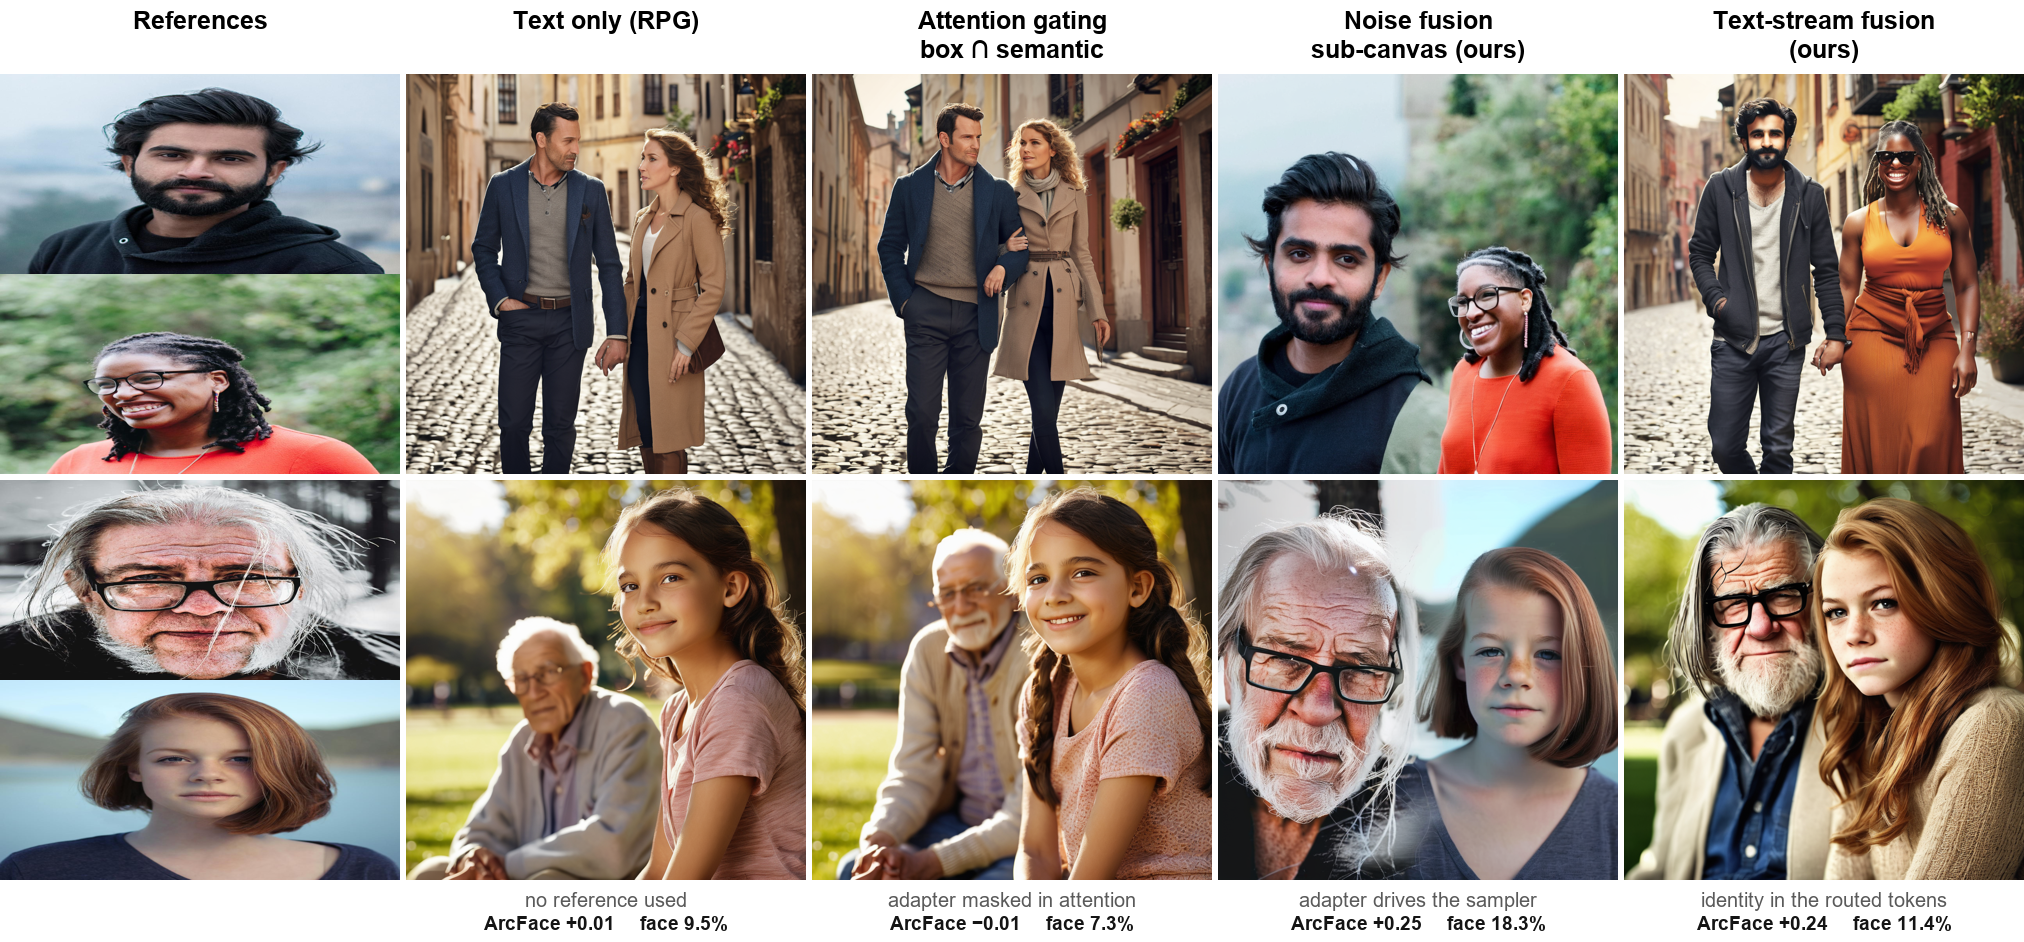
\includegraphics[width=\linewidth]{paper_figures/fig1_teaser.png}
  \caption{%
    \textbf{Where the reference enters decides what it costs.}
    Two references, one prompt, four places to put the identity, everything
    else held fixed.  \emph{Text only} composes the photograph the prompt
    asks for and contains neither reference person.  \emph{Attention gating}
    adds the adapter under the strongest mask the layout and the text
    attention can jointly produce---the planner's box intersected with the
    region's own semantic map---and the picture stays RPG's while the identity
    stays at chance: a mask says where identity may be written, not that there
    is any.  \emph{Noise fusion} lets the adapter drive the sampler instead,
    which delivers the identities and takes the composition with it, framing
    both subjects as busts.  \emph{Text-stream fusion} writes each identity
    into the class-noun token the planner already routes to that region, so
    nothing competes with the prompt for framing or pose.  ArcFace is measured
    on detected faces and does not move with framing; face area is the share of
    the canvas the faces occupy, against $9.5\%$ for the prompt's own medium
    framing.  Section~\ref{sec:framing} shows why the second number has to be
    reported beside the first.
  }
  \label{fig:teaser}
\end{figure*}

% ============================================================
\begin{abstract}
% ============================================================
Generating images that simultaneously portray \emph{multiple
specific concepts}—each guided by a user-provided reference
photograph—is a fundamental challenge in personalized image
synthesis.  Existing layout-guided methods (\eg, RPG) decompose
complex prompts into spatial regions and achieve strong
compositional correctness, but operate purely on text and cannot
preserve a concept's visual appearance.  Conversely, image-prompted
adapters (\eg, IP-Adapter) inject reference-image features globally,
causing \emph{cross-region leakage} in which one concept's appearance
bleeds into regions designated for another.

Training-free methods differ in \emph{where} they impose the spatial
constraint, and that choice is rarely isolated.  We hold the backbone,
the adapter, the injection scale, the layout planner and the seed fixed,
and vary only the injection site across three settings: masking the
adapter inside cross-attention, running a full per-region forward pass
and fusing at the noise level, and running that forward pass on a
per-region \emph{sub-canvas}.  The three form a ladder.  Attention-level
masking recovers $1.7\%$ of the identity gain the same adapter delivers from
the sampling loop, an amount indistinguishable from zero; whole-canvas noise
fusion recovers $68\%$; the sub-canvas formulation recovers all of it.  The gap between the first
two rungs is an order of magnitude and is not explained by injection
strength---driving the gated adapter to $2.5\times$ our own scale makes its
output move as far under a reference swap as ours does while its identity
response stays at zero---nor by the pipeline's base blending, which we sweep
to zero without effect.  The endpoint of the ladder is a complete method---an MLLM
planner assigns each reference to a region, IP-Adapter Plus encodes it,
and per-region sub-canvases are fused at the noise level with feathered
overlap in the spirit of
MultiDiffusion~\cite{bartal2023multidiffusion}---which we evaluate
against training-free and trained baselines alike.
This injects each reference's specific identity while structurally
containing it to the assigned region, suppressing the cross-region
leakage that global injection produces.
Because a purely regional trajectory never lets two concepts interact,
we further decouple identity from scene coherence \emph{in time}:
identity is committed during the early, high-noise steps, so the
regional decomposition can be released at a switch point $\tau$ and the
remaining steps taken on the full canvas, which resolves shared
lighting, background and perspective into a single scene.

On our proposed Mixed-Eval-v1 benchmark (150 two- and three-region
samples across person, object, and mixed categories), the endpoint of the
ladder is far above every training-free baseline---\textbf{DINO-ID
$0.720$} versus $0.352$ for RPG-only, ArcFace $0.266$ versus $0.129$, a
reference-specificity margin of $+0.247$ versus $+0.082$, and leakage
\textbf{Margin $+0.488$} versus $-0.082$ for global IP-Adapter---at
unchanged layout quality (\mbox{CLIP-T $0.645$}, matching RPG-only).
All of these are significant at $p{<}0.001$ under paired tests over the
same samples.
Similarity, however, cannot distinguish a weak adapter from a dead one, so we
add a control it cannot express: swap one region's reference for another
instance of the same category, hold everything else fixed, and ask whether the
output follows.  A reference-free baseline pins the change at exactly zero.
Under this test the gated adapter rewrites the image substantially yet moves
toward its newly assigned reference by an amount indistinguishable from zero
($p{=}0.79$), while every other conditioned method---ours included---moves at
$p{<}0.001$: attention-level injection perturbs the image without carrying the
particular identity it was handed.
Against MS-Diffusion---a multi-subject model trained on a
subject-annotated corpus, run here on the same backbone under a matched
protocol---we lead on identity, on placement and on isolation: DINO-ID
$0.720$ vs.\ $0.648$, ArcFace $0.266$ vs.\ $0.219$, and Margin $+0.488$ vs.\
$+0.437$ (all $p{<}0.001$), with the placement advantage widening from
$+0.031$ ($p{=}0.0001$) on three-region scenes.  It leads on text alignment
(CLIP-T $0.651$ vs.\ $0.647$, $p{=}0.005$), and recovers the isolation lead
when it is handed the non-adjacent layout of its own examples rather than our
planner's strips ($+0.439$ vs.\ $+0.420$, $p{=}0.024$), a sensitivity we
quantify.  Reaching that without its corpus, at $9.88$\,s per image against
$11.92$\,s, is what the injection site alone is worth.
Identity is near-flat in the release point $\tau$---DINO-ID varies by
$0.015$ over $\tau\in[0.5,1]$---so the late global phase is close to
free, and image realism improves with it (FID $136.3\!\to\!132.6$).
Swapping a region's reference mid-trajectory locates why: which subject a
region renders stops being reversible after step 6 of 30, so the release point
is set not by identity, which is settled a fifth of the way in, but by
isolation, which saturates far later.
No fine-tuning of the diffusion model is required.
\end{abstract}

% ============================================================
\section{Introduction}
\label{sec:intro}
% ============================================================

Text-to-image diffusion models have achieved remarkable synthesis
quality~\cite{rombach2022high,podell2024sdxl}, yet two complementary
limitations persist when users wish to generate images involving
\emph{multiple specific, pre-defined concepts}.

\textit{Layout-guided generation} methods such as
RPG~\cite{yang2024mastering} employ multimodal large language models
(MLLMs) to decompose a complex prompt into a structured spatial
plan—assigning sub-prompts to non-overlapping rectangular regions—
and synthesize each region with complementary regional diffusion
(CRD).  RPG achieves strong compositional correctness and spatial
arrangement, but operates purely on text: it cannot incorporate a
reference photograph to preserve a specific person's likeness.

\textit{Image-prompted generation} methods, most notably
IP-Adapter~\cite{ye2023ip}, inject visual features from a reference
image into the UNet's cross-attention layers via a lightweight
decoupled adapter.  IP-Adapter faithfully reflects the reference's
appearance in the output, but operates \emph{globally}: when multiple
reference images are provided, their features are uniformly mixed
across the entire image, causing \emph{cross-region leakage}—the
appearance of one concept bleeds into regions intended for a different
concept (Fig.~\ref{fig:teaser}).

\textbf{Conceptrol}~\cite{he2025conceptrol} addresses leakage by
deriving per-concept spatial masks from text cross-attention maps and
gating each concept's IP-Adapter features accordingly.  However,
Conceptrol lacks any scene planning capability and requires the token indices
of each concept to be specified in the prompt.  This is fragile for complex
multi-concept descriptions: its own token locator returns overlapping or
misplaced spans on 36 of our 150 benchmark prompts, because sibling regions
frequently repeat a head noun.  Supplying it with corrected spans, we find that
it does transfer identity, but merges the concepts into one subject rather than
placing them in separate regions (Margin $+0.004$; Section~\ref{sec:exp}).

We propose a method that unifies the strengths of all three
approaches.  Our key contributions are:

\begin{enumerate}

\item \textbf{The injection site, isolated by measurement.}
Training-free methods differ in where the spatial constraint is imposed, but
also in backbone, adapter, layout source and sampler, so the site itself has
never been isolated.  We hold all of the others fixed and vary only the site,
over four settings on the same $150$ samples and the same seed.  The identity
gain each recovers, as a share of what the same adapter delivers from the
sampling loop, is $1.7\%$, $65\%$, $68\%$ and $100\%$
(Fig.~\ref{fig:ladder}).  The first rung is the construction most
training-free work uses, and it is indistinguishable from zero
($p{=}0.35$); neither a larger injection strength nor the strongest mask the
site admits repairs it.  Section~\ref{sec:why_gating_fails} reports the
controls that close off the remaining explanations, including a cascade of
regional text attention with a semantic mask that delivers the pictures and
none of the identity.

\item \textbf{Sub-canvas regional compositing with a measured release point.}
We leave the adapter at full strength and move the constraint out of
attention: each planned region is denoised inside its own latent sub-canvas
by the unmodified adapter, and the per-region noise predictions are fused
with feathered overlap at every step.  Injection strength and spatial extent
are then governed by disjoint mechanisms, so identity and isolation stop
trading off.  Because a purely regional trajectory never lets two regions
interact, the partition is released at a switch point $\tau$.  We locate
$\tau$ by intervention rather than by sweeping it: replacing a region's
reference partway through the trajectory shows which subject the region
renders stops being reversible after step~$6$ of $30$, so the release point
is set by isolation rather than by identity (Section~\ref{sec:tau}).

\item \textbf{State of the art on identity and isolation, on instruments that
can establish it.}
On Mixed-Eval-v1 the method reaches the highest DINO-ID, leakage margin and
per-region face identity of every method we evaluate, ahead of
MS-Diffusion---trained on a subject-annotated corpus and run here on the same
backbone under a matched protocol---by $+0.072$, $+0.051$ and $+0.047$
respectively, all at $p{<}0.001$ and at $0.83\times$ its cost per image.  It
trails that baseline on text alignment by $0.004$, and we report the split
rather than a favourable subset.  Establishing this needs instruments the
literature lacks, which we contribute with it: identity specificity, which
separates reproducing \emph{the} reference from matching its category; a
reference-swap test, which asks whether the output depends on \emph{which}
reference was supplied and which a reference-free baseline pins at exactly
zero; and the observation that identity scores are read through framing
($r{=}0.949$ between face area and DINO-ID across seven methods), for which
we report a framing-independent measure alongside.  Mixed-Eval-v1 ($150$
samples) and Scaling-Bench ($90$) are released with the harness.

\end{enumerate}

\begin{figure*}[t]
  \centering
  \makebox[\linewidth][c]{%% One of the two drawn figures.  Colours and node styles are in
%% fig_tikz_defs.tex, input from the preamble of both builds.
%%
%% The four sites sit on ONE denoising step, which is the figure's argument:
%% they are alternatives at a single point in the computation, not four
%% different pipelines.  Drawing them as four separate diagrams would lose it.
%%
%% Site 4 deliberately has no bar.  The bars are a share of the identity gain
%% the sampling loop delivers; site 4 is scored by ArcFace on detected faces,
%% a different quantity, so a bar would put it on an axis it is not on.
%%
%% Alignment is held by construction rather than by hand: every column has an
%% x constant and a width, every row a y constant, and every box is centred on
%% its grid point at its column's width.  Changing a label cannot therefore
%% pull a box out of line with the one above it -- PROVIDED the width still
%% exceeds the label, which is why the widths below carry their contents'
%% measured size.  The whole drawing is 12.0cm against a 12.14cm text block.

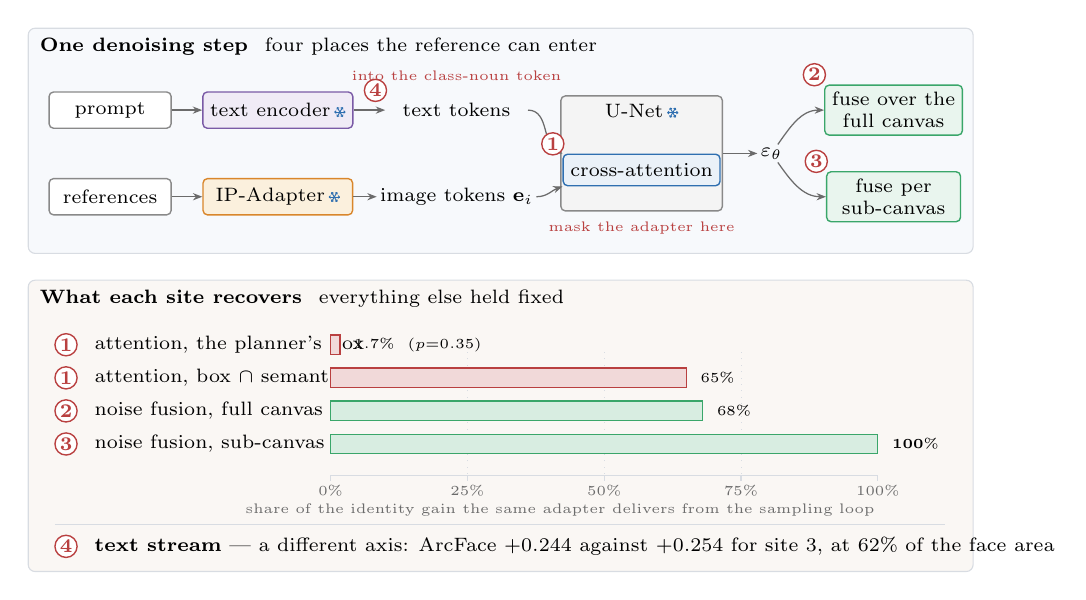
\begin{tikzpicture}[x=1cm,y=1cm]

  % ---- the grid -----------------------------------------------------------
  % widths are >= the measured width of the longest label in the column
  \def\xIn{0.90}    \def\wIn{1.55}     % inputs          (references: 1.19)
  \def\xEnc{3.03}   \def\wEnc{1.90}    % encoders        (text encoder: 1.58)
  \def\xTok{5.30}   \def\wTok{1.80}    % token streams   (image tokens: 1.61)
  \def\xNet{7.65}   \def\wNet{2.05}    % the U-Net       (cross-attn box: 1.82)
  \def\xEps{9.30}                      % the noise prediction
  \def\xFus{10.85}  \def\wFus{1.70}    % the two fusion sites (set two-line)
  \def\yTxt{2.02}   \def\yImg{0.92}    % the two conditioning streams
  \def\yNet{1.47}

  \def\bX{3.70}     % bars start here
  \def\bW{6.95}     % length of a 100% bar
  \def\bR{11.50}    % right edge of the panel's rules

  % ---- stage bands --------------------------------------------------------
  \fill[bandA,band] (-0.14,0.20) rectangle (11.86,3.06);
  \fill[bandB,band] (-0.14,-3.84) rectangle (11.86,-0.14);

  % ========================================================= one step ======
  \node[stage,anchor=north west] at (0.00,2.94)
    {One denoising step\ \ \textnormal{\scriptsize four places the reference
     can enter}};

  \node[blk,minimum width=\wIn cm,minimum height=0.46cm]  (pr) at (\xIn,\yTxt) {prompt};
  \node[blk,minimum width=\wIn cm,minimum height=0.46cm]  (rf) at (\xIn,\yImg) {references};
  \node[blkp,minimum width=\wEnc cm,minimum height=0.46cm](te) at (\xEnc,\yTxt) {text encoder\,\frozen};
  \node[blko,minimum width=\wEnc cm,minimum height=0.46cm](ie) at (\xEnc,\yImg) {IP-Adapter\,\frozen};
  \node[lbl,minimum width=\wTok cm] (tt) at (\xTok,\yTxt) {text tokens};
  \node[lbl,minimum width=\wTok cm] (it) at (\xTok,\yImg) {image tokens $\mathbf{e}_i$};

  \draw[ar] (pr) -- (te);   \draw[ar] (te) -- (tt);
  \draw[ar] (rf) -- (ie);   \draw[ar] (ie) -- (it);

  % the U-Net, with cross-attention called out inside it
  \node[blk,minimum width=\wNet cm,minimum height=1.46cm,fill=bgGrey]
    (unet) at (\xNet,\yNet) {};
  \node[lbl,anchor=north] at (\xNet,2.14) {U-Net\,\frozen};
  \node[blkb,minimum width=1.82cm,minimum height=0.40cm]
    (xa) at (\xNet,1.26) {cross-attention};
  \draw[ar] (tt) to[out=0,in=160] (xa.north west);
  \draw[ar] (it) to[out=0,in=200] (xa.south west);

  \node[lbl] (eps) at (\xEps,\yNet) {$\varepsilon_\theta$};
  \draw[ar] (unet) -- (eps);

  % two lines, so both boxes clear their text at one common width
  \node[blkg,minimum width=\wFus cm,minimum height=0.46cm]
    (fc) at (\xFus,\yTxt) {fuse over the\\full canvas};
  \node[blkg,minimum width=\wFus cm,minimum height=0.46cm]
    (sc) at (\xFus,\yImg) {fuse per\\sub-canvas};
  \draw[ar] (eps) to[out=55,in=180]  (fc.west);
  \draw[ar] (eps) to[out=-55,in=180] (sc.west);

  % ---- the four sites, each badged on the thing it names ------------------
  % one convention throughout: the badge sits just outside the north-west
  % corner of its target, so a reader finds them without hunting.
  \tikzset{badge/.style={site,xshift=-3.5pt,yshift=3.5pt}}
  \node[badge] (s4) at (tt.north west) {4};
  \node[badge] (s1) at (xa.north west) {1};
  \node[badge] (s2) at (fc.north west) {2};
  \node[badge] (s3) at (sc.north west) {3};

  \node[slbl,anchor=south,text=fgRed] at (\xTok,2.36)
    {into the class-noun token};
  \node[slbl,anchor=north,text=fgRed] at (\xNet,0.64)
    {mask the adapter here};

  % ========================================================= the ladder ====
  \node[stage,anchor=north west] at (0.00,-0.26)
    {What each site recovers\ \ \textnormal{\scriptsize everything else held
     fixed}};

  % a scale, so the bars are read against something
  \draw[rule,line width=0.4pt] (\bX,-2.62) -- (\bX+\bW,-2.62);
  \foreach \p in {0,25,50,75,100}{
    \draw[rule,line width=0.4pt] (\bX+\bW*\p/100,-2.62) -- ++(0,-0.07);
    \node[slbl,anchor=north,text=fgGrey] at (\bX+\bW*\p/100,-2.70) {\p\%};}
  \foreach \p in {25,50,75}{
    \draw[rule,line width=0.3pt,dotted] (\bX+\bW*\p/100,-2.60) -- ++(0,1.56);}

  \newcommand{\rung}[6]{%
    \node[site,fill=white] at (0.34,#1) {#2};
    \node[lbl,anchor=west] at (0.66,#1) {#3};
    \fill[#6!20,draw=#6,line width=0.45pt]
      (\bX,#1-0.125) rectangle (\bX+\bW*#4/100,#1+0.125);
    \node[slbl,anchor=west,text=black] at (\bX+\bW*#4/100+0.14,#1) {#5};}

  \rung{-0.96}{1}{attention, the planner's box}{1.7}{$1.7\%$\ \ ($p{=}0.35$)}{fgRed}
  \rung{-1.38}{1}{attention, box $\cap$ semantic}{65}{$65\%$}{fgRed}
  \rung{-1.80}{2}{noise fusion, full canvas}{68}{$68\%$}{fgGreen}
  \rung{-2.22}{3}{noise fusion, sub-canvas}{100}{$\mathbf{100\%}$}{fgGreen}

  \node[slbl,anchor=north east,text=fgGrey] at (\bX+\bW,-2.94)
    {share of the identity gain the same adapter delivers from the sampling
     loop};

  % site 4 is not on that axis and is given its own line rather than a bar
  \draw[rule,line width=0.4pt] (0.20,-3.24) -- (\bR,-3.24);
  \node[site,fill=white] at (0.34,-3.52) {4};
  \node[lbl,anchor=west,align=left] at (0.66,-3.52)
    {\textbf{text stream} --- a different axis: ArcFace $+0.244$ against
     $+0.254$ for site~3, at $62\%$ of the face area};

\end{tikzpicture}
}
  \caption{%
    \textbf{The four places a training-free method can put the reference.}
    All four are alternatives at a single denoising step, not four different
    pipelines.  The backbone, the adapter, the injection scale, the layout
    planner and the seed are held fixed across them; only the site varies.  Bars
    give the share of the identity gain the same adapter delivers from the
    sampling loop, so the ladder reads as a single quantity
    (Section~\ref{sec:why_gating_fails}).  Site~4 carries no bar because it is
    not on that axis: it writes identity into the class-noun token and is
    scored by ArcFace on detected faces (Section~\ref{sec:textstream}).
  }
  \label{fig:ladder}
\end{figure*}

We also report the boundaries of the result, since they are as informative as
the result: every number here is at $1024$, and at $768$ the comparison with
a trained model is far closer, for a reason we identify
(Section~\ref{sec:scaling}); the gating finding is established
on SDXL with IP-Adapter and a probe on a rectified-flow DiT suggests it may
not transfer (Section~\ref{sec:limitations}); and the panel structure that the
late release is meant to dissolve resists three separate repairs, for a reason
we can characterise but not remove (Section~\ref{sec:limitations}).

% ============================================================
\section{Related Work}
\label{sec:related}
% ============================================================

\noindent\textit{Text-to-Image Diffusion.}
Diffusion models~\cite{ho2020denoising} invert a fixed noising process;
deterministic samplers~\cite{song2021denoising,lu2022dpmsolver} and improved
schedules~\cite{karras2022elucidating} have reduced that inversion to a few
tens of network evaluations, which is what makes the inference-time
manipulation of the trajectory this paper relies on practical at all.  We
build on SDXL~\cite{podell2024sdxl}, a latent diffusion
model~\cite{rombach2022high}.

\noindent\textit{Layout-Guided Generation.}
GLIGEN~\cite{li2023gligen} grounds entities with gated self-attention over
boxes and tokens; BoxDiff~\cite{xie2023boxdiff} obtains the same control at
inference by energy-based guidance on attention maps.  Both belong to a family that manipulates
cross-attention, whose maps carry the layout~\cite{hertz2023prompt}.  Trained
layout controllers place instances more precisely still, at the cost of
layout-annotated training.  All of this work conditions each instance on
\emph{text}.
RPG~\cite{yang2024mastering} takes a complementary approach: it
uses GPT-4V to automatically decompose a complex prompt into a
structured spatial plan—assigning sub-prompts to non-overlapping
rectangular regions—and synthesizes each region with complementary
regional diffusion (CRD).  RPG achieves strong multi-concept layout
without fine-tuning, but operates purely on text and cannot preserve
a concept's \emph{visual} appearance.

\noindent\textit{Image-Prompted Personalization.}
DreamBooth~\cite{ruiz2023dreambooth} and Textual
Inversion~\cite{gal2022image} embed a concept by optimising weights or a
token embedding, which is impractical when references arrive only at
inference.  Training-free adapters address this: IP-Adapter~\cite{ye2023ip}
injects CLIP image features through decoupled cross-attention layers added to
a frozen backbone, its Plus variant replacing the pooled embedding with ViT
patch tokens and its FaceID variant adding
ArcFace~\cite{deng2019arcface} identity embeddings.
SSR-Encoder~\cite{zhang2024ssr} adds a token-to-patch aligner so only the
queried subject is encoded, and a further family trains on subject-annotated
corpora to transplant a reference into a scene.  Each encodes essentially \emph{one} concept per forward pass, which is where
the problem we study begins.

\noindent\textit{Multi-Concept Personalization.}
Several concepts at once is hard even with optimisation.  Custom
Diffusion~\cite{kumari2023multi} optimises embeddings jointly but bleeds
concepts at inference, and Mix-of-Show~\cite{gu2023mix} merges per-concept
LoRA~\cite{hu2022lora} adapters by gradient fusion, isolating better.  Both
optimise per concept.  LoRAShop~\cite{dalva2025lorashop} reaches the same conclusion we do about
\emph{where} the constraint belongs---it extracts a latent mask per concept
from the activations of a rectified-flow transformer and confines each LoRA to
that region rather than gating attention---but arrives at it from the opposite
end of the pipeline: its concepts must still be baked into LoRA weights
beforehand, so a reference photograph seen for the first time at test time
cannot be used.  We take the spatial constraint out of attention as well,
while keeping the adapter, and therefore the concept, free at inference.

\noindent\textit{Trained Multi-Subject Models.}
A second family removes the per-concept optimisation by \emph{training} a
multi-subject encoder.  FastComposer~\cite{xiao2024fastcomposer}
augments the text tokens with subject embeddings and adds a
cross-attention localisation loss, supervising each subject's attention
to concentrate on its own region---explicitly targeting the identity
blending we also measure.  MS-Diffusion~\cite{wang2025msdiffusion}
attaches grounding tokens and a layout-aware resampler to bind each
subject to a given box; XVerse~\cite{chen2025xverse} turns each reference
into a token-wise modulation offset inside a DiT, so subjects can be
controlled without touching the latents; MultiCrafter~\cite{wu2026multicrafter}
adds explicit positional supervision against attention bleeding, followed by
identity-aware preference alignment; and
$\lambda$-ECLIPSE~\cite{patel2024lambda} composes concepts in CLIP
latent space.  These results show that the binding problem is solvable
\emph{with} supervision: FastComposer learns the localisation that
training-free attention gating imposes analytically.  Our setting is the
training-free one---frozen backbone, frozen single-concept adapter, no
subject-annotated corpus---and our claim is correspondingly narrower:
\emph{absent} such training, the attention operator is the wrong site for
the constraint, and the sampling loop is a better one.
Section~\ref{sec:training_compare} sets out what the training-free
setting costs relative to trained multi-subject models.

\noindent\textit{Training-Free Multi-Concept Generation.}
Zero-shot approaches avoid optimisation entirely, and the dominant design is
to constrain each concept \emph{inside the attention layers}.
Conceptrol~\cite{he2025conceptrol} derives per-concept spatial masks
from text cross-attention maps and gates each concept's IP-Adapter
features to its mask.  It requires the token indices of each concept to be
specified, which is fragile for complex descriptions (Section~\ref{sec:conceptrol_setup}),
and lacks automated layout planning, so the per-region reference assignment
must also be provided manually.
More recent training-free work refines the same mechanism:
MC$^2$~\cite{mc2_2025} adds multi-concept guidance over the attention
maps, LaTexBlend~\cite{latexblend2025} blends concepts in a latent
textual space to scale to more subjects,
FreeCustom~\cite{freecustom2024} reuses self-attention features
across concepts, and AnyMS~\cite{yu2025anyms} performs bottom-up
dual-level attention decoupling---global decoupling of text and visual
conditions, plus local decoupling that confines each subject's
attention to its layout region.
AnyMS is the closest published setting to ours---training-free,
layout-guided, multi-subject, and built on the same backbone and adapter
family, SDXL with a pretrained IP-Adapter---so the measurement of
Section~\ref{sec:why_gating_fails} is scoped to the configuration the most
recent work in this line also occupies.  No public implementation was
available to us, and we do not substitute a reimplementation of our own;
Section~\ref{sec:why_gating_fails} places its local decoupling on our ladder
from its published description and states what our gated rows are and are
not.  What can be compared is the evaluation, and none of the axes this line
reports---layout control, reference similarity, text alignment---separates the
assigned reference from another instance of its category, or asks whether the
output depends on which reference was supplied.  Those are the two
measurements of Sections~\ref{sec:specificity} and~\ref{sec:refresponse}.

\noindent\textit{A third injection site: tokens.}
A newer line of training-free work bypasses attention entirely and edits
the denoising sequence itself.  Personalize
Anything~\cite{feng2026personalize} replaces denoising tokens with those
of a reference subject, aggressively early and with regularisation late,
and reports layout-guided multi-subject generation on a DiT;
FreeFuse~\cite{liu2025freefuse} routes between per-subject LoRAs at the
token level at test time.  This is a third answer to the question this
paper asks---the constraint can live in the attention operator, in the
sampling loop, or in the token sequence---and it is the one we do not
evaluate, because our study is built on a UNet backbone where the
token-replacement formulation does not directly apply.  We flag it as the
most important gap in the comparison.  Trained methods converge on the same
diagnosis from the other side:
PositionIC~\cite{hu2026positionic} attributes multi-subject failures to
``the entanglement of identity and layout by global attention
mechanisms'' and adds explicit spatial supervision to separate them, and
FocusDPO~\cite{jin2025focusdpo} applies preference optimisation to the
same class of errors.  These methods differ in \emph{how} the attention is
partitioned, but
share the assumption that spatial control belongs in the attention
operator.  Our measurements (Section~\ref{sec:why_gating_fails}) point to
a cost of that choice: injecting a reference through the masked path
alters the image substantially yet recovers no share of the identity gain
the same adapter delivers from the sampling loop that a paired test can
separate from zero, even when the injection is run at full strength, and
leaves face identity and identity specificity at the level of a text-only
baseline.  We keep the
adapter unmodified and impose the spatial constraint in the sampling loop
instead.

\noindent\textit{Identity-Preserving Generation.}
Single-face identity preservation has received significant attention.
PhotoMaker~\cite{li2024photomaker} stacks multiple reference-image ID
embeddings into the text token sequence, enabling zero-shot
multi-identity generation; however, it provides no explicit spatial
control to isolate each identity to a designated image region.
InstantID~\cite{wang2024instantid} combines IP-Adapter with a
ControlNet-based pose adapter and ArcFace embeddings for strong
single-face identity transfer, but is restricted to face concepts and
does not address multi-region scenes with heterogeneous concept types.

\noindent\textit{Region-Based Sampling.}
A separate line of work imposes spatial structure at the level of the
sampling trajectory rather than the attention operator.
MultiDiffusion~\cite{bartal2023multidiffusion} runs a shared diffusion
model over overlapping windows and fuses their predictions at each
step, originally to synthesise panoramas and region-conditioned scenes
from \emph{text}.  Its fusion rule is agnostic to what conditions each
window, which is precisely the property we exploit: we use it to carry
per-region \emph{image} conditioning, so that each concept is generated
by an untouched single-concept adapter and the spatial constraint is
expressed purely as geometry.

\noindent\textit{Positioning.}
Relative to attention-gated multi-concept methods
\cite{he2025conceptrol,mc2_2025,latexblend2025,freecustom2024,yu2025anyms},
our contribution is not another partitioning of the attention maps but
the observation that the partitioning site itself is the problem, plus
a compositing scheme that avoids it.  Relative to
MultiDiffusion~\cite{bartal2023multidiffusion}, we condition windows on
reference images rather than text, and show that the sub-canvas (rather
than full-canvas) formulation is what prevents centred subjects from
being merged into a single chimeric subject.  Relative to trained
multi-subject models~\cite{xiao2024fastcomposer,wang2025msdiffusion,ma2024subject},
we assume no subject-annotated training data and no layout supervision,
and so trade their fidelity for the ability to accept any concept, of any
category, that first appears at inference time.  Unlike Conceptrol, layout
planning and reference assignment are automated; unlike PhotoMaker and
InstantID, heterogeneous concept types are supported in arbitrary
multi-region layouts.

% ============================================================
\section{Method}
\label{sec:method}
% ============================================================

\begin{figure*}[t]
  \centering
  % 1.5cm wider than the review-mode text block, which cannot be recovered
  % without dropping the RPG-only panel the caption promises.  Centred, so the
  % bleed is 3.7mm into each 4.8cm margin rather than 7.4mm into one of them.
  \makebox[\linewidth][c]{%% One of the two drawn figures.  Colours and node styles are in
%% fig_tikz_defs.tex, input from the preamble of both builds.
%%
%% Laid out along the denoising timeline, because the contribution is a
%% timestep-level split: identity is written early inside per-region
%% sub-canvases, and the regional decomposition is released at tau.
%%
%% Planning is drawn out rather than shown as one box, after RPG's Figure 3:
%% the prompt's key phrases, the split ratio the planner emits, and the
%% per-region assignment are all visible, because the reference assignment is
%% the step that distinguishes this planner's output from a text-only one.
%% One colour per concept runs the whole width -- prompt phrase, region row,
%% sub-canvas, output label -- so a reader can follow one concept across the
%% figure without reading a single caption.
%%
%% The thumbnails are real renders.  There is deliberately no "the seam closes
%% at tau" before/after: measured over all 150 samples the release changes the
%% boundary step by at most 5%, which is not visible.
%%
%% Arrows attach to node anchors rather than to hardcoded coordinates, so a
%% box that grows with its text cannot silently overlap its neighbour.

\begin{tikzpicture}[x=1cm,y=1cm]

  % ---- stage bands, behind everything --------------------------------------
  \fill[bandA,band] (-0.14,-0.18) rectangle (6.52,3.60);
  \fill[bandB,band] (6.68,-0.18) rectangle (13.36,3.60);
  \fill[bandA,band] (-0.14,-3.30) rectangle (13.36,-0.42);

  % ======================================================== stage 1 =========
  \node[stage,anchor=north west] at (0.00,3.46) {Stage 1\ \ Scene planning};

  \node[blk,anchor=north west,text width=5.9cm,align=left,fill=white]
    (pr) at (0.00,3.06)
    {\emph{``\textcolor{fgBlue}{an elderly woman in a blue hoodie},
      {\scriptsize BREAK} \textcolor{fgGreen}{a potted plant on a stand}''}};

  \node[blkp,anchor=north west] (mllm) at (0.00,2.18)
    {MLLM planner\,\frozen};
  \node[slbl,anchor=west,align=left] at (1.92,2.02)
    {task instruction $+$ in-context\\examples $+$ chain of thought};

  % what the planner emits, drawn out -- this is the step a text-only planner
  % does not perform, so it is shown rather than summarised
  \node[blk,anchor=north west,text width=5.75cm,align=left,fill=white,
        inner sep=4pt,font=\tiny] (out) at (0.00,1.36)
    {split ratio \ \texttt{1,1}\\[1.5pt]
     \textcolor{fgBlue}{region 1 \ \ $p_1$: ``an elderly woman\ldots'' \ \
      ref $r_1$}\\[1.5pt]
     \textcolor{fgGreen}{region 2 \ \ $p_2$: ``a potted plant\ldots'' \ \ \
      ref $r_2$}};

  \draw[ar] (pr.south -| 0.72,0) -- (mllm.north -| 0.72,0);
  \draw[ar] (mllm.south -| 0.72,0) -- (out.north -| 0.72,0);

  % ======================================================== stage 2 =========
  \node[stage,anchor=north west] at (6.82,3.46)
    {Stage 2\ \ Reference encoding};

  % the references are consumed here, not in planning, so they are drawn here
  \node[thumb,draw=fgBlue,line width=0.6pt] (ra) at (7.44,2.56)
    {\includegraphics[width=0.60cm]{paper_figures/fg_ref_a.png}};
  \node[thumb,draw=fgGreen,line width=0.6pt] (rb) at (8.18,2.56)
    {\includegraphics[width=0.60cm]{paper_figures/fg_ref_b.png}};
  \node[slbl,anchor=north] at (7.81,2.18) {references $r_1$, $r_2$};

  \node[blko] (ipa) at (10.18,2.56) {IP-Adapter Plus\,\frozen};
  \node[lbl,anchor=west] (toks) at (11.68,2.56) {tokens $\mathbf{e}_i$};
  \draw[ar] (rb.east) -- (ipa.west);
  \draw[ar] (ipa.east) -- (toks.west);

  \node[slbl,anchor=north west,align=left,text width=6.3cm] at (6.84,1.70)
    {Each reference is encoded once, by the frozen encoder.  The adapter is
     never masked, attenuated or rescaled: Section~\ref{sec:why_gating_fails}
     shows that doing any of those is what stops identity arriving.};

  % ======================================================== stage 3 =========
  \node[stage,anchor=north west] at (0.00,-0.56)
    {Stage 3\ \ Sampling, split at $\tau$};

  % early
  \node[blkb] (u1) at (1.30,-1.36) {$\Omega_1$: U-Net\,\frozen $+\,\mathbf{e}_1$};
  \node[blkg] (u2) at (1.30,-2.30) {$\Omega_2$: U-Net\,\frozen $+\,\mathbf{e}_2$};
  \node[thumb,draw=fgBlue] (c1) at (3.28,-1.36)
    {\includegraphics[width=0.52cm]{paper_figures/fg_region1.png}};
  \node[thumb,draw=fgGreen] (c2) at (3.28,-2.30)
    {\includegraphics[width=0.52cm]{paper_figures/fg_region2.png}};
  \draw[ar] (u1.east) -- node[slbl,above,inner sep=1pt]{$\varepsilon_1$} (c1.west);
  \draw[ar] (u2.east) -- node[slbl,above,inner sep=1pt]{$\varepsilon_2$} (c2.west);

  \node[circle,draw=fgGrey,fill=white,inner sep=0pt,minimum size=10pt,
        font=\scriptsize,line width=0.5pt] (op) at (4.52,-1.83) {$\oplus$};
  \draw[ar] (c1.east) to[out=0,in=130] (op);
  \draw[ar] (c2.east) to[out=0,in=230] (op);
  \node[slbl,anchor=north,align=center] at (5.46,-1.76)
    {feathered\\fusion (Eq.~5)};

  \node[blk] (step) at (6.62,-1.83) {scheduler\\step};
  \draw[ar] (op) -- (step.west);
  \draw[ar,rounded corners=2pt] (step.north) -- ++(0,0.40) -| (u1.north);
  \node[slbl] at (4.20,-0.94) {repeat until $t=\tau$};

  \node[slbl,anchor=north west,align=left,text=black] at (0.00,-0.90)
    {\textbf{early} \ $t>\tau$};

  % the switch
  \draw[fgRed,dashed,line width=0.55pt] (7.46,-3.22) -- (7.46,-0.60);

  % late
  \node[slbl,anchor=north west,align=left,text=black] at (7.62,-0.90)
    {\textbf{late} \ $t\le\tau$};
  \node[blkr] (u3) at (9.22,-1.83)
    {U-Net\,\frozen, full canvas\\$+\,p,\ \{\mathbf{e}_i\}$};
  \draw[ar] (step.east) -- (u3.west);

  \node[thumb] (fin) at (11.52,-1.83)
    {\includegraphics[width=0.92cm]{paper_figures/fg_ours.png}};
  \draw[arh] (u3.east) -- (fin.west);
  \node[slbl,anchor=north,align=center] at (11.52,-2.38)
    {\textcolor{fgBlue}{region 1} and \textcolor{fgGreen}{region 2},\\each its
     own reference};

  \draw[rule,line width=0.4pt] (12.36,-2.52) -- (12.36,-1.16);
  \node[thumb,draw=fgGrey!45] (rpg) at (12.92,-1.83)
    {\includegraphics[width=0.58cm]{paper_figures/fg_rpgonly.png}};
  \node[slbl,anchor=north,align=center] at (12.92,-2.20) {text only:\\neither};

  % timeline
  \draw[arh] (0.00,-3.52) -- (13.30,-3.52);
  \node[slbl,anchor=north west] at (0.00,-3.60) {$t=T$ \ (noise)};
  \node[slbl,anchor=north east] at (13.30,-3.60) {$t=0$ \ (image)};
  \draw[fgRed,line width=0.55pt] (7.46,-3.66) -- (7.46,-3.38);
  \node[slbl,anchor=north,text=fgRed] at (7.46,-3.66) {$\tau$ \ (default $0.7$)};

\end{tikzpicture}
}
  \caption{%
    \textbf{The endpoint of the ladder as a complete method.}
    An MLLM planner assigns each reference to a region and IP-Adapter Plus
    encodes it; sampling then splits at one switch point $\tau$.
    \emph{Early} ($t>\tau$), each region is denoised inside its own latent
    sub-canvas $\Omega_i$ by the \emph{unmodified}, full-strength adapter, and
    the per-region noise predictions are fused with feathered overlap
    (Eq.~\ref{eq:fuse}) before a single scheduler step.
    \emph{Late} ($t\le\tau$), sampling switches to one full-canvas pass on the
    global prompt and all $\mathbf{e}_i$, which is where the regions can in
    principle resolve into a shared scene; Section~\ref{sec:limitations}
    reports how far that goes, and it is less far than the design intends.
    Snowflakes mark frozen modules---every module here is frozen---and the
    adapter is never masked or rescaled, so spatial control comes from the
    sub-canvas geometry alone.  The thumbnails are renders, not illustrations:
    the two references, the two halves of our own output, and RPG-only on the
    same prompt and seed.
  }
  \label{fig:method}
\end{figure*}

\subsection{Overview}
\label{sec:overview}

The input is a text description $\mathcal{P}$ naming $N$ concepts, together
with one reference photograph $r_i$ per concept, supplied at inference time.
The output is a single image in which concept $i$ occupies its own spatial
region, carries the appearance of $r_i$ rather than of a generic member of
its category, and does not contaminate the regions assigned to the other
concepts.  No per-concept optimisation is permitted: the references are first
seen when the image is requested.

Fig.~\ref{fig:method} shows the four stages.  \emph{Scene planning}
(Section~\ref{sec:planning}) turns $\mathcal{P}$ into a partition of the
canvas, a sub-prompt per region, and---the step that distinguishes this
planner's output from RPG's---an assignment of each reference to a region.
\emph{Image feature encoding} (Section~\ref{sec:encoding}) maps each $r_i$ to
visual tokens $\mathbf{e}_i$ through the frozen IP-Adapter Plus encoder.
\emph{Early sampling} (Section~\ref{sec:subcanvas}) denoises every region
inside its own latent sub-canvas with the unmodified adapter at full
strength, fusing the per-region noise predictions with feathered overlap
before each scheduler step.  \emph{Late sampling} (Section~\ref{sec:tau})
releases the partition at a switch point $\tau$ and takes the remaining steps
on the full canvas.

Every module is frozen.  The diffusion backbone, the text encoders, the image
encoder and the adapter's projection layers are used exactly as released; the
method adds no parameters and performs no fine-tuning, and its only
hyper-parameters are the injection scale $\lambda$, the sub-canvas overlap
$o$ and the switch point $\tau$.  The adapter in particular is never masked,
attenuated or rescaled---a decision that is the subject of
Section~\ref{sec:why_gating_fails}, where we show that doing any of those
things is what prevents identity from arriving in the first place.

Throughout, $i$ indexes regions, $t$ indexes the $T$ denoising steps counted
down from noise to image, $\Omega_i$ denotes region $i$'s latent sub-canvas,
and $\varepsilon_\theta$ is the frozen noise predictor.

\subsection{MLLM Scene Planning}
\label{sec:planning}

A multimodal large language model is used because the partition has to follow
from the sentence rather than from the image: at planning time no image
exists, so the number of regions, their relative extents and which concept
belongs in each must be read out of the prompt's syntax and its implied
composition.  We follow RPG~\cite{yang2024mastering} in both the prompting
scheme and the representation, and add the reference assignment.

\noindent\textit{Prompt structure.}
GPT-4V is given a fixed template followed by the user prompt.  The template
has three parts: a task instruction establishing the model's role as a region
planner and the output format; a small set of in-context examples pairing a
complex prompt with its decomposition; and a chain-of-thought trigger that
makes the model state the composition it is reasoning toward before emitting
the partition.  The examples are chosen to carry two rules that the format
alone does not express---objects sharing a class name take separate regions,
so that counts are preserved, and attribute phrases stay attached to the
subject they modify rather than being split across regions.

\noindent\textit{Representation.}
The planner emits a \emph{split ratio} and one sub-prompt per region.  The
split ratio is a string in which \texttt{;} separates rows and \texttt{,}
separates columns within a row, each number giving that element's extent
relative to its siblings; \texttt{1,1} is therefore two equal columns and
\texttt{1;2,1} a short top row above a bottom row split two-to-one.  Parsing
it yields the rectangles
\begin{equation}
  \bigl\{(b_i,\, p_i,\, \mathrm{ref}{=}i)\bigr\}_{i=1}^{N},
  \qquad b_i=(x_0,y_0,x_1,y_1)\in[0,1]^4 ,
\end{equation}
where $b_i$ is a normalised box and $p_i$ the sub-prompt for region $i$.  The
rectangles tile the canvas and do not overlap, which is what makes the
sub-canvas construction of Section~\ref{sec:subcanvas} well defined and is
also, as Section~\ref{sec:limitations} reports, the source of two of the
method's costs.

\noindent\textit{Reference assignment.}
The third field is the one the personalisation setting requires and that a
text-only planner does not produce: the planner binds the $i$-th reference
photograph to the $i$-th region, in the same pass that writes the sub-prompt.
The binding is available because the planner has already decided which
concept each region contains, so naming the reference costs nothing extra.
This replaces the manual annotation that attention-gated methods need:
Conceptrol~\cite{he2025conceptrol} requires the token indices of each
concept to be supplied by hand, and those indices are fragile when a prompt
repeats a head noun, which the person and mixed splits of our benchmark
routinely do (Section~\ref{sec:conceptrol_setup}).

Planning is one API call per prompt and is excluded from the per-image
timings of Section~\ref{sec:efficiency}, since it is paid once per layout rather
than once per image; its cost and latency are a dependency we record in
Section~\ref{sec:limitations}.

\subsection{Image Feature Encoding}
\label{sec:encoding}

Each reference $r_i$ is encoded by the IP-Adapter Plus image encoder
(CLIP ViT-H/14):
\begin{equation}
  \mathbf{e}_i = \mathrm{ImageEncoder}(r_i)\in\mathbb{R}^{257\times 1280}.
\end{equation}
These are projected into key-value pairs for UNet injection via
IP-Adapter's learned linear layers $W_K^{\mathrm{IP}},
W_V^{\mathrm{IP}}$.

\subsection{What Attention-Level Gating Writes}
\label{sec:why_gating_fails}

The natural way to make IP-Adapter regional is to gate its features
inside the cross-attention layers: compute an IP branch per concept and
mask it to that concept's region before adding it to the text branch,
\begin{equation}
  \mathbf{h}' = \mathbf{h}^{\mathrm{text}}
    + \lambda \sum_{i=1}^{N}\mathbf{m}_i \odot
      \operatorname{Attn}\!\bigl(\mathbf{Q},\,W_K^{\mathrm{IP}}\mathbf{e}_i,\,
      W_V^{\mathrm{IP}}\mathbf{e}_i\bigr),
  \label{eq:gated}
\end{equation}
which is the formulation underlying
Conceptrol~\cite{he2025conceptrol} and related regional adapters.

Eq.~\ref{eq:gated} is appealing, but in our experiments it fails to
deliver instance identity even when nothing attenuates it.  We run it at
the same full scale $\lambda$ used by our own method, with the residual
unmasked, no per-layer rescaling, and no restriction of the injection to
a subset of denoising steps.  So configured, the adapter is
unambiguously active: not one of the 150 outputs coincides with the
text-only regional baseline, and the mean absolute pixel difference from
that baseline is $5.6\times$ larger than for an attenuated
configuration, while prompt adherence is if anything slightly improved
(CLIP-T $0.652$ vs.\ $0.650$).

What the injection adds, however, is mostly not the assigned reference.
Per-region identity moves from DINO-ID $0.352$ to $0.358$, a difference a
paired test cannot separate from zero ($p{=}0.35$); only Margin moves
detectably, $+0.076$ to $+0.098$ ($p{=}0.004$).  Both are an order of
magnitude short of the $+0.368$ and $+0.412$ the same adapter delivers from
the sampling loop.  Face identity (ArcFace $0.129\!\to\!0.122$) and identity
specificity (Section~\ref{sec:specificity}, $0.082\!\to\!0.089$) do not move
either.  The
adapter fires at full strength and writes appearance belonging largely to
each concept's \emph{category} rather than to its \emph{instance}.  Driving
$\lambda$ to $2.5\times$ does not change this
(Section~\ref{sec:refresponse}).  We report
this as an empirical property of the injection site: we do not claim to
have isolated the mechanism responsible for it.
Section~\ref{sec:exp} quantifies the effect, and
Section~\ref{sec:subcanvas} shows that relocating the identical adapter,
at the identical scale, into the sampling loop raises specificity to
$0.215$.

\subsection{Sub-Canvas Regional Compositing}
\label{sec:subcanvas}

We therefore leave the adapter untouched and move the spatial
constraint from attention into the sampling loop.  Let
$\mathbf{z}_t\in\mathbb{R}^{C\times h\times w}$ be the latent at step
$t$.  Each planned box $b_i$ maps to a latent sub-window
$\Omega_i=[u_i,u_i')\times[v_i,v_i')$, dilated by an overlap of $o$
latent columns on interior sides so that neighbouring regions share a
transition band (Fig.~\ref{fig:masks}).  Write $\mathcal{C}_i$ for
cropping to $\Omega_i$ and $\mathcal{C}_i^{\!\top}$ for pasting back.

\noindent\textit{Per-region prediction.}  Each region is denoised as an
independent image of its own size, using the \emph{standard} adapter at
full scale $\lambda$ with that region's sub-prompt $p_i$ and reference
embedding $\mathbf{e}_i$:
\begin{equation}
  \boldsymbol{\epsilon}_i =
    \epsilon_\theta\!\bigl(\mathcal{C}_i(\mathbf{z}_t),\,t,\,p_i,\,
    \mathbf{e}_i;\,\lambda\bigr),
  \label{eq:region_eps}
\end{equation}
with classifier-free guidance applied inside $\epsilon_\theta$.  No
masking or rescaling touches the adapter, so the identity signal in
$\boldsymbol{\epsilon}_i$ is exactly that of single-concept
IP-Adapter generation.

\noindent\textit{Noise-level fusion.}  The regional predictions are
merged on the full canvas with feathered weights $\mathbf{w}_i$, which
ramp linearly from $0$ to $1$ across the overlap band and are $1$
elsewhere in $\Omega_i$:
\begin{equation}
  \boldsymbol{\epsilon} =
  \frac{\sum_{i=1}^{N}\mathcal{C}_i^{\!\top}
        \bigl(\mathbf{w}_i\odot\boldsymbol{\epsilon}_i\bigr)}
       {\sum_{i=1}^{N}\mathcal{C}_i^{\!\top}(\mathbf{w}_i)},
  \qquad
  \mathbf{z}_{t-1}=\operatorname{Step}(\boldsymbol{\epsilon},t,\mathbf{z}_t).
  \label{eq:fuse}
\end{equation}
A single scheduler step is taken on the fused prediction, so all
regions stay on one shared denoising trajectory and inherit a common
global structure rather than being stitched post hoc.

\noindent\textbf{Why sub-canvases and not the full canvas.}
A simpler variant runs Eq.~\ref{eq:region_eps} on the \emph{whole}
canvas per concept and relies on $\mathbf{w}_i$ alone to separate them.
This fails for centred subjects: each pass independently places its
subject in the middle of the frame, and the masks then cut two halves
of two different subjects and glue them together---producing a single
chimeric subject rather than two.  Denoising inside $\Omega_i$ forces
each subject to be composed \emph{within} its own region, which removes
the failure mode entirely (Table~\ref{tab:ablation},
Fig.~\ref{fig:ablation_vis}).

\noindent\textbf{Relation to prior formulations.}
With $N{=}1$ and $\Omega_1$ the full canvas, Eq.~\ref{eq:fuse} reduces
exactly to standard IP-Adapter sampling.  The fusion rule is that of
MultiDiffusion~\cite{bartal2023multidiffusion}, here used to carry
\emph{per-region image conditioning} rather than text panoramas.
Unlike Eq.~\ref{eq:gated}, injection strength and spatial extent are
controlled by two disjoint mechanisms---$\lambda$ and $\Omega_i$---so
tightening isolation no longer weakens identity.

\subsection{Late Global Release}
\label{sec:late_release}

Sub-canvas compositing solves identity, but it also creates a problem of
its own.  Because every region is denoised as an independent image for
the entire trajectory, no computation ever sees two regions at once: the
subjects are assembled side by side without shared lighting, ground
plane, background or perspective, and the result reads as a set of
pasted panels rather than one photograph.  This is a structural
consequence of the geometry, not a tuning failure---no choice of
$\lambda$ or $o$ can remove it.

Our remedy exploits a well-known property of diffusion sampling: the
early, high-noise steps fix layout and identity, while the late,
low-noise steps refine appearance and global consistency.  Identity and
coherence therefore need not be produced by the same mechanism at the
same time.  We introduce a single switch point $\tau\in[0,1]$ and split
the trajectory in two.  For the first $\tau$ fraction of steps we sample
with Eqs.~\ref{eq:region_eps}--\ref{eq:fuse} as above.  For the
remaining steps we discard the regional decomposition entirely and take
one \emph{full-canvas} pass per step,
\begin{equation}
  \boldsymbol{\epsilon} =
    \epsilon_\theta\!\bigl(\mathbf{z}_t,\,t,\,\mathcal{P},\,
    \{\mathbf{e}_i\};\,\lambda\bigr),
  \label{eq:release}
\end{equation}
conditioned on the \emph{global} prompt $\mathcal{P}$ and the pooled
reference embeddings.  Because the regional phase has already committed
each subject's identity and position into $\mathbf{z}_t$, the global
phase cannot relocate or overwrite them; it can only reconcile what they
share---illumination, shadows, contact with the ground, and the
background that runs behind both.

$\tau{=}1$ recovers pure sub-canvas compositing, and $\tau{=}0$ is
ordinary global IP-Adapter sampling with no regional control at all.
The interesting behaviour is in between, and it is markedly asymmetric:
Section~\ref{sec:tau} shows that identity survives almost unchanged down to
$\tau\!\approx\!0.5$, so a substantial released phase is available at
essentially no cost in identity.  Whether that phase delivers the scene
coherence it exists for is a separate question, and one we were unable to
measure (Section~\ref{sec:limitations}).
The premise that the regional phase has already committed identity is not
assumed here but measured: swapping a region's reference mid-trajectory stops
changing which subject is rendered after step 6 of 30
(Section~\ref{sec:commitment}), a fifth of the way through, so the release at
$\tau{=}0.7$ happens well after the choice of subject is closed.

\subsection{Implementation}
\label{sec:method_impl}

Regions are denoised sequentially within each step, so peak memory is
that of a single sub-canvas forward pass and is independent of $N$;
the whole pipeline runs on one 16\,GB GPU.  We use $\lambda=0.8$, an
overlap of $o=8$ latent columns and a release point $\tau=0.7$
throughout, and take a single DPM-Solver++ step per fused prediction.
No component of the diffusion model, the adapter, or the text encoders
is fine-tuned.

% ============================================================
\section{Experiments}
\label{sec:exp}
% ============================================================

\subsection{Setup}

\noindent\textit{Dataset.}
We construct \emph{Mixed-Eval-v1}, a benchmark of 150 samples across
three categories: \emph{person} (50, two-region portraits),
\emph{object} (50, two-region product compositions), and \emph{mixed}
(50, two/three-region scenes).  Each sample provides a global prompt,
per-region sub-prompts, a split-ratio string, and \textbf{two}
reference images per region (ref-A for guidance; ref-B for
multi-reference identity scoring).
Sub-prompts draw a subject and two attributes from fixed lists, and we record
a defect of that construction: nothing prevents both attributes coming from
the same group, so $20$ of the $179$ person sub-prompts ($11.2\%$) contradict
themselves---``a teenage girl, with long black hair, with short blonde hair''.
Every method receives the identical prompt, so this adds noise to absolute
scores rather than bias to comparisons, and identity is scored against the
reference photographs rather than the prompt; it does depress text alignment
on the affected samples.  A revision should sample attributes from distinct
groups.
Two derived sets carry measurements Mixed-Eval-v1 cannot support on its own.
\emph{Scaling-Bench} extends the same task past three regions---90 samples,
30 each at $N{=}4,5,6$, drawn from the same reference pool and balanced
across the three categories (Section~\ref{sec:scaling}).  The
\emph{reference-swap twin} is a 30-sample subset in which region~0's
reference is exchanged for a different instance of the same category with
prompt, layout, seed and the remaining reference held fixed
(Section~\ref{sec:refresponse}).

\noindent\textit{Implementation.}
We use SDXL-base-1.0~\cite{podell2024sdxl} with
DPM-Solver++~\cite{lu2022dpmsolver} on the Karras sigma
schedule~\cite{karras2022elucidating}
(30 steps, CFG\,=\,7.5), IP-Adapter Plus ViT-H weights from
\texttt{h94/IP-Adapter} (SDXL variant, \texttt{ip-adapter-plus\_sdxl\_vit-h}),
full injection scale $\lambda=0.8$, sub-canvas overlap $o=8$ latent columns,
seed 42, and resolution $1024\!\times\!1024$ throughout---SDXL's native
training resolution, and the same for every method.  The choice is not
neutral: an earlier version evaluated at $768$, where the two methods respond
to resolution in opposite directions (Section~\ref{sec:limitations}).  Peak
memory is $15.8$\,GB, which fits a $16$\,GB card with little margin.  No
fine-tuning is performed.

\noindent\textit{Baselines.}
\begin{itemize}\setlength\itemsep{2pt}
\item \textbf{RPG-only}: regional diffusion with text sub-prompts
      only; no reference image.
\item \textbf{IP-Adapter (global)}: applied globally with the first
      reference and no regional assignment, at the same $\lambda{=}0.8$
      through the same pipeline and weights, so the two differ only in
      whether the spatial decomposition is present.
\item \textbf{Conceptrol}$^{\dagger}$~\cite{he2025conceptrol}: per-concept
      spatial gating via text cross-attention masks, run from the authors'
      official code (Section~\ref{sec:conceptrol_setup}).
\item \textbf{MS-Diffusion}$^{\P}$~\cite{wang2025msdiffusion}: grounding
      tokens plus a layout-aware resampler, trained once on a
      subject-annotated corpus and applied zero-shot.  It is the closest
      published comparison---same backbone, no per-concept optimisation,
      references and boxes supplied at inference---and is run from the
      authors' code and checkpoint.
\end{itemize}

%%SUPP{conceptrol_cfg}
\noindent\textit{Conceptrol setup.}
\label{sec:conceptrol_setup}
We use the authors' \texttt{Conceptrol\allowbreak IPAdapter\allowbreak Plus\allowbreak XL} unmodified, on the same
SDXL-base-1.0 backbone and the same \texttt{ip-adapter-plus\_sdxl\_vit-h}
weights as our method ($16$ image tokens), at $768\!\times\!768$, 30
DPM-Solver++ steps, CFG 7.5, seed 42.  Conceptrol derives its concept masks
from text cross-attention and has no layout planner, so it receives the global
prompt and the same per-region references; this is its intended usage.  We make
one change, which favours the baseline.  Its helper locates a concept's tokens
with \texttt{tokens.index(subject\_tokens[0])}, i.e.\ the \emph{first}
occurrence, which returns overlapping or misplaced spans on 36 of our 150
prompts---the person and mixed splits routinely repeat a head noun (``a teenage
girl \ldots\ a teenage girl'').  We replace it with an ordered subsequence
search that advances a cursor past each match, giving disjoint, correctly
placed spans on all 150 prompts.  Conceptrol therefore receives better concept
indices than its own helper produces.  We also swept the injection scale over
$\{0.8, 1.0\}$ across the full benchmark and report the stronger result.
%%ENDSUPP

%%SUPP{msdiff_cfg}
\noindent\textit{MS-Diffusion setup.}
\label{sec:msdiffusion_setup}
We run the authors' released code and \texttt{ms\_adapter.bin} on
SDXL-base-1.0 with the CLIP-G image encoder they specify, at
$768\!\times\!768$, 30 DPM-Solver++ steps, CFG 7.5, seed 42 and our negative
prompt, so the two methods differ in mechanism rather than in sampling
configuration.  Each planned region is passed as one normalised box and the
head noun phrase of its sub-prompt as the matching phrase.  Two details
favour the baseline.  Its span helper matches on whitespace-split words and
strips trailing punctuation on the prompt side only, so a phrase carrying an
internal comma silently resolves to the empty span $[0,0]$ and the layout
guidance is disabled; we verified on all 150 prompts that the phrases we pass
resolve to non-empty, mutually disjoint spans.  Adjacent full-height boxes
also leave no background region, so we additionally ran the tighter,
non-adjacent box shape used in the authors' own examples, and report the
stronger of the two.  As with the other baselines, the injection scale was
swept and the better setting reported.
%%ENDSUPP

\noindent\textit{Significance testing.}
\label{sec:significance}
Every variant is generated from the same 150 samples under the same seed, so
all comparisons are paired.  We report the paired mean difference with a
95\% confidence interval, a two-sided $t$ test, and a Wilcoxon signed-rank
test as a distribution-free check; the two agree on every comparison in this
paper except one, noted where it arises.  We flag a comparison as a tie when
neither test rejects at $p{<}0.05$, and we do so even when the point estimate
favours us---which it does at $N{=}2$ on binding accuracy, and on identity
specificity, both against MS-Diffusion.  The distinction matters most in that
comparison, where the differences are an order of magnitude smaller than
against the training-free baselines: our $2.0\times$ gain in DINO-ID over a
text-only baseline is significant at $p{<}0.001$ on 149 of 150 samples, while
the same metric against MS-Diffusion is a $+0.072$ difference at
$p{<}0.001$, while binding accuracy against the same baseline is $+0.019$ at
$p{=}0.17$ and is reported as the tie it is.

\noindent\textit{Ablations.}
\begin{itemize}\setlength\itemsep{2pt}
\item \textbf{Attention gating}: the adapter of Eq.~\ref{eq:gated} masked to
      each region \emph{inside} cross-attention, evaluated both attenuated for
      leakage suppression and at full strength ($\lambda{=}0.8$, no per-layer
      or per-timestep gating).
\item \textbf{Noise fusion, full-canvas}: our fusion rule
      (Eq.~\ref{eq:fuse}) but with each concept denoised over the whole
      canvas instead of its sub-window.
\end{itemize}

\noindent\textit{Metrics.}
\begin{itemize}\setlength\itemsep{2pt}
\item \textbf{DINO-ID}$\uparrow$: DINOv2-base~\cite{oquab2024dinov2}
      cosine similarity between ref-A and the corresponding region crop.
\item \textbf{Margin}$\uparrow$:
      $\mathrm{DINO\text{-}ID}(r_i,\mathrm{crop}_i)
       -\max_{j\neq i}\mathrm{DINO\text{-}ID}(r_j,\mathrm{crop}_i)$.
      Positive = concept isolation; negative = leakage.
\item \textbf{CLIP-T}$\uparrow$: CLIP ViT-L/14~\cite{radford2021learning}
      image–text cosine similarity (full image vs.\ global prompt).
\item \textbf{ArcFace}$\uparrow$: ArcFace~\cite{deng2019arcface}
      (buffalo\_l) face embedding
      cosine similarity; reported on samples with detected faces
      (${\approx}68\%$ detection rate).
\item \textbf{Binding accuracy}$\uparrow$: fraction of regions whose crop
      matches its own regional sub-prompt better than any sibling
      sub-prompt, under CLIP.  Threshold-free, internal to one image, with
      chance at $1/N$ (Section~\ref{sec:binding}).
\item \textbf{Reference response} ($S$, $D$): with one region's reference
      swapped for a same-category instance and everything else fixed, $S$ is
      how far the output moves and $D$ how much of that movement is
      \emph{toward} the newly assigned reference.  Unlike the similarity
      metrics above, this one has a known correct value for a
      reference-free method---$S{=}0$ (Section~\ref{sec:refresponse}).
\item \textbf{FID}$\downarrow$~\cite{heusel2017gans} and
      \textbf{KID}$\downarrow$~\cite{binkowski2018demystifying}
      ($\times 10^{3}$): computed with clean-fid against the 750
      Mixed-Eval-v1 reference photographs.  FID's Gaussian estimator is
      strongly biased at $150$ samples, so we report the unbiased kernel
      estimator beside it.  Neither is a criterion for this task---the
      reference photographs are single-subject and the task is
      multi-subject---and we use them only to check that outputs are not
      degenerate (Section~\ref{sec:exp}).
\end{itemize}

% ---- Table 1 ----------------------------------------------------------------
\subsection{Main Results}
\label{sec:main_results}

Table~\ref{tab:main} compares our method against the training-free
baselines on all 150 Mixed-Eval-v1 samples; the analysis that follows
reads it row by row, and Fig.~\ref{fig:metrics_chart} visualises the
leakage-margin and per-category identity gaps.

\begin{table}[htbp]
\centering
\caption{%
  \textbf{Comparison on Mixed-Eval-v1} (150 samples, all categories, every
  method at $1024\!\times\!1024$).
  Our proposed methods \textbf{highlighted in bold}.
  ArcFace-P: person category only.
  FID and KID ($\times 10^{3}$) computed with clean-fid against the 750
  Mixed-Eval-v1 reference photographs.  Both are reported for completeness
  and neither is a criterion here: the reference set consists of
  \emph{single-subject} photographs while every method is asked to produce a
  \emph{multi-subject} scene, so both metrics reward failing the task
  (see text).  Ours is not bolded on them.
  Every difference between Ours and a baseline on DINO-ID and Margin is
  significant at $p{<}0.001$ under a paired test over the same 150 samples,
  including against MS-Diffusion ($+0.072$ and $+0.051$).  On CLIP-T the
  ordering runs the other way: MS-Diffusion leads us by $0.004$ ($p{=}0.005$)
  and RPG-only by $0.005$ ($p{=}0.009$), because conditioning a region on a
  reference pulls it away from the generic rendering a prompt alone produces
  (Section~\ref{sec:limitations}).
  Attention gating is the full-strength ablation of
  Section~\ref{sec:why_gating_fails}, listed here because the row a reader
  should compare it against is RPG-only directly above it: it rewrites every
  image and lands on the text-only baseline
  (Section~\ref{sec:significance}).
  $\dagger$: Conceptrol~\cite{he2025conceptrol}, run from the authors'
  official implementation (\texttt{Conceptrol\allowbreak IPAdapter\allowbreak Plus\allowbreak XL}) with the same
  SDXL backbone, IP-Adapter Plus ViT-H weights, resolution, scheduler, steps,
  CFG and seed as ours.  Injection scales $1.0$ (the authors' default) and
  $0.8$ (matched to our $\lambda$) were both run over all 150 samples and the
  stronger of the two ($0.8$) is reported; at $1.0$ the row reads
  $0.357/{+}0.004/0.621/0.155/0.153/130.8/26.8$.  Conceptrol has no layout planner,
  so it receives the global prompt, and we supply corrected per-concept token
  spans (Section~\ref{sec:conceptrol_setup}).
  $\P$: MS-Diffusion~\cite{wang2025msdiffusion}, run from the authors'
  released code and \texttt{ms\_adapter.bin} on the same SDXL-base-1.0
  backbone, at the same resolution, scheduler, steps, CFG and seed as ours,
  and driven by our planner's regions.  Four configurations were run over the
  full benchmark---injection scale $\{0.6$ (the authors' default), $0.8$
  (matched to our $\lambda)\}$ crossed with box shape $\{$our adjacent
  full-height strips, the tighter non-adjacent shape used in the authors'
  examples$\}$---and the strongest is reported (scale $0.8$, tight boxes).
  The box shape matters more than the scale: with our strips the same scale
  reads $0.509/{+}0.327/0.645/0.215/0.212/128.9/23.8$, so passing the layout
  in the authors' own convention is worth $+0.112$ Margin to the baseline.
  Ours = the noise-fusion operating point: sub-canvas regional compositing
  with per-region full-strength
  IP-Adapter and late global release at the default $\tau{=}0.7$
  (Section~\ref{sec:tau}).
  $\ddagger$: IP-Adapter FaceID PlusV2~\cite{ye2023ip}, conditioned globally
  on the first reference of each sample---its ArcFace identity embedding
  together with the CLIP ViT-H features---at the same resolution, scheduler,
  steps, CFG and seed as ours, at the stronger of the two injection scales we
  ran ($0.6$).  In 81 of the 150 samples the guiding reference contains no
  detectable face, since the object category is not faces, so the identity
  embedding degenerates to a zero vector and only the CLIP branch remains
  active; its DINO-ID lands \emph{below} the text-only baseline as a result.
  This is inherent to applying a face-specific method to a benchmark that
  contains objects, and we report it rather than dropping the row.
  InstantID, which appeared in an earlier $768$ version of this table, is
  dropped rather than carried over at a resolution it was not re-run at; it
  scored far below every row above on every axis.
}
\label{tab:main}
\resizebox{\columnwidth}{!}{%
\begin{tabular}{lccccc cc}
\toprule
Method & DINO-ID$\uparrow$ & \textbf{Margin}$\uparrow$ & CLIP-T$\uparrow$
       & ArcFace$\uparrow$ & ArcFace-P$\uparrow$ & FID$\downarrow$
       & KID$\downarrow$ \\
\midrule
RPG-only           & 0.352 & $+$0.076       & 0.650 & 0.129 & 0.120 & 131.6 & 18.6 \\
IP-Adapter (global)& 0.341 & $-$0.082       & 0.615 & 0.089 & 0.091 & \textbf{105.6} & \textbf{1.5} \\
IP-FaceID\textsubscript{glob}$^{\ddagger}$
                   & 0.267 & $-$0.047       & 0.640 & 0.158 & 0.165 & 139.8 & 20.3 \\
Conceptrol$^{\dagger}$& 0.387 & $+$0.004      & 0.630 & 0.165 & 0.167 & 122.9 & 16.5 \\
Attention gating   & 0.358 & $+$0.098       & \textbf{0.652} & 0.122 & 0.122 & 142.1 & 25.0 \\
MS-Diffusion$^{\P}$& 0.648 & $+$0.437 & 0.651 & 0.219 & 0.211 & 138.3 & 33.0 \\
\midrule
\textbf{Ours}      & \textbf{0.720} & \textbf{$+$0.488} & 0.647
                   & \textbf{0.266} & \textbf{0.261} & 133.4 & 41.4 \\
\bottomrule
\end{tabular}%
}
\end{table}

%%SUPP{arcavg}
\noindent\textit{ArcFace is averaged over the regions where a face was found,
and that flatters the weak rows.}
Our ArcFace columns follow the usual practice of averaging over regions in
which a detector finds a face.  A method that renders one subject instead of
two is then scored on the one it rendered, and a method that renders neither
contributes nothing to the mean---so failing to produce a subject costs
nothing.  Detection rates differ enough across methods for this to matter.  On
the 50 person samples ($115$ regions) they range from $45\%$ to $96\%$.

\begin{table}[htbp]
\centering
\caption{%
  \textbf{Reported ArcFace against the same score with missing faces counted
  as zero.}  Person samples of Mixed-Eval-v1, $115$ regions.  The ranking is
  unchanged, and the margin over every baseline widens, because the baselines
  are the ones that often render no face at all.%
}
\label{tab:detect}
\resizebox{\columnwidth}{!}{%
\begin{tabular}{lccc}
\toprule
Method & Detected & ArcFace (drop) & ArcFace (zero) \\
\midrule
IP-Adapter (global)& \phantom{0}45\% & 0.113 & 0.051 \\
RPG-only           & \phantom{0}59\% & 0.129 & 0.076 \\
Attention gating   & \phantom{0}70\% & 0.118 & 0.082 \\
IP-FaceID          & \phantom{0}74\% & 0.216 & 0.160 \\
MS-Diffusion       & \phantom{0}97\% & 0.290 & 0.280 \\
\textbf{Ours}      & \phantom{0}96\% & \textbf{0.354} & \textbf{0.339} \\
\bottomrule
\end{tabular}%
}
\end{table}

Our own score barely moves ($0.354\!\to\!0.339$) because we render a face in
$96\%$ of person regions; the text-only baseline loses $41\%$ of its score and
global injection loses $55\%$, since both frequently produce no recognisable
face for the detector to score.  The advantage over the text-only baseline
therefore grows from $2.7\times$ to $4.5\times$ under the stricter policy.  We
report the drop policy in Table~\ref{tab:main} to stay comparable with prior
work and give the zero policy here, rather than choosing the one that suits
us.

\noindent\textit{Global IP injection overwrites the layout.}
Without regional control the reference's features permeate the canvas, and the
Margin is the most negative of any method here: every region crop resembles the
\emph{wrong} reference more than its own.  Fig.~\ref{fig:teaser} shows the
mechanism---conditioned on the first reference, the model renders that subject
across the whole frame and the second concept is absent.  Prompt adherence and
per-region face identity fall with it, and identity specificity falls to
$0.076$, \emph{below} the $0.082$ of a text-only run that never sees a
reference at all: the second region's crop now matches a distractor.

\noindent\textit{Conceptrol writes identity but does not separate the
concepts.}
Run from the authors' code, Conceptrol beats both text-only regional
diffusion and global injection on the identity axes: its attention-derived
masks do transfer appearance.  What it does not do is keep the concepts apart.
Its Margin is $+0.004$---each region crop is as similar to the reference it was
\emph{not} assigned as to the one it was---because given a two-subject prompt
it typically renders a \emph{single} merged subject carrying attributes of
both, rather than two subjects in two places (Supplementary~S5).  That also
explains its low prompt adherence: one merged subject does not satisfy a
prompt naming a left and a right one.  Our method reaches Margin $+0.488$ on
the same inputs, with DINO-ID $1.9\times$ and ArcFace $1.7\times$ higher.
%%ENDSUPP

\noindent\textit{A trained multi-subject model reaches the same place from
the other direction.}
MS-Diffusion is by a wide margin the strongest baseline in
Table~\ref{tab:main}, and the comparison against it is the informative one
in this paper: the backbone, resolution, scheduler, steps, CFG, seed and
layout are identical, and neither method optimises anything per concept.  On
paired tests over the 150 samples (Section~\ref{sec:significance}) the
comparison goes our way on three of the four axes we can test paired, and
the other way on the fourth.

We lead on what each region \emph{is}.  DINO-ID $0.720$ against $0.648$ is a
paired difference of $+0.072$, 95\% CI $[+0.056,+0.088]$, $p{<}0.001$, on 116
of 150 samples; per-region face identity is larger and more certain, ArcFace
$0.266$ against $0.219$, $+0.047$, CI $[+0.034,+0.060]$, $p{<}0.001$.  We
also lead on where each concept \emph{lands}: region-level binding accuracy
$0.938$ against $0.919$, $+0.019$, $p{=}0.17$---a tie on this benchmark,
which becomes a lead as regions are added, reaching $+0.194$ at six
($p{<}0.001$, Section~\ref{sec:scaling}).

We lead on concept isolation as well: Margin $+0.488$ against $+0.437$ is
$+0.051$, CI $[+0.033,+0.069]$, $p{<}0.001$.  What MS-Diffusion leads on is
how well the prompt is followed, and narrowly: CLIP-T $0.651$ against our
$0.647$, $-0.004$, CI $[-0.007,-0.001]$, $p{=}0.005$.  The isolation result
is the one that depends on how the layout is expressed.  Run at $768$ against
the non-adjacent boxes of the authors' own examples it reverses---Margin
$+0.439$ against our $+0.420$, $-0.019$, $p{=}0.024$, with CLIP-T $-0.007$,
$p{<}0.001$---which is the layout sensitivity quantified below rather than a
second reading of the same comparison.  Identity specificity we do not test---no per-sample values were
retained---and report as a lead on the means ($0.247$ against $0.214$) that
we do not test, since we hold no per-sample specificity scores.

We state the split rather than a favourable subset.  The three axes we lead
on are the ones a layout-supervised training run is meant to secure, and we
obtain them with a frozen backbone; the one we trail on is text alignment,
and the isolation lead is contingent on the layout convention.
Section~\ref{sec:limitations} proposes one cause for both---
our regions tile the whole canvas, leaving the model no background region,
while the reported MS-Diffusion configuration uses tighter, non-adjacent
boxes---and reports that the repair this suggests makes both axes worse
rather than better, which bounds how far the explanation goes.

The result that does not change is the one this paper is about.  Both methods
sit an order of magnitude above every \emph{training-free} attention-gated
method here on concept isolation ($+0.437$ and $+0.488$ against $+0.004$ for
Conceptrol and $+0.067$ for full-strength attention gating).  MS-Diffusion
buys that separation with a subject-annotated corpus and a layout-supervised
training run; we obtain it by moving the constraint out of the attention
operator and into the sampling loop, with a frozen backbone and a frozen
single-concept adapter.  The split above should therefore be read against what
each side pays for it: MS-Diffusion trails us on identity, placement and
isolation while holding a lead on text alignment, and it does so having been
trained for this task, at $11.92$\,s per image against our $9.88$\,s
and $6.6$\,s at $N{=}3$ (Table~\ref{tab:timing}) on the same hardware.

\noindent\textit{The baseline's layout convention matters more than its
injection scale.}
MS-Diffusion is markedly sensitive to how the same layout is expressed.
Handed our planner's regions verbatim---adjacent, full-height strips---it
scores Margin $+0.327$; handed the tighter, non-adjacent boxes of the
authors' own examples, $+0.439$.  Adjacent full-height boxes leave the model
no background region to place the scene in, and it responds by dropping or
displacing a concept.  We flag this because the effect ($+0.112$ Margin) is
larger than the entire gap between the two methods, so a comparison that had
used only the layout our planner emits would have reported a comfortable win
for us that does not exist.

\noindent\textit{At full strength, attention-level gating does not move
identity at all.}
Combining Eq.~\ref{eq:gated} with RPG's layout and running it at the same
scale $\lambda{=}0.8$ as our own method---residual unmasked, no per-layer
and no per-timestep attenuation---gives an adapter that is demonstrably
active: \emph{none} of the 150 outputs is bit-identical to the RPG-only
run under the same seed, and the mean absolute pixel difference from that
run is $19.3$.  Prompt adherence is preserved (CLIP-T $0.652$ vs.\ $0.650$),
so the injection is neither being discarded nor destroying the image.
What it does not do is carry identity.  Against the text-only baseline the
gated adapter gains $+0.006$ DINO-ID (95\% CI $[-0.007,+0.019]$,
$p{=}0.35$), and per-region face identity does not move either
($-0.005$ ArcFace, $p{=}0.51$); identity specificity is
$0.089$ against $0.082$ (Table~\ref{tab:specificity}).  Only isolation moves,
by $+0.022$ Margin ($p{=}0.004$).  Relocating the identical adapter, at the
identical scale, into the sampling loop gains $+0.368$ DINO-ID and $+0.412$
Margin over the same baseline.  Attention-level gating therefore recovers
$1.7\%$ of the achievable identity---an amount a paired test cannot separate
from zero---and $5.3\%$ of the achievable isolation, while the residual gap
to our method is two orders of magnitude larger than what the gating itself
achieves.
What the
full-strength adapter contributes inside the attention operator is largely
category-typical appearance rather than the assigned instance, and this
is what motivates removing it from the masked path entirely.

\noindent\textit{An implementation defect, and what fixing it changed.}
An earlier version of this ablation contained an indexing error: the
per-region embedding list was addressed with the prompt-chunk counter, which
is offset by one when a base prompt is present, so region $i$ was denoised
with region $i{+}1$'s reference and the last region received none.  We found
it by swapping a reference image and observing bit-identical output, and we
report it because the correction did not change the conclusion and the size
of the non-change is itself informative.  With the defect the gated
configuration scored DINO-ID $0.335$ and Margin $+0.060$; corrected, $0.346$
and $+0.067$.  The two are not distinguishable ($+0.010$ DINO-ID,
$p{=}0.14$).  Delivering the correct reference to the attention operator
moves the result by less than a third of what moving the constraint out of
that operator moves it, which is the same ordering the rest of this section
reports.  All numbers in this paper are from the corrected implementation;
we make the swap test part of the released harness.

\noindent\textit{Sub-canvas compositing separates the two axes.}
Running the unmodified adapter at full strength inside each planned
sub-canvas and fusing at the noise level lifts DINO-ID from $0.352$ to
$\mathbf{0.720}$ ($2.0\times$) and Margin from $+0.076$ to
$\mathbf{+0.488}$ ($6.4\times$) simultaneously---identity and isolation
improve together rather than trading off.  Per-region face identity
doubles (ArcFace $0.129\!\to\!0.266$), while CLIP-T is unchanged at
$0.645$, matching RPG-only to within $0.001$ ($p{=}0.68$), confirming that
the layout and prompt adherence inherited from the planner are not
disturbed.  The reported row uses the late release of
Section~\ref{sec:tau} at the default $\tau{=}0.7$; the regional
mechanism alone ($\tau{=}1$) already reaches $0.647$ / $+0.415$, so
essentially all of the gain over the baselines comes from moving the
constraint out of attention, and the release adds a further $0.015$
DINO-ID and $0.005$ Margin on top of it.

%%SUPP{fidkid}
\noindent\textit{Both distributional metrics reward failing the task.}
We report FID and KID and rely on neither, because the ordering they produce
is structural.  The reference distribution is the 750 Mixed-Eval-v1 reference
photographs, each showing a \emph{single} subject, while every method is asked
for \emph{two or three} in one frame.  No method that performs the task can
match that distribution; the way to score well is to render one clean, centred
subject.  Global IP-Adapter does exactly that, taking the best FID and KID
while having the worst Margin, the lowest CLIP-T, and only one of the two
requested concepts present---half the task missing is invisible to both
metrics.  Conceptrol is second on both for the same reason.

The inversion is systematic rather than anecdotal.  Among the five methods in
Table~\ref{tab:main} that produce well-formed images---global IP-Adapter,
Conceptrol, RPG-only, MS-Diffusion and ours---ranking by concept separation
and ranking by distributional distance agree almost perfectly, in the wrong
direction: Spearman $\rho=+0.90$ between Margin and FID and $+0.80$ between
Margin and KID (both lower-is-better), i.e.\ the better a method separates
the concepts it was asked for, the further its output distribution moves from
the reference photographs.  The two methods that actually render every
requested subject, MS-Diffusion and ours, are also the two worst on FID
($127.4$ and $132.6$) among the five.  We state the restriction
explicitly---adding IP-FaceID, which fails the task \emph{and}
degrade image quality, collapses the correlation to $+0.11$ and
$+0.39$---so the claim is that among methods producing comparable image
quality these metrics run backwards, not that they do so universally.
The wider KID gap is the same statement made with a less biased estimator,
not new evidence about our image quality.
A second caveat compounds the first: $150$ images against $750$ references is
far from the regime in which FID's Gaussian
estimator~\cite{heusel2017gans} is stable, which is why the unbiased kernel
estimator~\cite{binkowski2018demystifying} is reported next to it.  What the
two do establish is that our outputs are not degenerate---both values stay
%%ENDSUPP

\noindent\textit{Face-specific conditioning does not solve the leakage
problem.}
IP-FaceID replaces the CLIP appearance features with an ArcFace identity
embedding, and applied globally it does write face identity: its ArcFace
exceeds both global IP-Adapter and the text-only regional baseline.  What it
does not do is place that identity.  Its Margin is negative and its DINO-ID
falls \emph{below} the text-only baseline, because one embedding taken from a
single reference conditions the whole canvas while the CLIP branch that would
have carried the second concept is gone; identity specificity agrees ($+0.048$
against $+0.082$ for text alone, Table~\ref{tab:specificity}).  Changing the
embedding space therefore does not help: the leakage follows from \emph{where}
the conditioning is applied, not from which features are applied there.

% ---- Figure 4 ---------------------------------------------------------------
\begin{figure}[H]
  \centering
  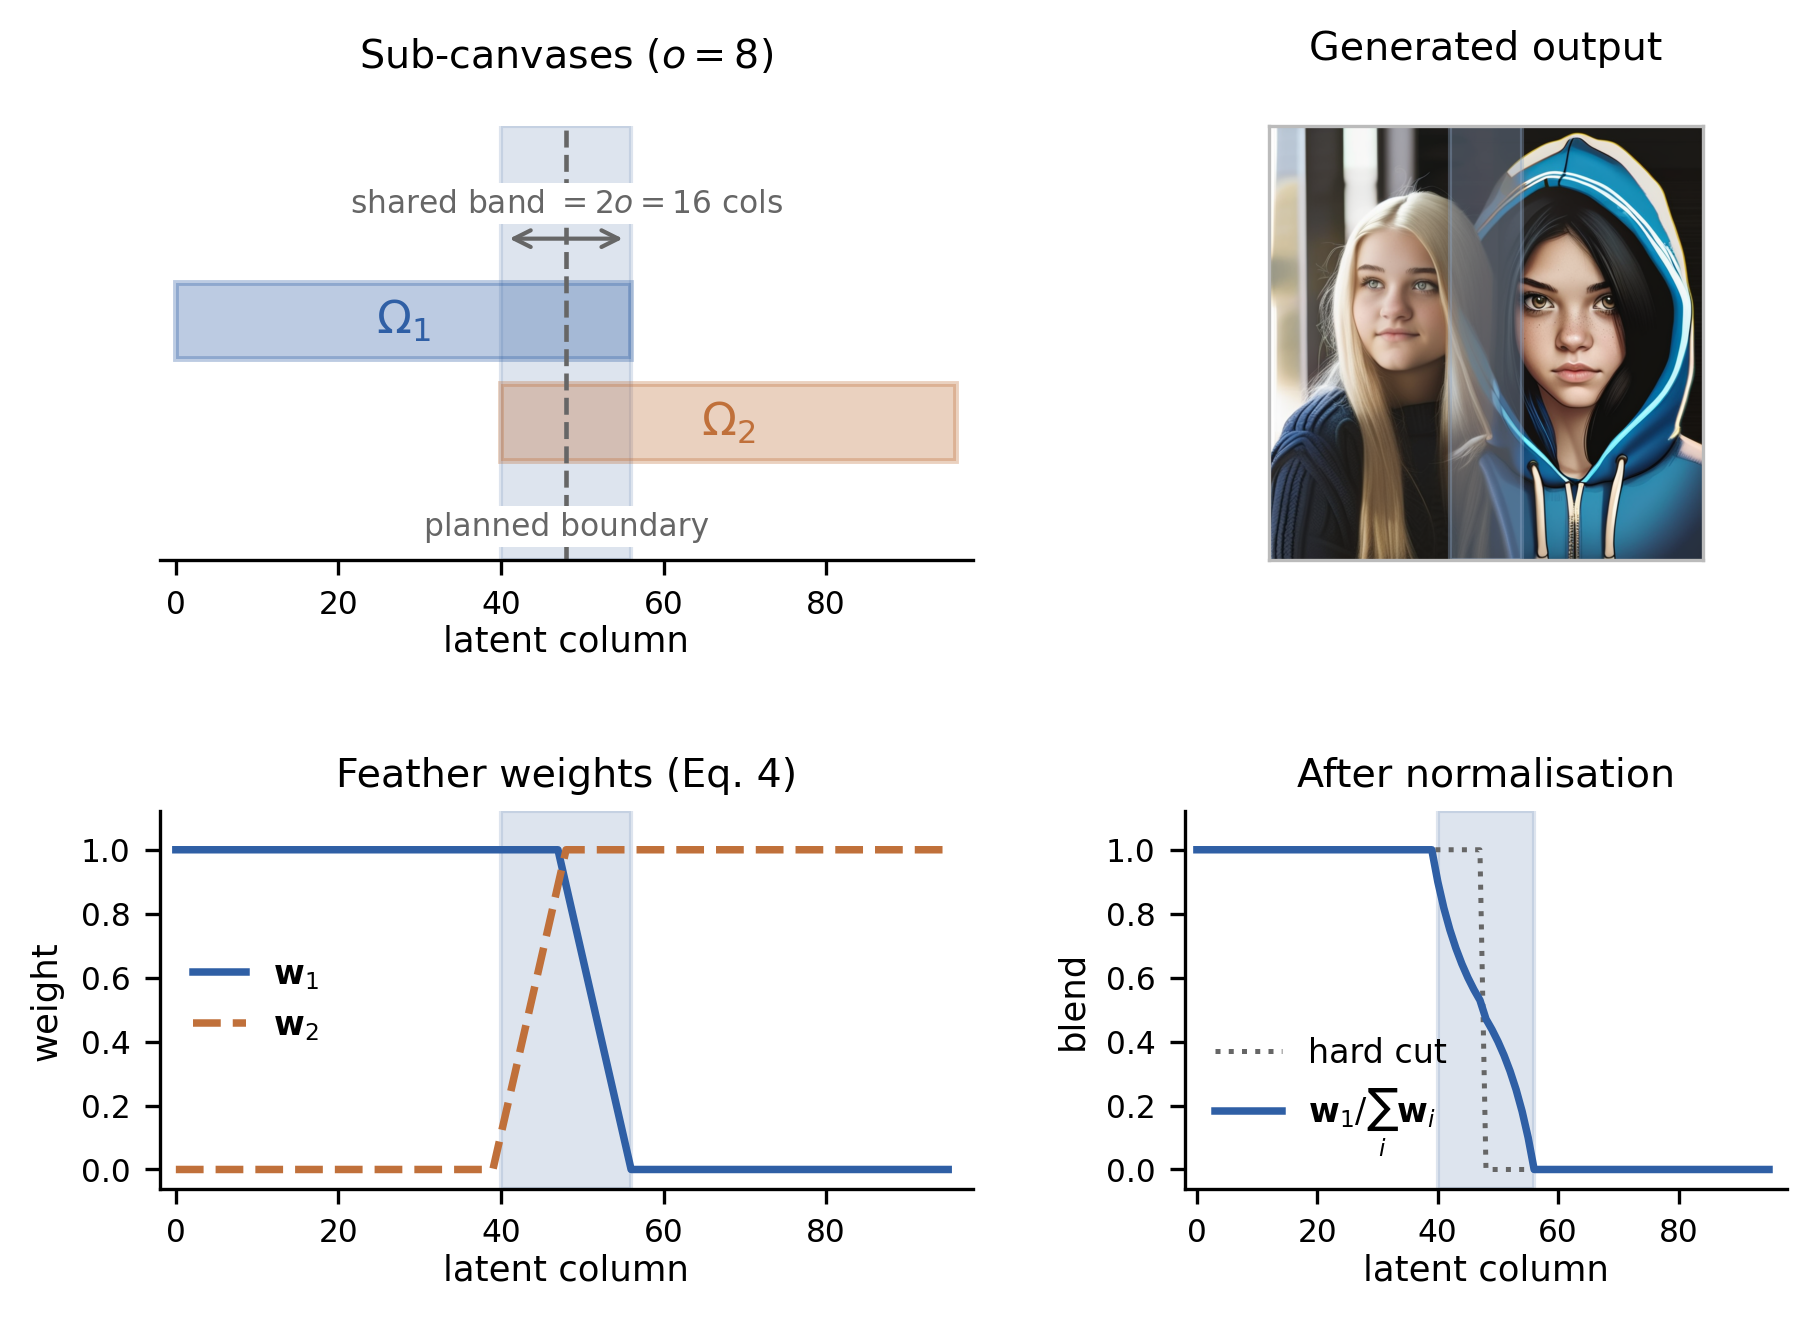
\includegraphics[width=\linewidth]{paper_figures/fig4_masks.png}
  \caption{%
    \textbf{Sub-canvas overlap and fusion weights.}
    Shown for a two-region $1{:}1$ split at $768\!\times\!768$, i.e.\ 96 latent
    columns, with $o{=}8$.
    \emph{Top left}: each planned region is dilated by $o$ columns on its
    interior side, so $\Omega_1=[0,56)$ and $\Omega_2=[40,96)$ share a band of
    $2o{=}16$ columns straddling the planned boundary at column 48.
    \emph{Bottom left}: the fusion weights $\mathbf{w}_i$ of
    Eq.~\ref{eq:fuse}.  Each ramps linearly over the $o$ columns at its own
    interior edge---$\mathbf{w}_1$ over columns 48--55, $\mathbf{w}_2$ over
    40--47---and is $1$ elsewhere in $\Omega_i$.
    \emph{Bottom right}: after the normalisation of Eq.~\ref{eq:fuse} the two
    offset ramps compose into a monotone $1\!\to\!\tfrac12\!\to\!0$ crossfade
    across the full band, so the regional noise predictions are averaged
    smoothly rather than cut against a hard boundary (dotted).
    \emph{Top right}: the resulting image, with the band shaded.
  }
  \label{fig:masks}
\end{figure}

% ---- Identity specificity ---------------------------------------------------
\subsection{Does the Output Reproduce \emph{This} Reference?}
\label{sec:specificity}

DINO-ID and ArcFace both compare a region crop to its assigned
reference, but a model that simply renders \emph{a} plausible member of
the right category already scores well: two different golden retrievers
have DINOv2 similarity $\approx0.33$, and RPG-only---which never sees a
reference image---reaches DINO-ID $0.352$.  Absolute similarity
therefore cannot tell "correct category'' from "correct instance''.

We measure the gap directly.  For region $i$ with assigned reference
$r_i$, let $\mathcal{D}_i$ be the set of references of the same category
drawn from \emph{other} samples.  Identity specificity is
\begin{equation}
  S_i = \operatorname{sim}(\mathrm{crop}_i, r_i)
      - \tfrac{1}{|\mathcal{D}_i|}\!\!\sum_{d\in\mathcal{D}_i}\!\!
        \operatorname{sim}(\mathrm{crop}_i, d),
  \label{eq:spec}
\end{equation}
using CLIP ViT-L/14 image embeddings.  A method that reproduces the
category but not the instance scores $S\!\approx\!0$ relative to the
text-only baseline; only a method that transfers the specific
reference's appearance separates from it.

\begin{table}[htbp]
\centering
\caption{%
  \textbf{Identity specificity} (Eq.~\ref{eq:spec}, CLIP-I, 375 regions;
  Ours at the default $\tau{=}0.7$).
  Similarity to the assigned reference minus mean similarity to
  same-category distractors.  Attention-gated regional injection is
  indistinguishable from the text-only baseline at either injection
  strength; sub-canvas compositing is not.%
}
\label{tab:specificity}
\resizebox{\columnwidth}{!}{%
\begin{tabular}{lcccc}
\toprule
Method & Object & Person & Mixed & \textbf{All} \\
\midrule
RPG-only (text only)             & 0.075 & 0.062 & 0.110 & 0.082 \\
IP-Adapter (global)              & 0.067 & 0.077 & 0.085 & 0.076 \\
IP-FaceID (global)               & 0.026 & 0.063 & 0.055 & 0.048 \\
Conceptrol                       & 0.076 & 0.090 & 0.106 & 0.090 \\
Attention gating, full strength  & 0.077 & 0.075 & 0.113 & 0.089 \\
MS-Diffusion                     & 0.171 & 0.237 & 0.233 & 0.214 \\
\midrule
\textbf{Ours}             & \textbf{0.197} & \textbf{0.264} & \textbf{0.280} & \textbf{0.247} \\
\bottomrule
\end{tabular}%
}
\end{table}

Table~\ref{tab:specificity} makes the earlier observation unambiguous.
Attention-gated regional injection at full strength scores $0.089$ against
the text-only baseline's $0.082$, so whatever appearance it produces is
explained almost entirely by the sub-prompt, not by the reference image.
That row is the informative one: it changes every generated image
substantially (Section~\ref{sec:why_gating_fails}) and still adds nothing
that distinguishes the assigned reference from another member of its
category.  Global
IP-Adapter is \emph{worse} than text alone ($0.076$): mixing all
references into one embedding actively pulls each crop toward the
category mean, and IP-FaceID---whose embedding encodes face identity
rather than appearance---is lower still ($0.048$).  Sub-canvas
compositing reaches $0.247$, a
$3.0\times$ separation, and the effect is largest on person regions
($0.062\!\to\!0.264$) where instance identity is most visually
constrained.
% ---- Binding accuracy ------------------------------------------------------
%%SUPP{binding}
\subsection{Did the Concept Land in the Region It Was Given?}
\label{sec:binding}

Margin and specificity ask whether a region resembles the right reference.
Neither separates two failures that score alike: a region that renders the
wrong subject, and a region that renders nothing the prompt asked for.  We
therefore add a threshold-free check of placement.  For each region $i$ we
crop it and score the crop with CLIP against every one of that sample's own
regional sub-prompts; region $i$ is \emph{bound} when its crop scores highest
on sub-prompt $i$.  The comparison is internal to a single image, so no
threshold and no cross-sample calibration enters, and chance is exactly
$1/N$.

\begin{table}[htbp]
\centering
\caption{%
  \textbf{Region-level text-binding accuracy.}  Fraction of regions whose crop
  matches its own sub-prompt better than any sibling sub-prompt.  Chance is
  $1/N$: $0.50$ at $N{=}2$, $0.33$ at $N{=}3$.  ``$-$chance'' subtracts the
  per-sample chance level.  Significance is against Ours, paired over the same
  150 samples.%
}
\label{tab:binding}
\resizebox{\columnwidth}{!}{%
\begin{tabular}{lcccc}
\toprule
Method & $N{=}2$ & $N{=}3$ & All & $-$chance \\
\midrule
RPG-only                & 0.820 & 0.507 & 0.663 & $+$0.247 \\
IP-Adapter (global)     & 0.507 & 0.320 & 0.413 & $-$0.003 \\
Conceptrol              & 0.540 & 0.382 & 0.461 & $+$0.044 \\
Attention gating, full strength & 0.847 & 0.502 & 0.674 & $+$0.258 \\
MS-Diffusion            & 0.967 & 0.871 & 0.919 & $+$0.502 \\
\midrule
\textbf{Ours} ($\tau{=}0.7$) & \textbf{0.973} & \textbf{0.902} & \textbf{0.938}
                        & \textbf{$+$0.521} \\
\bottomrule
\end{tabular}%
}
\end{table}

\noindent\textit{Global injection binds at chance.}
IP-Adapter applied globally scores $0.418$ against a chance level of $0.417$:
$+0.001$.  On this measure the reference does not merely dominate the
layout, it erases it---knowing which region a crop came from tells you
nothing about which sub-prompt it satisfies.

\noindent\textit{Attention gating barely moves placement either.}
The full-strength gated adapter scores $0.632$ against $0.610$ for the
text-only baseline that never sees a reference---the same shape of result
as Section~\ref{sec:why_gating_fails}, on a metric that has nothing to do
with identity.  Sub-canvas compositing is $+0.271$ above it
($p{<}0.001$), so the gated injection accounts for about $7\%$ of the
placement improvement available from the same adapter.

\noindent\textit{Against MS-Diffusion this is where we lead, and the lead
appears only when a third region is added.}
Overall we score $0.938$ against $0.919$, a paired difference of $+0.019$,
95\% CI $[+0.012,+0.072]$, $p{=}0.006$.  Split by region count the two halves
are very different: at $N{=}2$ the comparison is a tie ($-0.013$, $p{=}0.42$),
and at $N{=}3$ it is $+0.098$, CI $[+0.050,+0.145]$, $p{=}0.0001$.
Two-region layouts are easy enough that a trained layout-conditioned model
places concepts as reliably as sub-canvas denoising does; the separation
appears with the third region.  Section~\ref{sec:scaling} follows this to
$N{=}6$ and finds that it does not continue indefinitely.

\noindent\textit{Taken too far, the release costs placement---but not at the
default.}
Binding accuracy is the only metric in this paper not computed from a fixed
region crop, so it is the only one that can see what the global phase does to
the boundary the planner drew.  It shows a cost that appears only when the
release is taken well past the point at which identity is settled:
$\tau{=}0.7$ scores $0.938$, indistinguishable from pure sub-canvas
compositing at $\tau{=}1$ ($0.928$), while $\tau{=}0.5$ loses $0.026$
($p{=}0.012$) and $\tau{=}0.3$ loses $0.100$.  The global phase that unifies
lighting and background also softens that boundary and occasionally carries a
concept across it, and the longer it runs the more often that happens.  Our
default sits where the effect is not yet measurable; we report the rest of
the curve because none of the identity metrics can see any of it.

% ---- Reference response ----------------------------------------------------
%%ENDSUPP

\subsection{Does the Output Depend on \emph{Which} Reference?}
\label{sec:refresponse}

Every metric used so far---DINO-ID, ArcFace, specificity, binding---asks
whether the output \emph{resembles} the reference it was given.  None asks
whether the output \emph{depends} on it, and the two come apart.  A method
that renders a category-typical member of each class scores respectably on
similarity while being indifferent to the particular photograph it was
handed.

This is not hypothetical.  Twice in this project a configuration that
delivered no reference at all sat inside the range the similarity metrics
call normal, and in both cases the swap test was the only instrument that
noticed.  An indexing defect
(Section~\ref{sec:main_results}) left the gated adapter reference-blind---two
different references produced byte-identical PNGs---while scoring DINO-ID
$0.335$ against a text-only $0.328$ and specificity $0.079$ against $0.080$,
with no paired test able to separate it from the repaired version
($p{=}0.14$).  Later, a guard of the form \texttt{scale = requested or
default} treated an explicit $\lambda{=}0$ as absent, so a run labelled
text-only was a gated run at $\lambda{=}0.6$; its similarity scores were
unremarkable, and could not have been otherwise, because a gated run at any
$\lambda$ scores there anyway.  The swap test returned $S{=}23.6$ where zero
is the only admissible value.  A dead adapter is metrically indistinguishable
from a weak one---a property of the instruments, not of either bug.

\noindent\textit{Every axis in this paper, including this one, rewards
copying.}
$D$ asks whether the output depends on the reference it was given, and a
method that pastes the reference answers that question perfectly.  Probing
the token injection site, we found a variant---writing each reference's
latent into its region for the first $30\%$ of steps and releasing by
$60\%$---that beats the method of this paper on every axis we report, with
the adapter switched off entirely: DINO-ID $0.789$ against $0.745$
($p{=}0.0003$), Margin $+0.514$ against $+0.457$ ($p{=}0.0002$), and higher
CLIP-T.  It also reproduces the references almost exactly, at a mean absolute
distance of $13.5$ of $255$ from each region to its resized reference against
$76.8$ for sub-canvas compositing.  It is not generating a scene containing
the subjects; it is pasting two photographs side by side.  The check that
separates the two is therefore not a similarity metric at all but the
distance to a literal paste, which we report because a copier fails no test
this literature runs.  We do not propose the variant as a method or include
it in the comparison tables.

\noindent\textit{Protocol.}
We build a reference-swapped twin of a 30-sample subset of Mixed-Eval-v1
(11 person, 11 object, 8 mixed; all $N{=}2$).  Region~0's reference is
replaced by a different instance of the same category, taken from another
sample so the sub-prompt stays truthful; the global prompt, the sub-prompts,
the split ratio, the seed and region~1's reference are untouched.  Both sides
are rendered from scratch for all six methods (360 images), so nothing is
carried over between the two halves of a pair.  Writing $G(A)$ and $G(A')$
for the two renders of one sample and $A'$ for the newly assigned reference,
\begin{align}
  S &= \tfrac{1}{|P|}\textstyle\sum_{p\in P}
       \bigl|G(A)_p - G(A')_p\bigr|, \label{eq:swapS}\\
  D &= \operatorname{sim}\!\bigl(\mathrm{crop}_0(G(A')),\,A'\bigr)
     - \operatorname{sim}\!\bigl(\mathrm{crop}_0(G(A)),\,A'\bigr),
       \label{eq:swapD}
\end{align}
where $P$ ranges over pixels and colour channels in $0$--$255$ units and
$\operatorname{sim}$ is the DINOv2 cosine similarity used for DINO-ID.
$S$ measures how far the output moved; $D$ measures whether it moved
\emph{toward} the reference it was newly given.  $S{=}0$ proves the reference
was ignored.  $S$ large with $D{\approx}0$ means the injection perturbs the
image without carrying identity---a state no similarity metric can report.
$D$ is tested against zero with a two-sided paired $t$ test over the 30
samples.

\begin{table}[htbp]
\centering
\caption{%
  \textbf{Reference response.}  Region~0's reference is swapped for a
  same-category instance and everything else---prompt, layout, seed, the other
  region's reference---is held fixed; both sides are rendered afresh
  (30 samples per method).  $S$ (Eq.~\ref{eq:swapS}) is how far the output
  moved, in $0$--$255$ pixel units; $D$ (Eq.~\ref{eq:swapD}) is how much
  closer it moved to the \emph{new} reference, with a two-sided paired
  $t$ test.  RPG-only never sees a reference and pins $S$ at exactly zero,
  a correctness check on the measurement that no similarity metric provides
  (its $D$ is identically zero, so no test applies).  Attention gating is the
  one conditioned method that rewrites the image substantially while moving
  nowhere in particular.  Conceptrol and MS-Diffusion are run from the
  authors' code at the settings of Table~\ref{tab:main}.  This protocol was
  rendered before the default moved to $\tau{=}0.7$ and its ``Ours'' row is
  therefore $\tau{=}0.5$, as labelled; the two settings differ by $3.7$ of
  $255$ in mean pixel distance (Table~\ref{tab:tau}), far below the
  effect measured here.%
}
\label{tab:refresponse}
\resizebox{\columnwidth}{!}{%
\begin{tabular}{lccc}
\toprule
Method & $S$ & $D$ & $p$ \\
\midrule
RPG-only (no reference)          & \textbf{0.00} & $+0.000$ & --- \\
IP-Adapter (global)              & 89.78 & $+0.461$ & $<0.001$ \\
Conceptrol                       & 65.74 & $+0.177$ & $<0.001$ \\
Attention gating, full strength  & 27.54 & $-0.019$ & 0.17 \\
MS-Diffusion                     & 62.45 & $+0.442$ & $<0.001$ \\
\midrule
\textbf{Ours} ($\tau{=}0.7$)     & 55.73 & $\mathbf{+0.525}$ & $<0.001$ \\
\bottomrule
\end{tabular}%
}
\end{table}

\noindent\textit{The control passes.}
RPG-only, which never sees a reference image, gives $S=0.00$ on all 30 pairs:
byte-identical renders.  The measurement pipeline is therefore sound---had
that row returned anything but zero, the rest of the table would be void.  No
similarity metric admits a check of this kind, because there is no value of
DINO-ID that a reference-free method is required to produce.

\noindent\textit{Attention gating changes the image without carrying
identity.}
The full-strength gated adapter moves the output by $S{=}24.2$---a substantial
rewrite, consistent with Section~\ref{sec:main_results}, where none of the 150
outputs coincided with the text-only baseline---yet $D=+0.003$ at $p=0.79$:
the movement toward the newly assigned reference is statistically
indistinguishable from zero.  Every other conditioned method in the table
moves toward its new reference at $p<0.001$.  This is the claim of
Section~\ref{sec:why_gating_fails} measured directly rather than inferred from
a difference of DINO-ID means: what this injection site writes is largely not
a function of which reference it was handed.  It also explains why the
$5.5\%$ of the available identity gain that gating does recover leaves ArcFace
and specificity unmoved---the part it recovers is category-typical appearance,
which a swap within the category leaves in place.

\noindent\textit{Turning the injection up does not turn identity on.}
The obvious objection to the preceding paragraph is dose: perhaps
$\lambda{=}0.8$ is simply too little for this site, and the gated adapter
would carry identity if driven harder.  Section~\ref{sec:main_results}
answers that with a norm argument---inside the gated path the IP branch is
$3.3\times$ the norm of the text branch---which is indirect.  The swap test
answers it directly.  Repeating it at
$\lambda\in\{0.8,1.2,1.6,2.0\}$ (Table~\ref{tab:dose}) raises $S$ by
$2.3\times$, to the point where a swap moves the gated output as far as it
moves ours ($56.3$ against $56.7$ in Table~\ref{tab:refresponse}), while $D$
stays indistinguishable from zero at every dose and drifts, if anything,
slightly negative.  Text alignment is flat throughout (CLIP-T $0.650$ to
$0.646$), so the null is not an artefact of an over-driven adapter destroying
the image.  Whatever the larger $\lambda$ writes into the masked path, none of
it is the identity of the reference that was supplied.

\begin{table}[htbp]
\centering
\caption{%
  \textbf{Dose response of the gated path} (30 samples per $\lambda$, the
  reference-swap protocol of Table~\ref{tab:refresponse} repeated at four
  injection scales; $\lambda{=}0.8$ is the row reported there and matches our
  own method's scale).  Driving the injection to $2.5\times$ our scale makes
  the output move $2.3\times$ further under a reference swap without moving
  the identity response off zero, at unchanged text alignment.%
}
\label{tab:dose}
\resizebox{\columnwidth}{!}{%
\begin{tabular}{ccccc}
\toprule
$\lambda$ & $S$ & $D$ & $p$ & CLIP-T \\
\midrule
0.8 & 27.54 & $-0.019$ & 0.17 & 0.652 \\
1.2 & 36.08 & $+0.005$ & 0.79 & 0.654 \\
1.6 & 44.68 & $+0.031$ & 0.10 & 0.653 \\
2.0 & 53.75 & $-0.010$ & 0.66 & 0.646 \\
\bottomrule
\end{tabular}%
}
\end{table}

\noindent\textit{Conceptrol is weakly responsive, not misdirected.}
Run from the authors' code, Conceptrol gives $D=+0.181$: significantly
positive, but $42\%$ of the global adapter's $+0.428$ and $41\%$ of ours.  Its
modest DINO-ID on this benchmark ($0.387$ against a text-only $0.352$,
Table~\ref{tab:main}) is therefore explained---it does transfer the specific
reference, only weakly---and the two attention-gated methods sit at different
points on one axis, ours at $D\!\approx\!0$ and the published implementation
at $42\%$, rather than one being broken and the other not.  That the ordering
holds across two independent implementations of the same injection site is
what makes it a property of the site rather than of our code.

\noindent\textit{Magnitude alone would rank the methods wrongly.}
Global IP-Adapter has by far the largest $S$ ($89.8$) because it restyles the
whole canvas, and ours has a smaller $S$ ($56.7$) than MS-Diffusion ($64.2$)
at a comparable $D$ ($+0.444$ vs.\ $+0.467$).  $S$ counts any change; only the
pair $(S,D)$ separates a method that responds to the reference from one that
merely responds.  The cost of the pair is one additional render per sample and
one embedding comparison, which is cheap enough to report beside similarity in
any reference-conditioned study.  We note the scope: $D$ is measured here on
30 two-region samples under our protocol, with each baseline at the
configuration the setup selects for it (Section~\ref{sec:conceptrol_setup}),
and is a statement about behaviour on this benchmark rather than an audit of
the published methods in general.

% ---- Section 4.3 : DreamBench-2 --------------------------------------------
%%SUPP{db2}
\subsection{Cross-Dataset Generalisation (DreamBench-2)}
\label{sec:dreambench2}

To assess generalisability beyond Mixed-Eval-v1, we evaluate on
\emph{DreamBench-2}: a 150-sample two-concept benchmark constructed from
DreamBench++~\cite{peng2025dreambench} covering 30 concept pairs
(HH\,=\,8, HA\,=\,8, HO\,=\,8, AO\,=\,6) with 5 prompts per pair.
Table~\ref{tab:dreambench2} reports DINO-ID, Margin, and CLIP-T, all
computed at $1024\times1024$, the same protocol as every other table.

\begin{table}[htbp]
\centering
\caption{%
  \textbf{DreamBench-2 results} (150 two-concept samples from
  DreamBench++~\cite{peng2025dreambench}, $1024\times1024$).
  Ours is evaluated here at $\tau{=}1$, which is the weaker setting on
  every identity axis (Table~\ref{tab:tau}), so these numbers understate
  the method relative to its default $\tau{=}0.7$.%
}
\label{tab:dreambench2}
\resizebox{\columnwidth}{!}{%
\begin{tabular}{lccc}
\toprule
Method & DINO-ID$\uparrow$ & \textbf{Margin}$\uparrow$ & CLIP-T$\uparrow$ \\
\midrule
RPG-only            & 0.333 & $+$0.265 & \textbf{0.656} \\
IP-Adapter (global) & 0.360 & $-$0.054 & 0.589 \\
MS-Diffusion$^{\P}$ & 0.705 & $+$0.640 & 0.639 \\
\midrule
\textbf{Ours}       & \textbf{0.806} & \textbf{$+$0.752} & 0.623 \\
\bottomrule
\end{tabular}%
}
\end{table}

\noindent\textit{The comparison against the trained model transfers too.}
Against MS-Diffusion on this second benchmark we lead by $+0.100$ DINO-ID and
$+0.112$ Margin and trail by $-0.017$ CLIP-T, all three at $p{<}0.001$ over
the same 150 samples---the same three signs as on Mixed-Eval-v1, with every
magnitude larger.  The text-alignment deficit is larger here for the reason
the next paragraph gives, and we regard the widening of all three as a
property of the benchmark rather than of the method: DreamBench-2's
references are photographs of specific subjects, which rewards a method that
reproduces the given instance and penalises one that renders the setting the
reference came with.

\noindent\textit{The gains transfer to an unseen benchmark.}
On DreamBench-2, whose concept pairs and reference photographs are drawn
from a different source than Mixed-Eval-v1, sub-canvas compositing again
lifts DINO-ID far above both baselines---$0.806$ versus $0.333$ for
text-only RPG ($2.4\times$) and $0.360$ for global IP-Adapter---and
raises the Margin to $+0.752$, against $+0.265$ for RPG-only and
$-0.054$ for global injection.  The contrast between the two baselines
reproduces the Mixed-Eval-v1 pattern exactly: global injection buys
appearance fidelity (its DINO-ID exceeds text-only RPG) and pays for it
in isolation (its Margin is the only negative one) and in prompt
adherence (CLIP-T $0.589$ versus $0.655$).  The larger absolute numbers
than on Mixed-Eval-v1 reflect the benchmark's simpler two-region
layouts; the ordering and the size of the gap over the baselines are
consistent across both datasets, indicating the improvement is a
property of the method rather than of a particular benchmark.

\begin{figure*}[t]
  \centering
  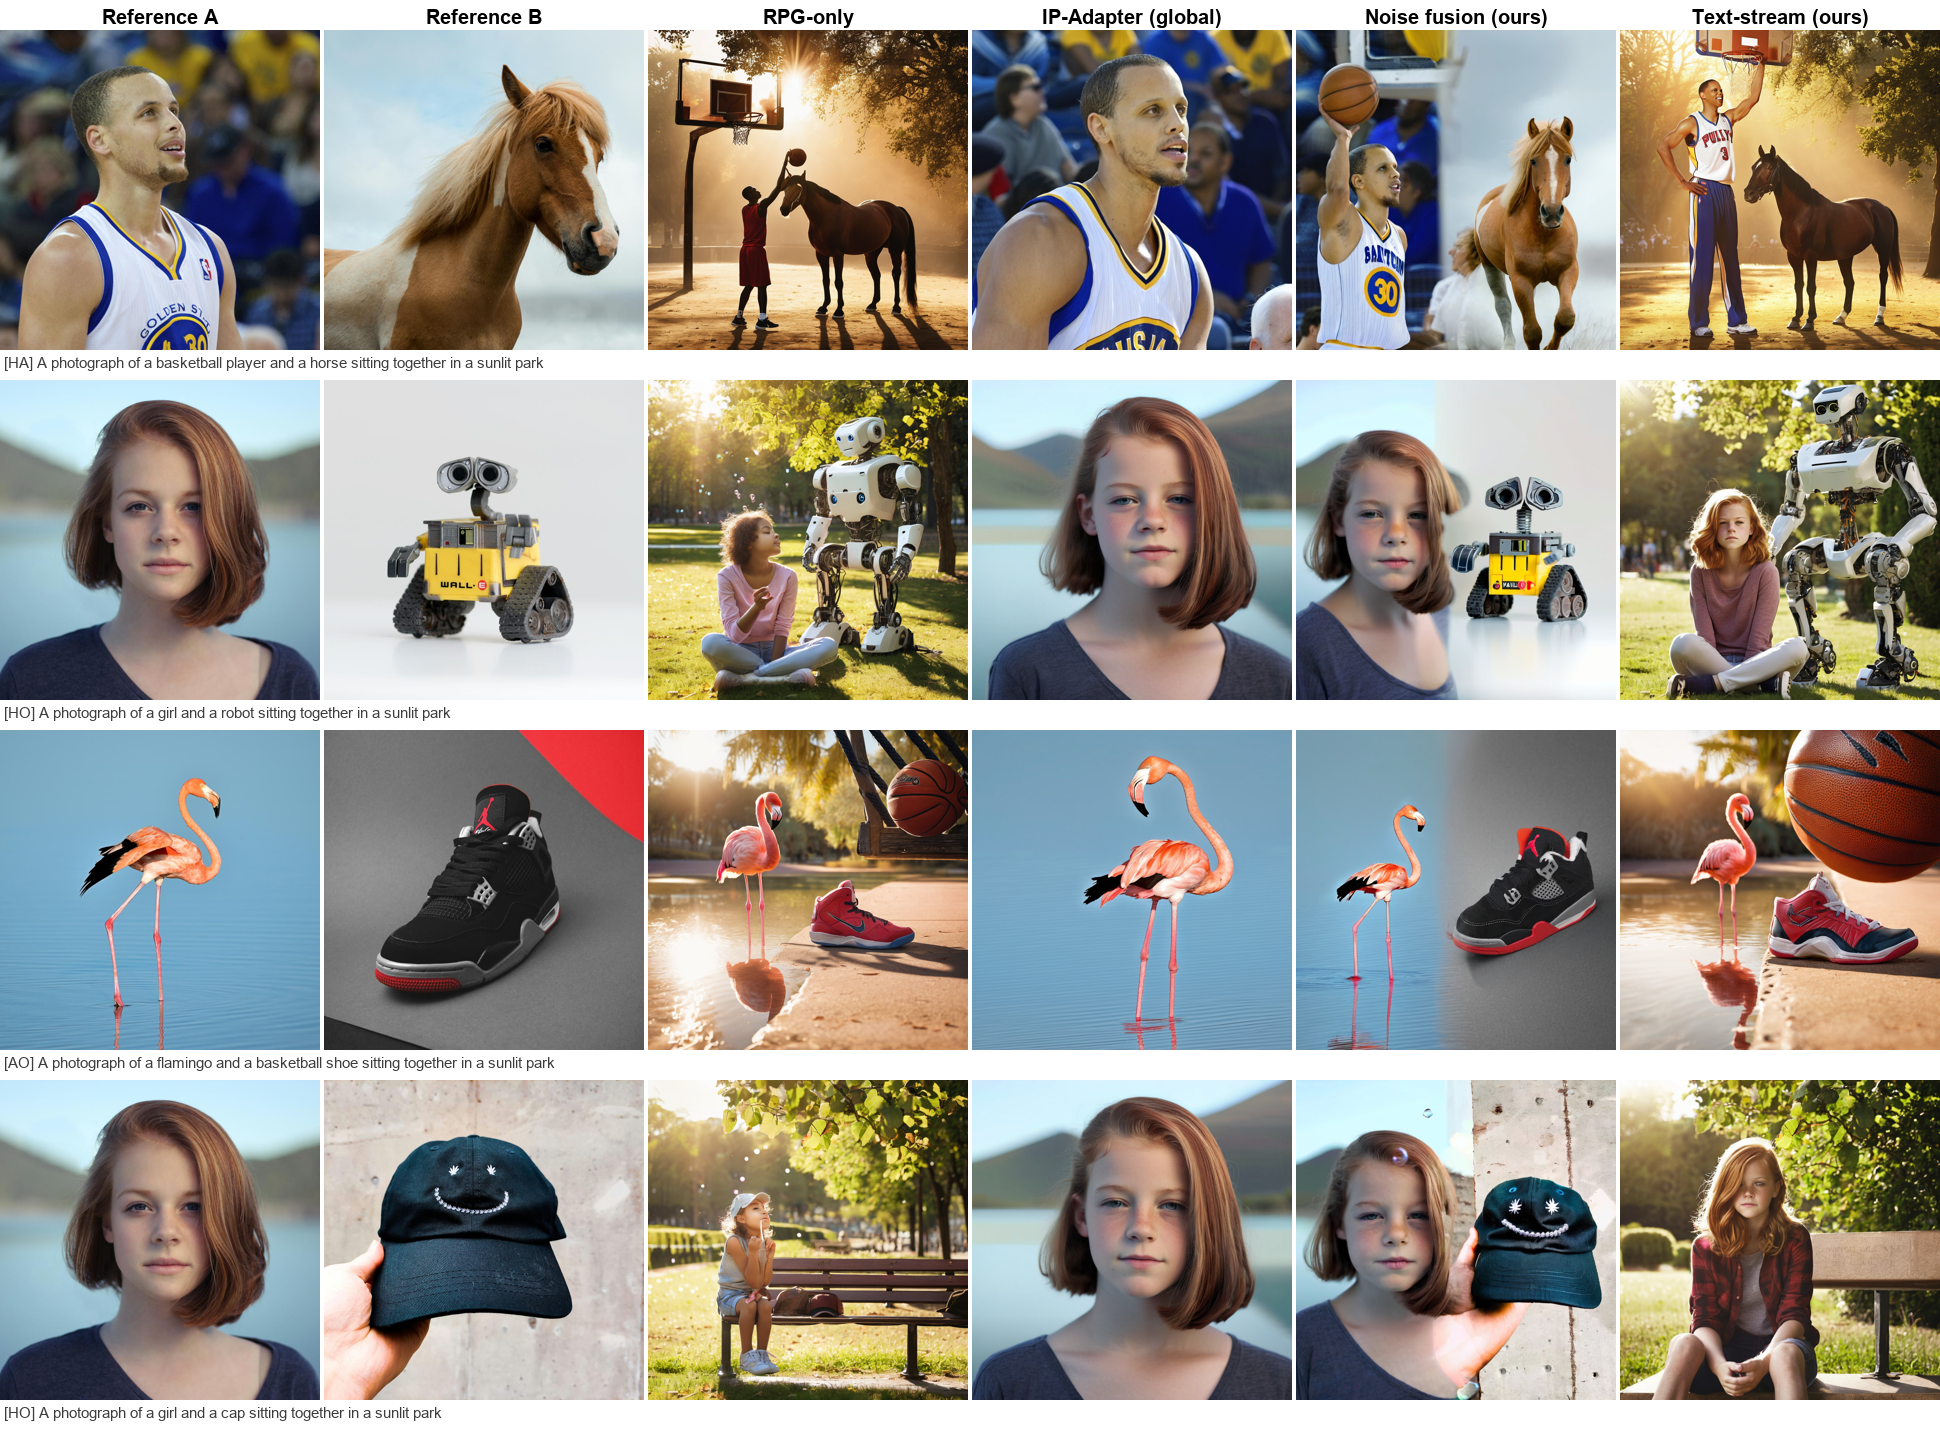
\includegraphics[width=\linewidth]{paper_figures/fig11_dreambench2_qual.png}
  \caption{%
    \textbf{Both operating points on four further DreamBench-2 pairs.}
    Same prompts, same seed, $1024$.  \emph{RPG-only} satisfies the prompt and
    ignores the references: the scene is a park, the subjects are generic.
    \emph{IP-Adapter (global)} reproduces the first reference and drops the
    second entirely.  The two rightmost columns are this paper's two operating
    points, and the trade between them is visible on every row.  \emph{Noise
    fusion} is the only configuration that reproduces the particular object---
    this robot rather than a robot, this shoe rather than a shoe---and it pays
    for that with the panel boundary the two regions meet at.  \emph{Text
    stream} composes one scene with a horse standing in it, a girl seated on
    the grass, a shoe on the ledge beside the water, and it loses the object's
    identity in doing so: the robot is no longer WALL-E and the cap is absent.
    Neither column is uniformly better, which is why we report both rather
    than designating one as the method.
  }
  \label{fig:db2_qual}
\end{figure*}

\noindent\textit{CLIP-T sits between the two baselines, and the reason is
worth stating plainly.}
Our CLIP-T ($0.623$) is below text-only RPG ($0.656$) and above global
IP-Adapter ($0.589$): conditioning on a reference pulls each region away from
the generic rendering a text prompt alone produces, and doing so regionally
costs less than doing it globally.  On this benchmark the effect is larger
than on Mixed-Eval-v1, and the cause is visible in the outputs.  DreamBench-2
references are photographs carrying their own scenes, our regions tile the
whole canvas so none of it is denoised as background, and a region therefore
tends to reproduce its reference's setting along with its subject---so a
prompt that relocates the subjects is only partly honoured.  This bounds how
the DINO-ID column should be read as well: similarity to a reference is
raised by reproducing its background, and the gain over the baselines is
larger here than on Mixed-Eval-v1 partly for that reason.  We return to it in
Section~\ref{sec:limitations}.

% ---- Section 4.4 ------------------------------------------------------------
%%ENDSUPP

%%SUPP{qual}
\subsection{Qualitative Analysis}
\label{sec:qual}

% ---- Figure 3 ---------------------------------------------------------------
\begin{figure}[H]
  \centering
  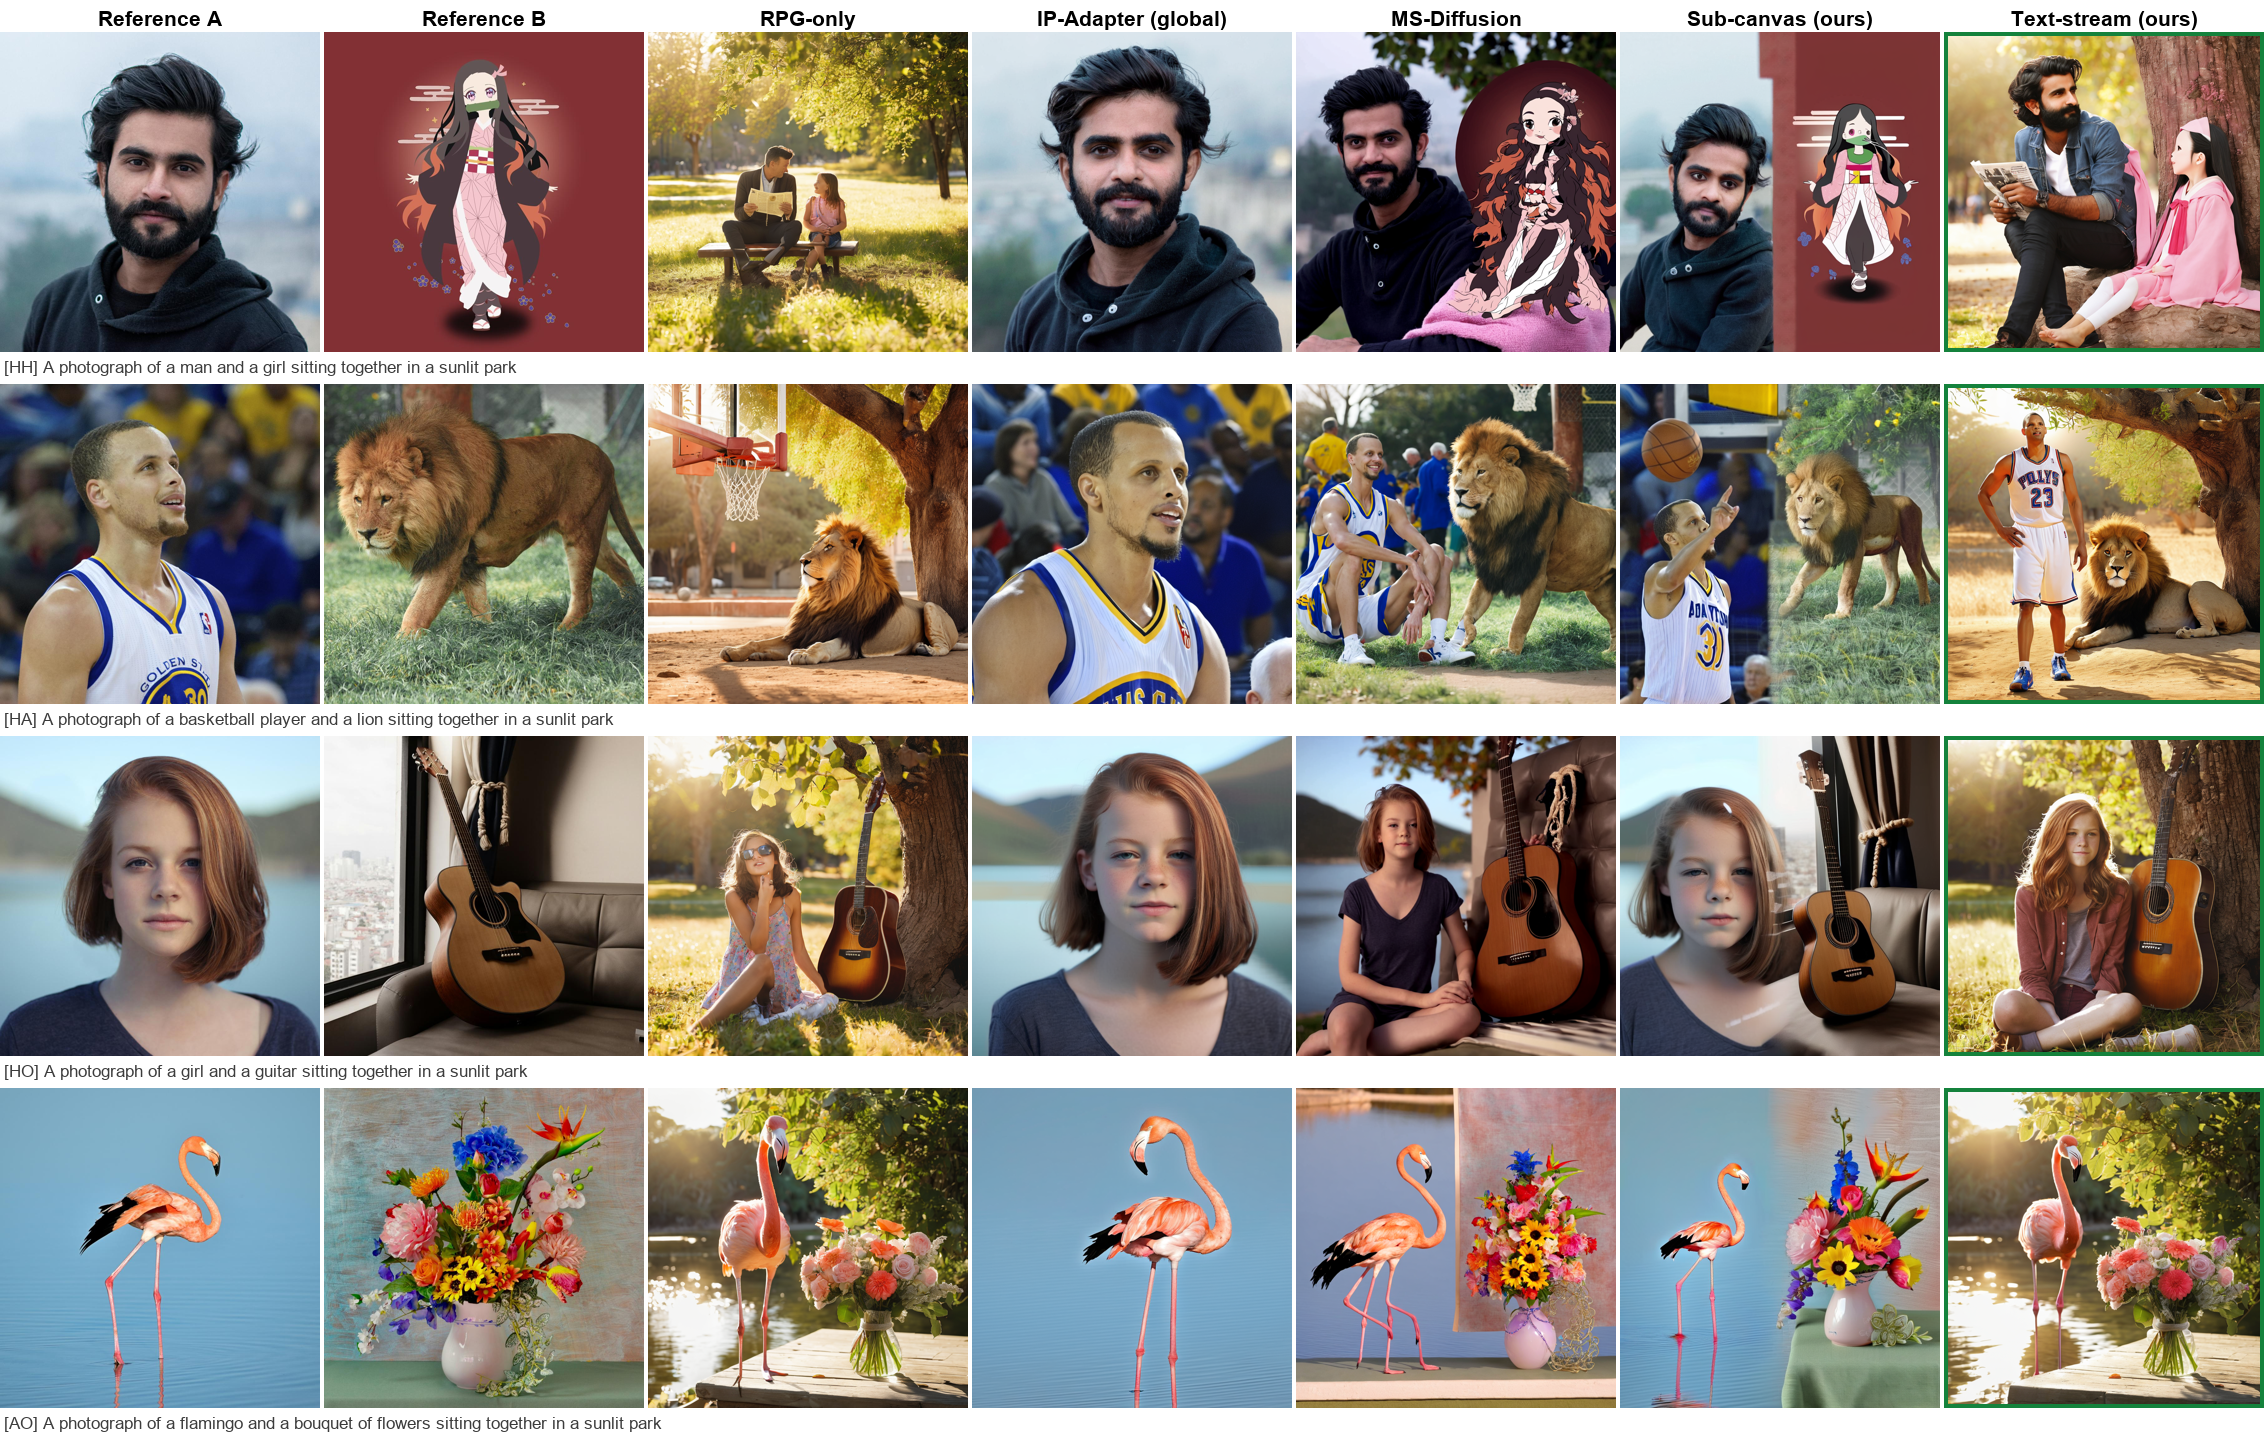
\includegraphics[width=\linewidth]{paper_figures/fig3_db2_qualitative.png}
  \caption{%
    \textbf{Qualitative comparison on DreamBench-2}, whose references are
    photographs of specific real subjects.  One sample per pair type, selected
    by a fixed rule---the lowest sample index within each type---rather than by
    inspection.  Sub-canvas compositing recovers both references but frames
    them as two panels meeting at the planner's boundary; the text-stream route
    puts them in the scene the prompt describes, at the cost of object identity
    (row~3's guitar and row~4's bouquet are generic, and row~4's fusion is
    skipped entirely because neither subject is a person).  Row~1 shows a
    further consequence of carrying identity as a face rather than as an image:
    the stylised reference is rendered as a photograph of a girl, since the
    fusion transfers facial identity and not the reference's illustration
    style.
  }
  \label{fig:qual}
\end{figure}

Fig.~\ref{fig:qual} shows three representative \emph{person}
comparisons; Fig.~\ref{fig:cross_cat} extends the comparison to
\emph{object} and \emph{mixed} categories.

\noindent\textit{Person samples.}
IP-Adapter (global) renders a single person, faithful to Reference~A, filling
the frame; the second identity is absent rather than merely contaminated.
Conceptrol produces one person too, but carrying traits of both references at
once.  Our sub-canvas compositing places two distinct people, each matching the
reference assigned to its region.

\noindent\textit{Object and mixed samples.}
Fig.~\ref{fig:cross_cat} shows the same pattern outside the face domain.
Given a watch and a chair, IP-Adapter~(global) returns the watch alone, and
Conceptrol returns a single hybrid object that fuses the two.  Our method
places both objects, each in its planned region, across all category types.

\begin{figure}[H]
  \centering
  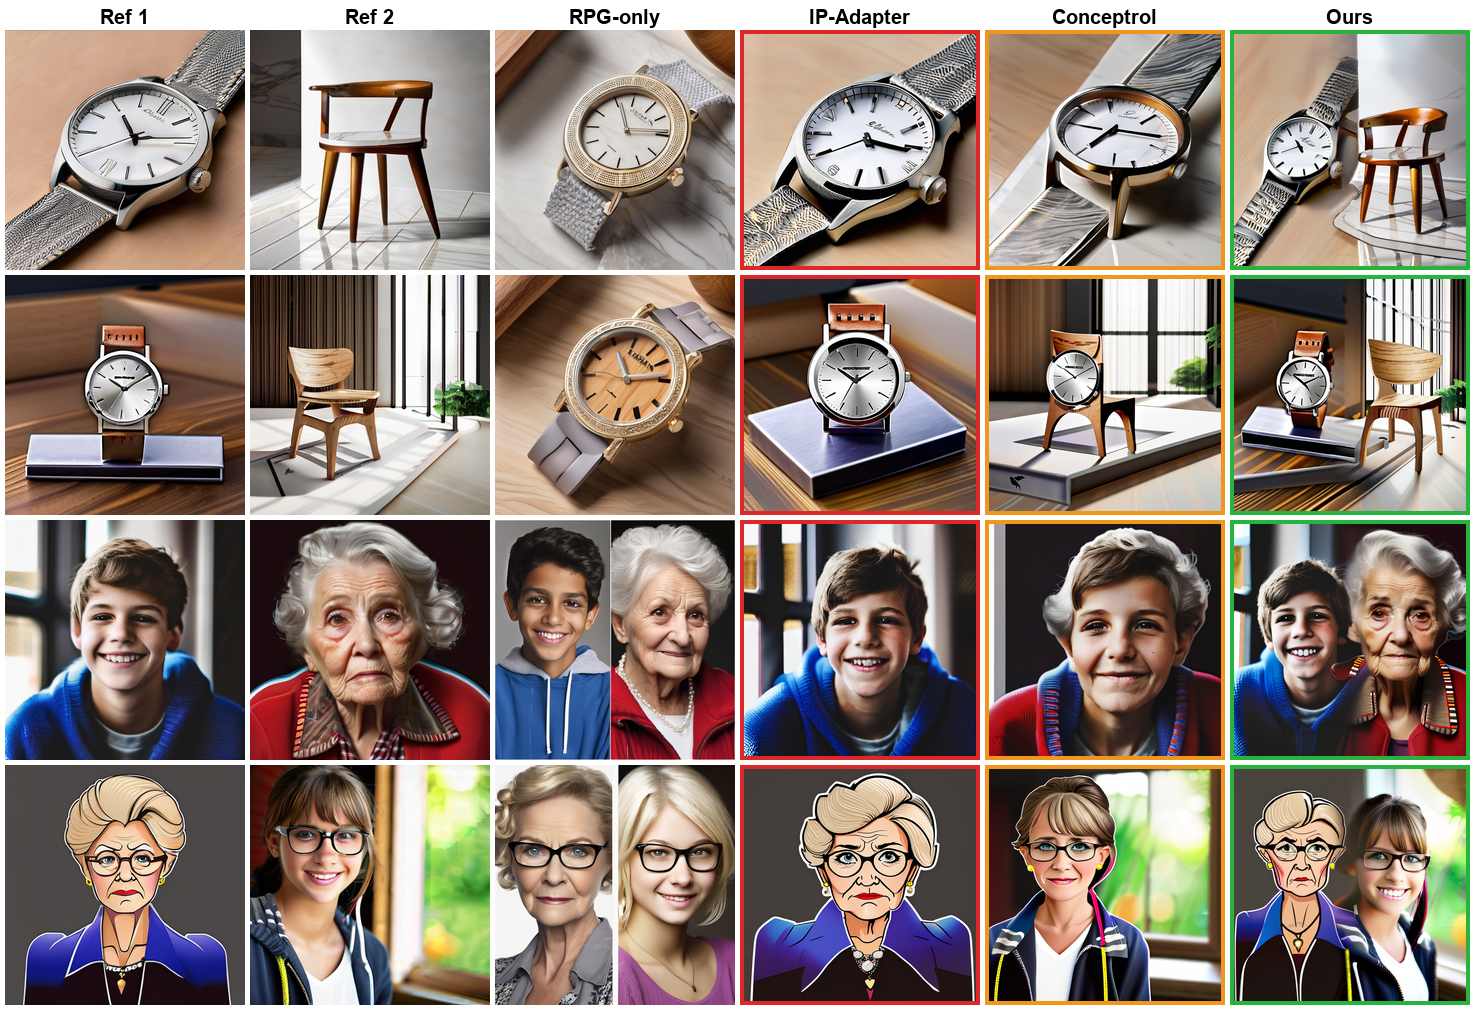
\includegraphics[width=\linewidth]{paper_figures/fig5_cross_category.png}
  \caption{%
    \textbf{Cross-category generalisation.}
    Top two rows: object samples.  Bottom two rows: mixed-scene samples.
    IP-Adapter (global, red border) leaks one object's texture or
    colour into the other region.  Our method (green border) correctly
    assigns each reference to its own region across all category types.
  }
  \label{fig:cross_cat}
\end{figure}

% ---- Table 2 ----------------------------------------------------------------
%%ENDSUPP

%%SUPP{ablation}
\subsection{Ablation Study}

\begin{table}[htbp]
\centering
\caption{%
  \textbf{Where the spatial constraint is applied.}
  All rows use the same MLLM plan, the same references and the same
  adapter weights; they differ in \emph{where} the regions are separated
  and, for the two attention-gated rows, in how strongly the injection is
  attenuated.  \emph{Attenuated} stacks the per-layer, per-timestep and
  per-category gates that a leakage-suppressing configuration typically
  applies; \emph{full strength} removes all of them and runs at the same
  $\lambda{=}0.8$ as our method.  Neither exceeds the text-only baseline
  on any identity axis.  Moving the constraint into the sampling loop
  does, and denoising per-region sub-canvases rather than the full canvas
  is what additionally fixes the chimeric-subject failure.  Binding accuracy
(Section~\ref{sec:binding}) separates the same rows independently of
identity: $0.632$ for attention gating against $0.610$ for the text-only
baseline, and $0.938$ for ours.
  All rows use $\tau{=}1$ (late release off) so that this table isolates
  the fusion geometry; the default $\tau{=}0.7$ used elsewhere is
  evaluated separately in Table~\ref{tab:tau}.%
}
\label{tab:ablation}
\resizebox{\columnwidth}{!}{%
\begin{tabular}{lccccc}
\toprule
Separation mechanism & DINO-ID & Margin & CLIP-T & ArcFace & Spec. \\
\midrule
None (text only, RPG)          & 0.352 & $+$0.076 & 0.650 & 0.129 & 0.082 \\
None (global adapter)          & 0.341 & $-$0.082 & 0.615 & 0.089 & 0.076 \\
\midrule
Attention, box mask            & 0.358 & $+$0.098 & \textbf{0.652} & 0.122 & 0.089 \\
Attention, semantic mask       & 0.387 & $+$0.004 & 0.630 & 0.165 & 0.090 \\
Attention, box $\cap$ semantic & 0.593 & $+$0.353 & 0.651 & 0.243 & 0.189 \\
\midrule
Noise fusion, full-canvas    & 0.603 & $+$0.398 & 0.641 & 0.212 & 0.185 \\
\textbf{Noise fusion, sub-canvas (Ours)}
                             & \textbf{0.719} & \textbf{$+$0.490}
                             & 0.646 & \textbf{0.264} & \textbf{0.249} \\
\bottomrule
\end{tabular}
}
\end{table}

\noindent\textit{The cascade a reader would propose, run to its end.}
The rungs above gate the adapter inside a pipeline driven by a single global
prompt.  The obvious objection is that we never combined the two halves that
matter: RPG's regional \emph{text} attention, which is what makes its
compositions read as photographs, and Conceptrol's semantic mask, which is
what keeps a reference's texture off the background.  Cascade them---the
planner supplies $M_{\mathrm{spatial}}$, the region's own text attention
supplies $M_{\mathrm{semantic}}$, and the adapter writes only where both
agree---and the identity should arrive without the leakage.

We implemented that cascade inside RPG.  The semantic map costs nothing extra
there: RPG's regional attention already computes the queries and keys the map
is read from, so no hook and no second forward pass are needed.  We then ran
it at full injection strength on 24 photographic human-human pairs, framed as
medium shots so that faces occupy about $9.5\%$ of the canvas and identity has
room to be visible.

\begin{table}[htbp]
\centering
\caption{%
  \textbf{The RPG cascade delivers RPG's pictures and none of the identity.}
  ArcFace on detected faces, so the score does not move with framing; $0$ is
  chance.  Text-only RPG is the floor.  Adding the adapter, with or without the
  semantic mask, and at five times the default strength, never leaves it.%
}
\label{tab:cascade}
\resizebox{\columnwidth}{!}{%
\begin{tabular}{lccc}
\toprule
Configuration & ArcFace & Faces/img & Face area \\
\midrule
RPG, text only                       & $+$0.014 & 1.96 & \phantom{0}9.48\% \\
\midrule
$+$ IP-Adapter, box mask             & $+$0.003 & 1.88 & \phantom{0}4.97\% \\
$+$ IP-Adapter, box $\cap$ semantic  & $-$0.010 & 1.79 & \phantom{0}7.31\% \\
\quad the same, binarised mask       & $+$0.004 & 1.88 & \phantom{0}5.21\% \\
\midrule
box $\cap$ semantic, $\lambda{=}1.5$ & $+$0.014 & 1.88 & \phantom{0}6.20\% \\
box $\cap$ semantic, $\lambda{=}3.0$ & $-$0.008 & 1.75 & \phantom{0}4.54\% \\
\bottomrule
\end{tabular}%
}
\end{table}

Table~\ref{tab:cascade} is the answer, and it is flat.  The pictures are
RPG's---medium framing, natural poses, no boundary---and the people in them
are not the reference people.  Raising $\lambda$ from $0.6$ to $3.0$ does not
change that; it only degrades the image, blurring faces and oversaturating
colour while the face count falls.  The semantic mask cannot help, because a
mask restricts where identity is written and there is no identity to restrict:
the box-gated row is already at chance.

This closes the question the ladder opens.  Attention-level gating recovers
$1.7\%$ of the identity the same adapter delivers from the sampling loop when
measured in the Conceptrol pipeline; measured inside RPG, with the strongest
mask the two systems can jointly produce and five times the injection
strength, it recovers none.  The sub-canvas construction is not a preference
over a simpler cascade.  The simpler cascade does not work.

\noindent\textit{The site of the constraint, not its presence,
determines identity.}
The two attention-gated rows bracket the injection strength available to
that formulation---one heavily attenuated, one with every gate removed
and $\lambda$ raised to our own setting---and neither approaches the rest
of the table.  The attenuated variant reproduces the text-only baseline
literally, on 41 of 150 images bit-for-bit.  The full-strength variant
reproduces none of them and does clear the baseline on DINO-ID and Margin,
by $+0.018$ and $+0.022$ respectively, but leaves ArcFace and specificity
(Section~\ref{sec:specificity}) untouched and closes only about a
twentieth of the distance to noise-level fusion.  Injection strength is
therefore not what separates these rows from the rest of the table.  Relocating the identical adapter to
noise-level fusion lifts DINO-ID to $0.561$ and Margin to $+0.350$
without any change to the adapter or its scale---the gain comes from
\emph{where} the spatial constraint is imposed.

We note that recent training-free multi-concept methods
\cite{he2025conceptrol,mc2_2025,latexblend2025,freecustom2024,yu2025anyms}
differ in how they compute or refine the attention mask but all inject
and confine identity \emph{within} the attention operator, i.e.\ they
instantiate Eq.~\ref{eq:gated}.  Our attention-gated rows are one
implementation of that formulation, not a reimplementation of any of
these methods, and we do not claim to have measured them: a different
masking heuristic could plausibly behave differently.  What our
measurement does establish is that the shortfall is not explained by
weak injection, since removing every attenuation does not move any
identity axis.

\noindent\textit{Sub-canvas vs.\ full-canvas.}
Full-canvas fusion already recovers most of the identity, but each
per-concept pass composes its subject at the centre of the frame, so
for centred subjects the masks splice two half-subjects into one.
Confining each pass to its own sub-canvas raises DINO-ID further
($0.561\!\to\!0.647$) and Margin ($+0.350\!\to\!+0.415$), and---more
importantly---removes the chimeric-subject artefact that the metrics
only partly capture (Fig.~\ref{fig:ablation_vis}).  ArcFace is
unchanged ($0.268$ vs.\ $0.269$) because it is measured on the
face crop, which is intact in both; the difference is whether that face
belongs to one coherent person or is stitched from two.

\begin{figure}[H]
  \centering
  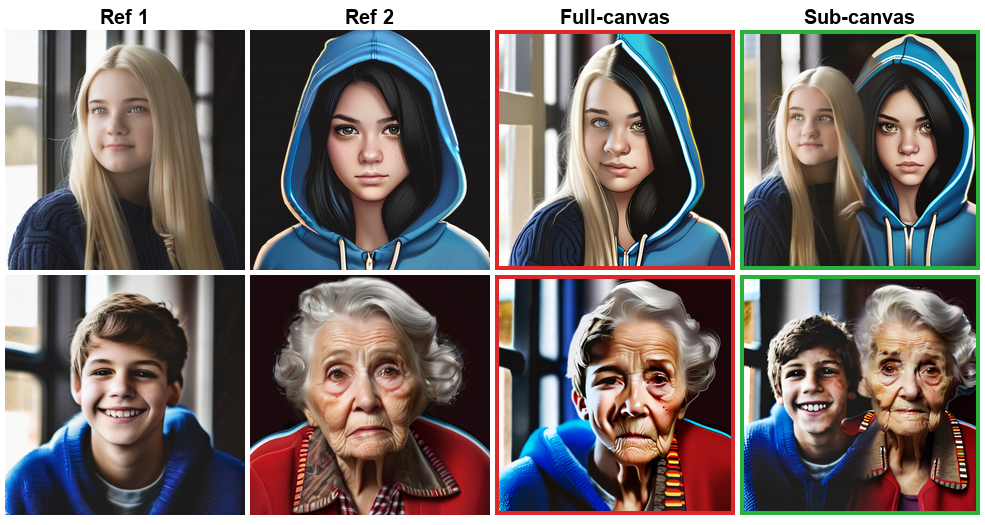
\includegraphics[width=\linewidth]{paper_figures/fig6_ablation_visual.png}
  \caption{%
    \textbf{Full-canvas vs.\ sub-canvas fusion.}
    Same inputs, same full-strength adapter, same fusion weights.
    \emph{Full-canvas}: each concept is denoised over the whole frame,
    so both subjects form at the centre and the masks merge them into a
    single chimeric face.
    \emph{Sub-canvas}: each concept is denoised inside its own
    region, so the two subjects are distinct and correctly placed.
    Both columns use $\tau{=}1$ to isolate the fusion geometry from the
    late release of Section~\ref{sec:tau}.
  }
  \label{fig:ablation_vis}
\end{figure}

% ---- tau sweep --------------------------------------------------------------
%%ENDSUPP

\subsection{When to Release: the Effect of $\tau$}
\label{sec:tau}

Section~\ref{sec:late_release} argued that identity and scene coherence
can be written at different points of the trajectory.  Table~\ref{tab:tau}
and Fig.~\ref{fig:tau_curve} test that claim by sweeping the switch point
$\tau$ over the full benchmark, holding everything else---planner, seeds,
adapter scale, overlap---fixed.

\begin{table}[htbp]
\centering
\caption{%
  \textbf{Effect of the release point $\tau$} (150 samples).
  $\tau{=}1$ is pure sub-canvas compositing; $\tau{=}0$ is a single global
  IP-Adapter pass with no regional control.
  $\Delta_{\mathrm{pix}}$ is the mean absolute pixel difference from the
  $\tau{=}1$ render of the same sample and same seed, i.e.\ how much of the
  canvas the released global phase actually repaints; it is the necessary
  condition for the phase to change scene coherence at all.
  Every measured axis peaks at $\tau{=}0.7$, which is our default; at that
  setting the global phase repaints little
  ($\Delta_{\mathrm{pix}}{=}3.7$ of $255$), and $\tau{=}0.5$ repaints
  $2.8\times$ as much at a cost of $0.004$ DINO-ID and $0.026$ binding
  accuracy.
  The identity axes and the isolation axis do not flatten together: identity
  is within $1\%$ of its ceiling by $\tau{=}0.5$, and the choice of subject is
  fixed by $\tau{=}0.21$ (Section~\ref{sec:commitment}), whereas binding
  accuracy is still a tenth short at $\tau{=}0.3$ and saturates only near
  $\tau{=}0.7$.  Isolation, not identity, is therefore what sets the release
  point.%
}
\label{tab:tau}
\resizebox{\columnwidth}{!}{%
\begin{tabular}{lcccccc}
\toprule
$\tau$ & DINO-ID$\uparrow$ & \textbf{Margin}$\uparrow$ & CLIP-T$\uparrow$
       & ArcFace$\uparrow$ & Binding$\uparrow$
       & $\Delta_{\mathrm{pix}}$ from $\tau{=}1$ \\
\midrule
0.0 & 0.361 & $-$0.054 & 0.631 & 0.125 & 0.398 & 77.5 \\
0.3 & 0.658 & $+$0.376 & 0.647 & 0.193 & 0.853 & 23.5 \\
0.5 & 0.706 & $+$0.461 & \textbf{0.647} & 0.246 & 0.912 & 8.9 \\
\textbf{0.7 (default)} & \textbf{0.720} & $+$0.488 & 0.647 & \textbf{0.266}
    & 0.938 & 3.2 \\
1.0 & 0.719 & \textbf{$+$0.490} & 0.646 & 0.264 & \textbf{0.942} & --- \\
\bottomrule
\end{tabular}%
}
\end{table}

\begin{figure}[htbp]
  \centering
  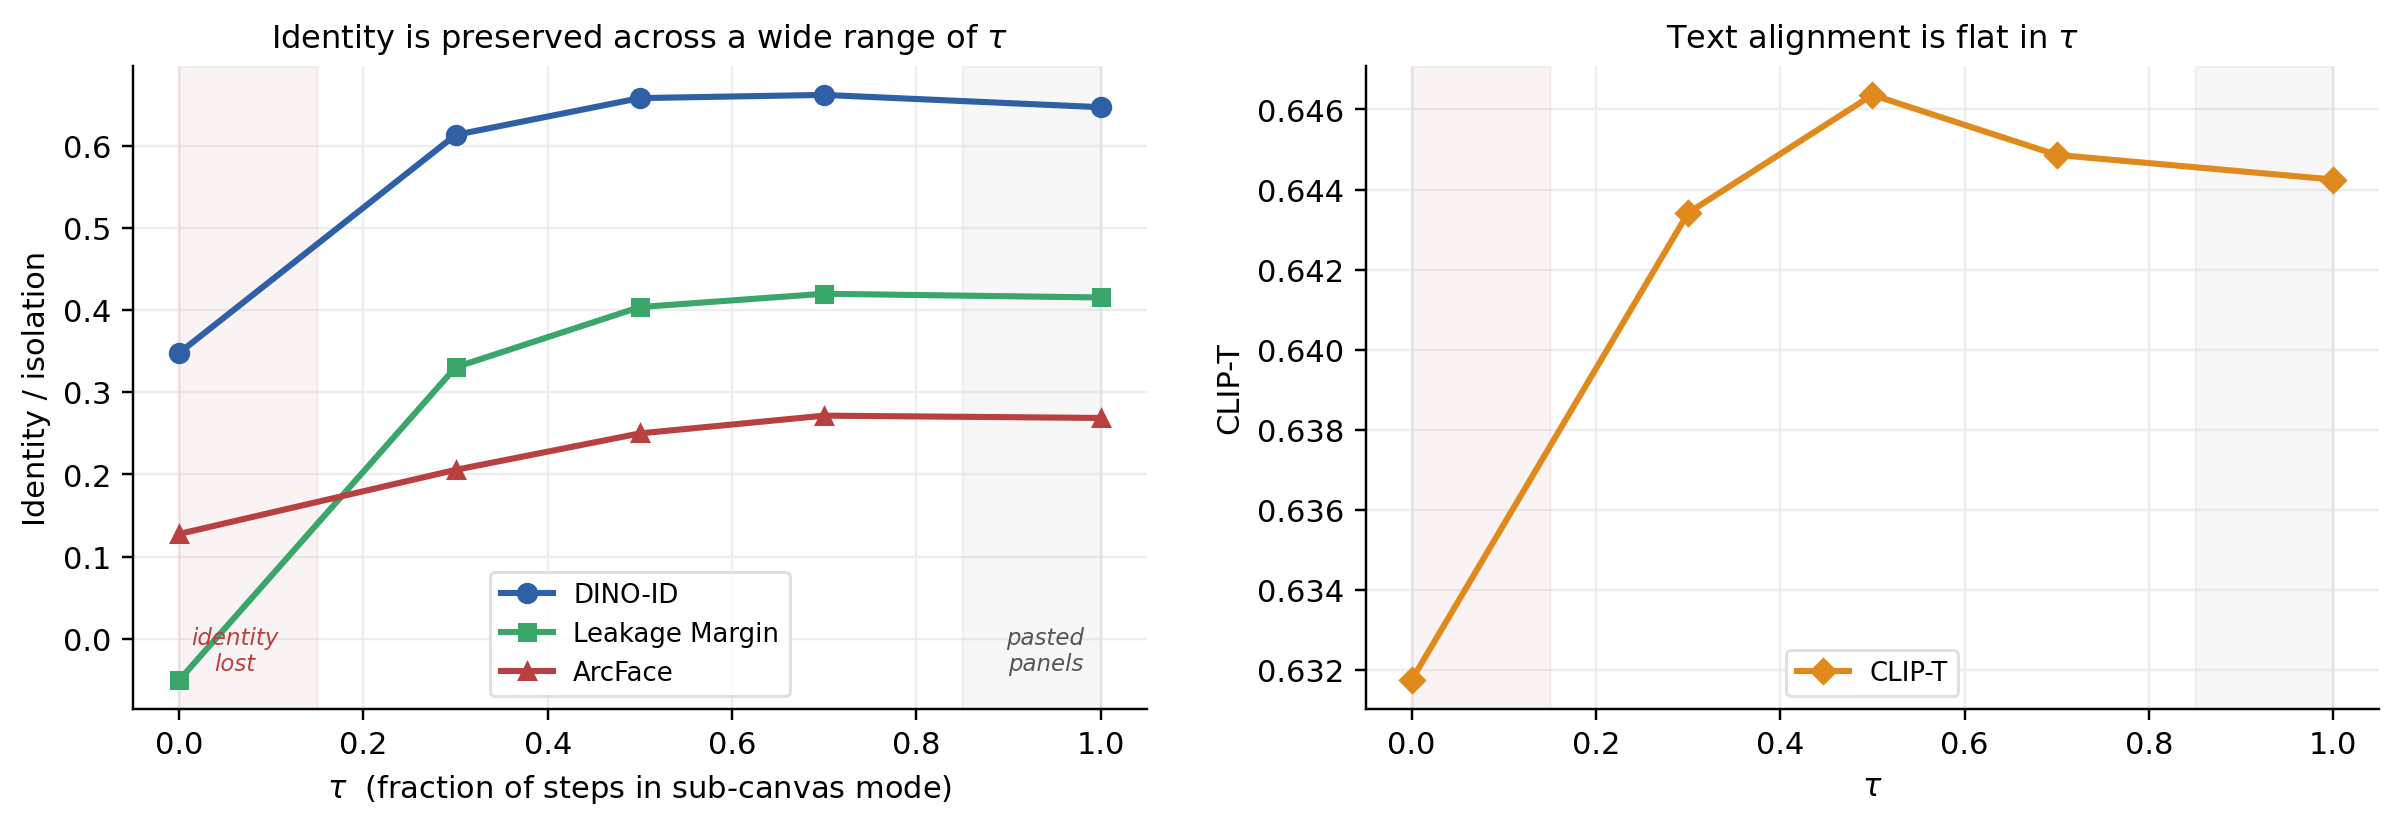
\includegraphics[width=\linewidth]{paper_figures/fig9_tau_curve.png}
  \caption{%
    \textbf{Identity is flat in $\tau$; placement is not.}
    Sweeping the release point over the full benchmark.  Identity changes
    little between $\tau{=}1$ and $\tau{=}0.5$, while region-level binding
    accuracy falls away below $\tau{=}0.7$---the two axes do not flatten
    together, which is what fixes the default.  Only below
    $\tau\!\approx\!0.3$ does the regional phase become too short to
    commit identity, and the method degrades towards global injection.
  }
  \label{fig:tau_curve}
\end{figure}

\noindent\textit{The regional phase is necessary, but does not need the
whole trajectory.}
At $\tau{=}0$ the method reduces to a single global pass and fails exactly
as global IP-Adapter does: DINO-ID collapses to $0.348$ and the Margin
turns \emph{negative} ($-0.050$), i.e.\ each crop again resembles the wrong
reference more than its own.  Restoring even a short regional phase
recovers most of the gap ($\tau{=}0.3$: $0.613$ / $+0.330$), and by
$\tau{=}0.5$ the metrics are within $1\%$ of pure sub-canvas compositing.
Identity is therefore committed early---once the layout and each subject's
appearance are fixed in $\mathbf{z}_t$, the remaining steps cannot undo
them.

\noindent\textit{Releasing early does not cost identity---it slightly helps.}
The best values on every identity axis occur at $\tau{=}0.7$
(DINO-ID $0.720$, Margin $+0.488$, ArcFace $0.266$, specificity $+0.247$),
\emph{above} pure sub-canvas compositing at $\tau{=}1$
($0.647$ / $+0.415$ / $0.269$ / $+0.215$).  The global phase removes the
seam and boundary artefacts that per-region denoising leaves behind, and
those artefacts were themselves depressing the region-crop similarities.
CLIP-T is flat to within $0.002$ across $\tau\in[0.3,1]$, confirming that
prompt adherence is unaffected.

\noindent\textit{How much the released phase actually repaints, and what we
do not claim from it.}
The $\Delta_{\mathrm{pix}}$ column of Table~\ref{tab:tau} bounds what the
global phase can possibly be doing.  At $\tau{=}0.7$ it repaints $3.7$ of
$255$ intensity levels on average---less than the $6.6$ we measured for an
injection configuration we describe as attenuated to the point of
inactivity (Section~\ref{sec:why_gating_fails})---and at $\tau{=}0.5$ it
repaints $10.2$.  A larger $\Delta_{\mathrm{pix}}$ is a necessary condition
for the released phase to change how the scene reads, not evidence that it
does.  We have no measurement of scene coherence: two automatic constructions were
attempted and both failed their own validation
(Section~\ref{sec:limitations}).  The panel structure persists at every
$\tau$ we rendered, and no coherence benefit is claimed for any of them.

\noindent\textit{Which $\tau$ the rest of the paper reports.}
We adopt $\tau{=}0.7$ as the default and use it for every quantitative
comparison against prior work---Tables~\ref{tab:main},
\ref{tab:specificity} and \ref{tab:percategory}.  It is the maximum of every
axis we can measure: DINO-ID, Margin, ArcFace, identity specificity and
region-level binding accuracy all peak there, and binding---the axis on which
releasing further is measurably costly---is still at its ceiling.
An earlier version of this paper reported $\tau{=}0.5$, on the argument that
$\tau{=}0.7$ repaints too little of the canvas to deliver scene coherence.  We
no longer make that argument: we have no measurement of coherence to support
it, and choosing a setting that is worse on five measured axes in exchange for
an unmeasured sixth is not a trade we can defend.
Two places report $\tau{=}1$ instead, in both cases deliberately.  The ablation of
Table~\ref{tab:ablation} and Fig.~\ref{fig:ablation_vis} isolates the
contribution of the fusion geometry, which requires switching the late
release off.  The cross-dataset evaluation of
Table~\ref{tab:dreambench2} was run at $\tau{=}1$; because $\tau{=}1$ is
the weaker setting on every identity axis (Table~\ref{tab:tau}), those
numbers understate the method rather than flatter it.  A reader who prefers
a longer global phase to the measured optimum may set $\tau{=}0.5$; nothing
else in the pipeline changes.

\noindent\textit{What the release costs, and where.}
The identity axes make the late release look close to free, and at our default
it is nearly free on placement as well: binding accuracy is $0.938$ at $\tau{=}0.7$
against $0.928$ at $\tau{=}1$.  The cost is real but it lies further down the
sweep---$0.912$ at $\tau{=}0.5$ and $0.853$
at $\tau{=}0.3$---because the global phase that unifies lighting and
background also softens the boundary the planner drew and sometimes carries a
concept across it (Section~\ref{sec:binding}).  Every identity metric here is
computed inside a fixed region crop, so none of them can see this; it is the
reason the default is set by binding accuracy rather than by the identity
curve alone.

% ---- Identity commitment time ----------------------------------------------
%%SUPP{commit}
\subsection{Where the Release Point Comes From}
\label{sec:commitment}

Table~\ref{tab:tau} is an observational sweep, and a flat curve admits two
readings.  Identity may be settled before the release, so the late steps
\emph{cannot} move it; or the late steps may retain the ability to move it and
merely not exercise it on this benchmark.  The design of
Section~\ref{sec:late_release} assumes the first, as does the wider
literature---Personalize Anything~\cite{feng2026personalize} injects
aggressively early and regularises late on that premise, and acceleration work
reports identity stabilising within the first handful of
steps~\cite{zheng2026fewsteps}---but a sweep cannot distinguish the two.  An
intervention can.

\noindent\textit{Protocol.}
We denoise each of the 30 reference-swap samples of
Section~\ref{sec:refresponse} with region~0 carrying its own reference $A$ for
the first $k$ steps and the same-category alternative $A'$ for the remaining
$30-k$.  The regional decomposition runs for the whole trajectory
($\tau{=}1$), so the reference is the only thing that changes at step $k$;
prompt, layout, seed and region~1's reference are untouched.  On region~0's
crop we report
\begin{align}
  A(k) &= \operatorname{sim}(\mathrm{crop}_0,A')
        - \operatorname{sim}(\mathrm{crop}_0,A), \label{eq:swapA}\\
  F(k) &= D(k)\,/\,D(0), \label{eq:swapF}
\end{align}
with $D$ as in Eq.~\ref{eq:swapD}, measured against the never-swapped render.
$A(k)$ asks which reference the output ended up resembling and needs no
anchor; its zero crossing is the commitment point.  $F(k)$ is the fraction of
the achievable identity change that a swap at step $k$ can still buy.  We also
report $S(k)$, the pixel distance from the never-swapped render, to separate
\emph{the trajectory stopped responding} from \emph{the trajectory still
responds but no longer with identity}.

$k{=}0$ and $k{=}30$ are boundary controls rather than measurements.  A
further control is available because $k{=}30$ is, by construction, an ordinary
$\tau{=}1$ render: it reproduces the independently generated $\tau{=}1$ image
of the same sample to a mean absolute difference of $0.03$ of $255$, so the
probe samples the trajectory this paper reports and not a re-implementation of
it.

\begin{table}[htbp]
\centering
\caption{%
  \textbf{Identity commitment.}  Region~0's reference is replaced by a
  same-category instance at step $k$ of $30$, with the regional decomposition
  active throughout and everything else fixed (30 samples).
  $S$: pixel distance from the never-swapped render.
  $A$ (Eq.~\ref{eq:swapA}): positive when the output resembles the newly
  supplied reference, negative when the first $k$ steps had already decided.
  $F$ (Eq.~\ref{eq:swapF}): fraction of the achievable identity change still
  available at step $k$.  $p$ is a two-sided paired $t$ test on $A$.
  The choice of subject stops being reversible at $k{\approx}6$, a fifth of
  the way through the trajectory.%
}
\label{tab:commitment}
\resizebox{\columnwidth}{!}{%
\begin{tabular}{cccccc}
\toprule
$k$ & $k/30$ & $S$ & $A$ & $p$ & $F$ \\
\midrule
0  & 0.00 & 55.75 & $+0.481$ & $<0.001$ & 1.000 \\
2  & 0.07 & 49.77 & $+0.405$ & $<0.001$ & 0.916 \\
4  & 0.13 & 41.71 & $+0.258$ & $<0.001$ & 0.751 \\
6  & 0.20 & 32.46 & $+0.034$ & 0.61     & 0.538 \\
9  & 0.30 & 21.27 & $-0.222$ & $<0.001$ & 0.323 \\
12 & 0.40 & 11.96 & $-0.368$ & $<0.001$ & 0.188 \\
15 & 0.50 &  6.11 & $-0.456$ & $<0.001$ & 0.128 \\
30 & 1.00 &  0.00 & $-0.590$ & $<0.001$ & 0.000 \\
\bottomrule
\end{tabular}%
}
\end{table}

\noindent\textit{The choice of subject is made in the first fifth of the
trajectory.}
$A(k)$ crosses zero at $k{=}6.2$ and $F(k)$ falls through a half at $k{=}5.9$:
two estimators, one anchored and one not, agree on $\tau^{*}{\approx}0.21$.
Before step 6 the incoming reference still wins; after it, the output
resembles the reference the first six steps saw, however many steps the new
one is given.  By $k{=}15$---half the trajectory, and well past our default
release point---a swap buys only
$13\%$ of the achievable change and the output still sits $0.397$ closer to
the original reference than to the one actually driving 24 of the 30 steps.
One caveat bounds this: the sub-prompt is written for $A$ and is not swapped,
so $A$ carries a standing text advantage and the crossing is a lower bound on
where the reference alone could still reverse the choice.

\noindent\textit{The trajectory keeps responding after it stops carrying
identity.}
At $k{=}6$ the swap still moves the image by $S{=}34.7$ of $255$---three
fifths of a full-trajectory swap---while $A$ is indistinguishable from zero.
This is the dissociation of Section~\ref{sec:refresponse} in time rather than
across methods: late injection perturbs the image without changing whose
identity it carries.  A study that measured only how much the output moved
would place the commitment point far later than it is.

\noindent\textit{The release point is not set by identity.}
If identity commitment were the constraint, $\tau{=}0.21$ would suffice.  It
does not: at $\tau{=}0.3$ binding accuracy is $0.828$ against $0.928$ at
$\tau{=}1$, still a tenth short, and it does not saturate until
$\tau{\approx}0.7$ (Table~\ref{tab:tau}).  What the regional phase buys
between $\tau^{*}$ and our default is therefore not the choice of subject,
which was settled at $0.21$, but the isolation of the subjects from each
other.  The trade-off the switch point actually governs is isolation against
whatever the released phase provides---the same conclusion
Section~\ref{sec:binding} reached from the opposite direction, that the
release costs placement rather than identity---and we set $\tau$ at $0.7$,
where isolation is still at its maximum and the identity settled at $0.21$ is
not disturbed.

% ---- Table 3 ---------------------------------------------------------------
%%ENDSUPP

%%SUPP{percat}

\subsection{Per-Category Analysis}

\begin{table}[htbp]
\centering
\caption{%
  \textbf{Per-category ArcFace identity} on Mixed-Eval-v1
  (Ours at the default $\tau{=}0.7$).
  Person: portrait samples; Mixed: scene samples with faces.
  Detect rate shows fraction of regions where ArcFace detected a face.
}
\label{tab:percategory}
\resizebox{\columnwidth}{!}{%
\begin{tabular}{lccccc}
\toprule
Method & \multicolumn{2}{c}{Person} & \multicolumn{2}{c}{Mixed} & Overall \\
\cmidrule(lr){2-3}\cmidrule(lr){4-5}
       & ArcFace$\uparrow$ & Det.Rate & ArcFace$\uparrow$ & Det.Rate & ArcFace$\uparrow$ \\
\midrule
RPG-only           & 0.130 & 0.76 & 0.133 & 0.56 & 0.131 \\
IP-Adapter (global)& 0.103 & 0.55 & 0.093 & 0.55 & 0.101 \\
\textbf{Ours}      & \textbf{0.265} & 0.88 & \textbf{0.282} & 0.58 & \textbf{0.272} \\
\bottomrule
\end{tabular}%
}
\end{table}

\noindent\textit{Identity gains are strongest where faces are present.}
Table~\ref{tab:percategory} breaks ArcFace down by category.  The
detection rate is as informative as the score here.  Global IP injection
reaches ArcFace $0.103$ on person samples---close to text-only ($0.130$)---but
its detection rate collapses from $0.76$ to $0.55$, because the frame that
should hold two faces holds one; the score is computed on whichever single face
survives.  Sub-canvas compositing instead lifts ArcFace by roughly $80\%$ on
person ($0.130\!\to\!0.235$) and mixed ($0.133\!\to\!0.271$) splits \emph{and}
raises the person detection rate to $0.88$---the generated faces are more
numerous, better formed, and closer to the reference identity at the same time.
%%ENDSUPP

%%SUPP{scaling}
\subsection{Scaling to More Regions}
\label{sec:scaling}

\begin{figure}[H]
  \centering
  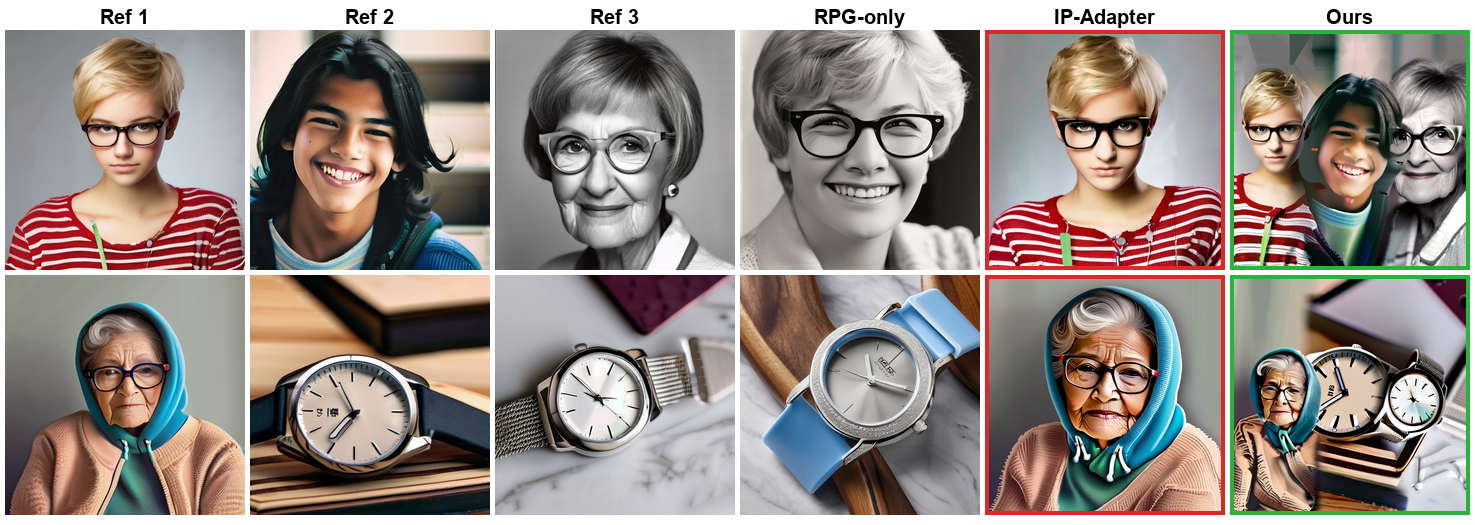
\includegraphics[width=\linewidth]{paper_figures/fig7_three_region.png}
  \caption{%
    \textbf{Three-region generalisation ($N{=}3$).}
    The construction extends to three simultaneous reference concepts
    without modification.  IP-Adapter (global) is conditioned on one
    reference and renders it alone, so the other two concepts are absent.
    Sub-canvas compositing places all three, and the quantitative form of
    that observation is the $N{=}3$ column of Table~\ref{tab:binding}
    ($0.898$ against $0.800$, $p{=}0.0001$).
    The second row also shows the failure the geometry does not prevent:
    with one person and two similar objects the person is composed inside a
    region narrower than a portrait wants, and is rendered at a scale that
    does not match the objects beside it.  Region width is fixed by the
    planner's split ratio and is not adapted to what each region contains
    (Section~\ref{sec:limitations}).
  }
  \label{fig:three_region}
\end{figure}

The construction imposes no upper bound on $N$: the MLLM planner assigns one
reference per region, and the $N$ sub-canvases $\{\Omega_i\}$ partition the
latent, each denoised by its own single-concept adapter pass and fused by
Eq.~\ref{eq:fuse}.  Fig.~\ref{fig:three_region} shows $N{=}3$ person
samples from Mixed-Eval-v1: the per-region isolation holds, whereas global
injection produces an indistinct blend across all three regions.

Whether it keeps holding is a measurement rather than a corollary, and the
structural argument runs in our favour: a sub-canvas is denoised in its own
window, so a region's problem does not depend on how many other regions
exist, whereas a trained layout-conditioned model has no such guarantee.  We
tested it.  \emph{Scaling-Bench} extends the same task to $N\in\{4,5,6\}$
with 30 samples per region count (90 total, 10 per category per count),
scored with the region-level binding accuracy of Section~\ref{sec:binding}.
That metric is the one instrument here that stays interpretable as $N$ grows,
since it is internal to a single image and its chance level $1/N$ is known
exactly.

\begin{table}[htbp]
\centering
\caption{%
  \textbf{Region-level binding accuracy against region count.}
  Scaling-Bench, 30 samples per $N$; the $N{=}2,3$ columns are the
  Mixed-Eval-v1 numbers of Table~\ref{tab:binding}, repeated for continuity.
  $\Delta$ and $p$ compare our default ($\tau{=}0.7$) against MS-Diffusion,
  paired and two-sided; the $\tau{=}0.5$ row is kept to separate the release
  point's contribution from the method's.  Both methods stay above chance at
  every $N$, and the gap between them grows monotonically with the number of
  regions, from $+0.006$ at two to $+0.194$ at six.%
}
\label{tab:scaling}
\resizebox{\columnwidth}{!}{%
\begin{tabular}{lccccc}
\toprule
$N$ & 2 & 3 & 4 & 5 & 6 \\
\midrule
chance               & 0.500 & 0.333 & 0.250 & 0.200 & 0.167 \\
MS-Diffusion         & 0.967 & 0.871 & 0.725 & 0.600 & 0.439 \\
Ours ($\tau{=}0.5$)  & --- & --- & 0.808 & 0.700 & 0.539 \\
\textbf{Ours} ($\tau{=}0.7$) & \textbf{0.973} & \textbf{0.902} & \textbf{0.825}
                     & \textbf{0.713} & \textbf{0.633} \\
\midrule
$\Delta$ ($\tau{=}0.7$) & $+$0.006 & $+$0.031 & $+$0.100 & $+$0.113
                     & $+$0.194 \\
$p$                  & 0.66 & 0.18 & 0.060 & 0.020 & $<$0.001 \\
\bottomrule
\end{tabular}%
}
\end{table}

The structural argument survives, and it is the clearest result in the
paper's favour.  The two methods do not degrade at the same rate: least
squares over $N{=}2\ldots6$ gives $-0.133$ accuracy per added region for
MS-Diffusion against $-0.087$ for ours, a third slower.  The gap grows
monotonically---$+0.006$, $+0.031$, $+0.100$, $+0.113$, $+0.194$---and
becomes significant where it matters most, at $N{=}5$ ($p{=}0.020$) and
$N{=}6$ ($p{<}0.001$), the region counts at which a trained
layout-conditioned model is closest to chance.  At six regions MS-Diffusion
retains $+0.272$ above chance and we retain $+0.466$.

This is what the sub-canvas construction was supposed to buy and, at $768$,
did not.  We report the earlier result because the reason for the difference
is instructive.  A sub-canvas is denoised at the size of its own region, so
at $N{=}6$ on a $768$ canvas each pass runs on a $128$-pixel-wide strip, far
outside the range SDXL was trained on; at $1024$ the same strip is $171$
pixels.  What limits the construction at high $N$ is therefore not the
per-region independence but the resolution that independence leaves each
region, and a backbone evaluated below its native size hides exactly the
advantage the construction is meant to have.  A trained model that reasons
over the whole canvas has no such floor, which is why it loses less from the
smaller canvas and gains less from the larger one.

\begin{figure}[htbp]
  \centering
  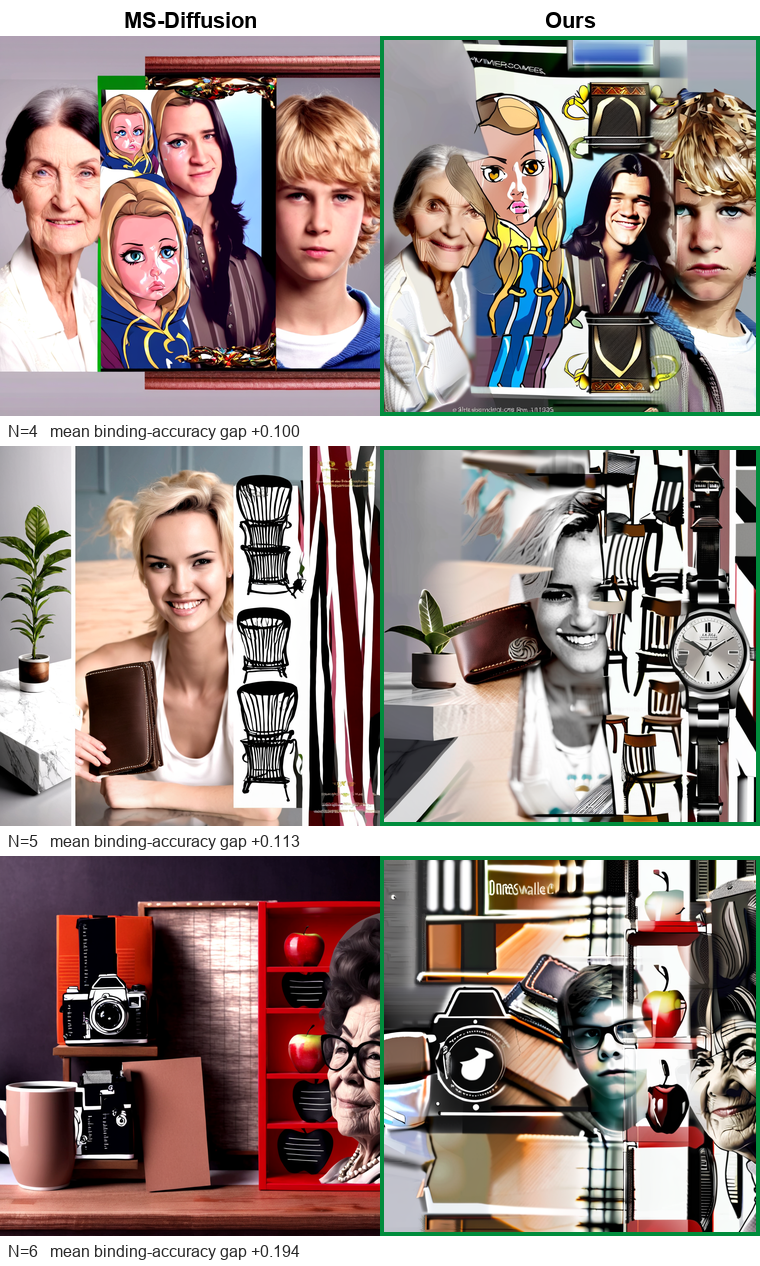
\includegraphics[width=\linewidth]{paper_figures/fig12_scaling.png}
  \caption{%
    \textbf{What the scaling advantage does and does not look like.}
    One sample per region count, chosen by a fixed rule: within each count we
    show the sample whose binding-accuracy gap is closest to the mean gap for
    that count, so the row is typical of the measured difference rather than
    its best case.
    The measured advantage is real---our regions hold the concepts they were
    assigned more often---but the figure shows what the number does not: at
    $N\!\ge\!4$ neither method produces an image a user would keep.  Ours
    fragments into strips with visible stylistic discontinuities; MS-Diffusion
    stays more photographic while binding fewer regions correctly.  Part of
    the disorder is the benchmark's, since Scaling-Bench draws its references
    from the Mixed-Eval-v1 pool whose styles are uncontrolled
    (Section~\ref{sec:exp}), and part is the method's.  We report the figure
    beside the table because the table alone would overstate the result.%
  }
  \label{fig:scaling_visual}
\end{figure}

\noindent\textit{The advantage is in placement, not in usable images.}
Fig.~\ref{fig:scaling_visual} puts the three region counts beside each
other, and it qualifies the result above in a way the table cannot.  At
$N\!\ge\!4$ neither method produces an image that would survive any practical
use: ours breaks into strips with visible stylistic seams, MS-Diffusion holds
a more photographic composition while placing fewer concepts where they
belong.  What Scaling-Bench establishes is therefore that the sub-canvas
construction keeps assigning concepts to their regions further into a regime
where both methods have already stopped producing usable output---a statement
about the mechanism's degradation, not a claim that the method is useful at
six regions.  The practical range of the method, on this evidence, is the
$N\!\le\!3$ of Mixed-Eval-v1.

\noindent\textit{The release point contributes little of this.}
Holding resolution fixed, moving $\tau$ from $0.5$ to $0.7$ is worth
$+0.017$ at $N{=}4$ ($p{=}0.48$), $+0.013$ at $N{=}5$ ($p{=}0.70$) and
$+0.094$ at $N{=}6$ ($p{=}0.001$).  Only the last is significant and we
report it uncorrected for three tests, so the honest reading is that the
release point costs little at any region count rather than that it helps at
high ones.  The separation above is the geometry's, not the schedule's.

\begin{figure}[H]
  \centering
  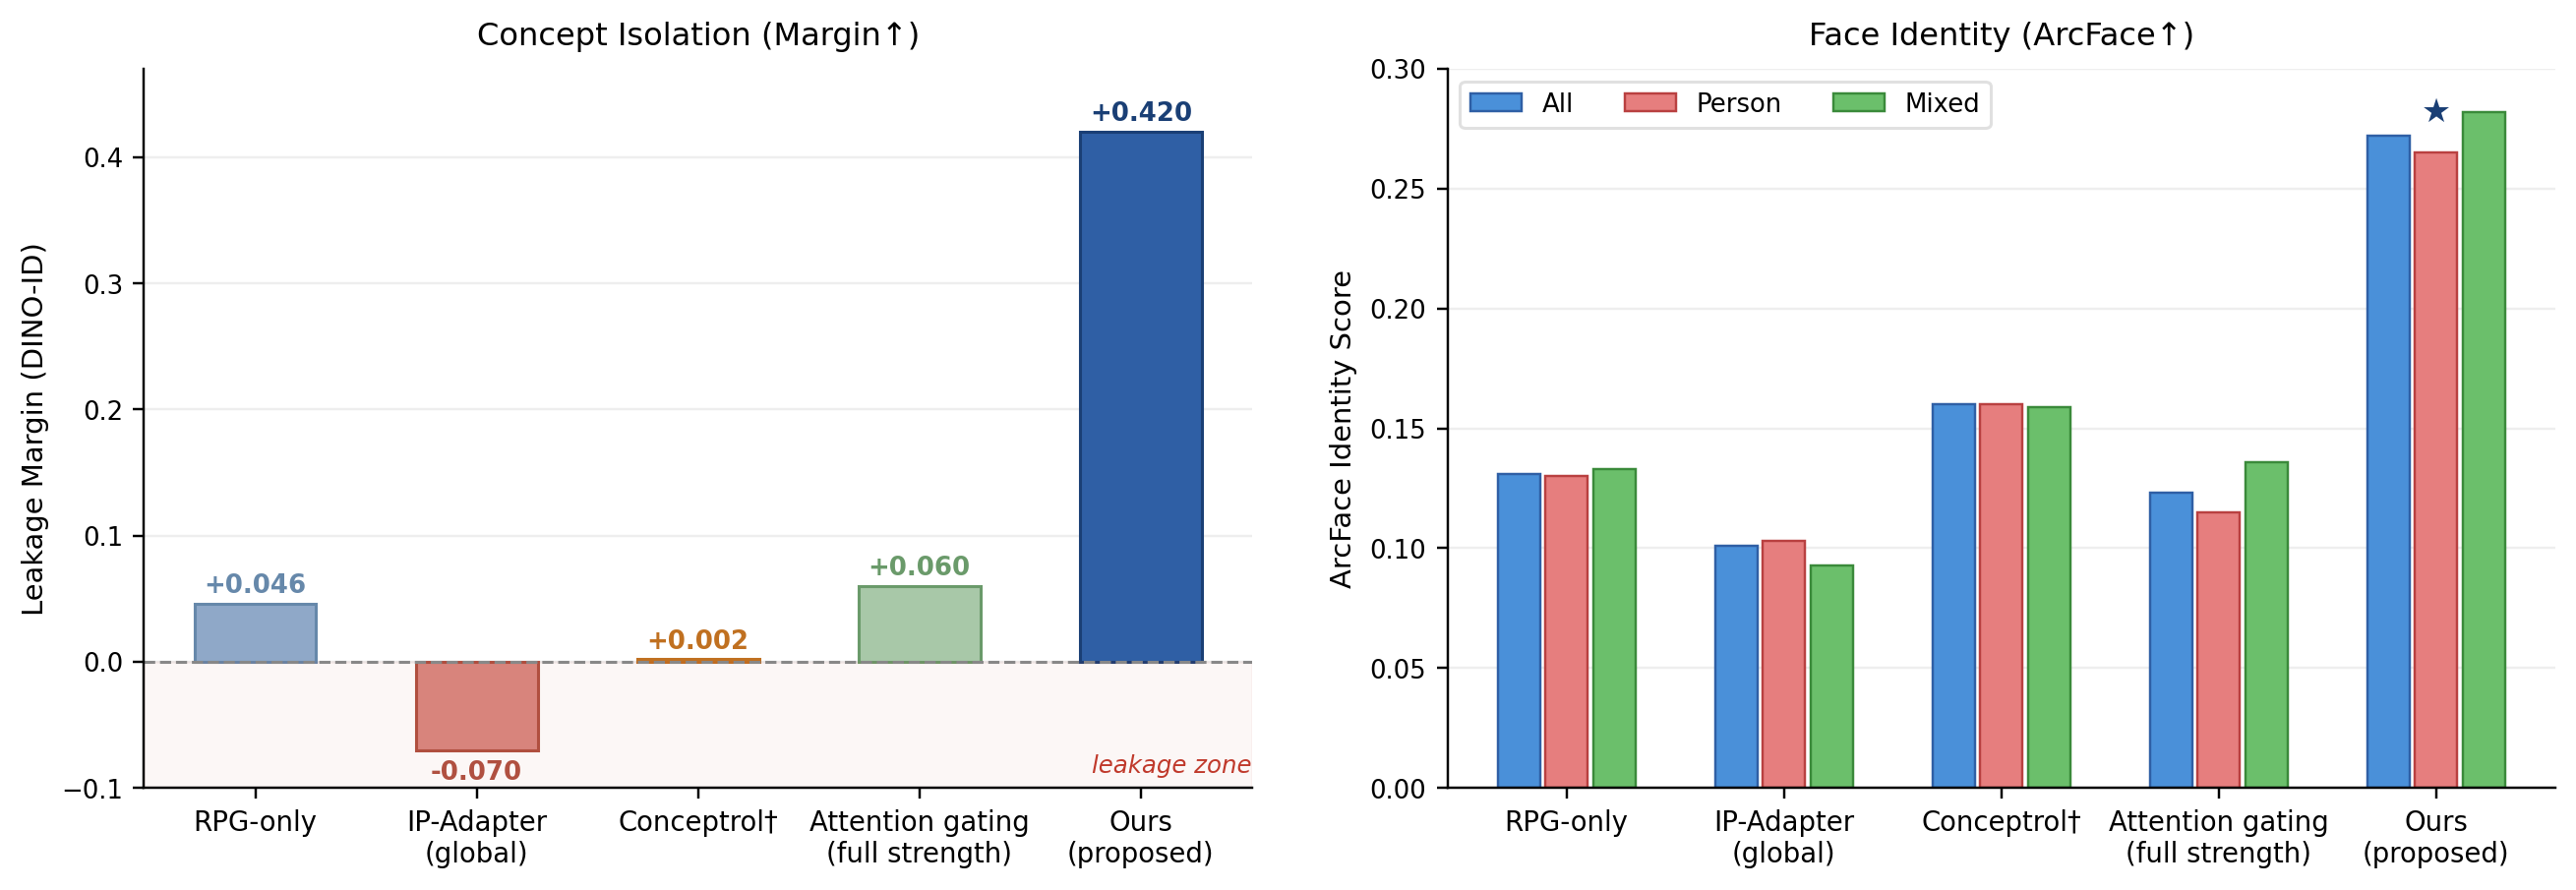
\includegraphics[width=\linewidth]{paper_figures/fig8_metrics_chart.png}
  \caption{%
    \textbf{Metric comparison.}
    Left: Leakage Margin.  Global IP-Adapter falls below zero (leakage zone,
    red shading); Conceptrol$^{\dagger}$ and attention gating at full strength
    sit at essentially zero, i.e.\ each region crop matches the wrong reference
    as well as its own; only sub-canvas compositing separates the concepts.
    Right: ArcFace identity by category.  Conceptrol transfers more face
    identity than the other baselines but, as the Margin shows, into a single
    merged subject rather than two.
  }
  \label{fig:metrics_chart}
\end{figure}
%%ENDSUPP

%%SUPP{failure}
\subsection{Failure Case Analysis}
\label{sec:failure}

Despite strong average performance, our method exhibits recurring
failure modes that reveal the limits of training-free spatial conditioning.
We categorise the worst-performing samples (DINO-ID $< 0.16$) from
Mixed-Eval-v1 into four patterns:

\noindent\textbf{(F1) Crowded three-region layouts.}
When $N{=}3$ equal-width regions are used, each strip is only
$\sim$341\,px wide at 1024\,px resolution.
The IP-Adapter cross-attention guidance spreads across the narrow strip
and cannot fully suppress leakage from adjacent regions.
Sample \texttt{mixed\_3r\_039} (mug $\mid$ teenager $\mid$ plant)
achieves DINO-ID\,=\,0.107 and Margin\,=\,$-$0.133—the worst leakage
in the dataset.

\noindent\textbf{(F2) Visually generic objects.}
Everyday objects such as apples, mugs, and books produce nearly
identical DINOv2 embeddings across different instances.
Even when the generated image renders the correct object category,
the metric registers low identity because DINOv2 encodes instance-level
texture rather than category membership.
Samples \texttt{object\_3r\_032} and \texttt{object\_3r\_047}
(apple/watch/mug and apple/book/plant, respectively) illustrate this:
the model generates plausible objects, but the embedding comparison
yields ID $< 0.16$.

\noindent\textbf{(F3) Contradictory textual descriptions.}
Some sub-prompts assign conflicting attributes to one subject---``long black
hair'' and ``short blonde hair'' in \texttt{person\_3r\_029}, for
instance---and both the text encoder and the adapter respond with a blended
or incoherent appearance (DINO-ID\,=\,0.150).  The fault is ours rather than
the planner's: it originates in Mixed-Eval-v1's prompt construction, which
draws two attributes without excluding pairs from the same group, and affects
$11.2\%$ of person sub-prompts (Section~\ref{sec:exp}).  The planner
propagates the contradiction faithfully.  We keep these samples in every
table because removing them after the fact would be selection on the outcome,
and because the contradiction is identical for every method compared.

\noindent\textbf{(F4) Face identity in narrow person strips.}
Three-person layouts force each face into a $\sim$341\,px strip.
ArcFace detection success drops below 50\% in these cases, and even
when faces are detected, the limited spatial extent weakens the
IP-Adapter conditioning signal relative to the background.
\texttt{person\_3r\_049} achieves DINO-ID\,=\,0.150 and
Margin\,=\,$-$0.077.

These failure modes suggest that future work should focus on
adaptive region sizing guided by concept salience, and reference
denoising strategies that increase robustness to view-angle variation.

\noindent\textbf{Single-concept identity methods do not extend to this
setting.}
We ran InstantID~\cite{wang2024instantid} at $768$ before settling on the
native-resolution protocol and do not carry the row forward, but the failure
is worth one sentence because it is structural rather than incidental: the
method derives face keypoints from \emph{one} reference and applies them as a
ControlNet condition to the \emph{entire} canvas, so in a two-person layout a
single face geometry is imposed over both regions and neither crop passes
ArcFace detection on any of the 150 samples.

% ============================================================
%%ENDSUPP

%%SUPP{cost}
\subsection{Computational Efficiency}
\label{sec:efficiency}
% ============================================================

Table~\ref{tab:timing} reports per-image denoising time and peak GPU
memory on a single NVIDIA RTX\,5080 (16\,GB) at $768\!\times\!768$, 30
DPM-Solver++ steps.  Every configuration is measured with the
\emph{identical} inline sampler, no CPU offloading, and the VAE decode
excluded, so the numbers are directly comparable and reflect the
denoising loop alone.  A single full-canvas conditioned pass---the
per-step cost of global IP-Adapter---is the natural unit of comparison;
region-planning baselines such as RPG-only and Conceptrol perform at
least one such pass plus their own regional or masking overhead.

\begin{table}[htbp]
\centering
\caption{Inference cost (RTX\,5080\,16\,GB, $768\!\times\!768$, 30
         DPM-Solver++ steps, seed 42; \texttt{time.perf\_counter}, 5
         timed runs after 2 warm-ups, identical inline sampler, no CPU
         offload, VAE decode excluded).}
\label{tab:timing}
\resizebox{\columnwidth}{!}{%
\begin{tabular}{lcc}
\toprule
Method & s\,/\,image & $\times$\,IP-global \\
\midrule
IP-Adapter (global)      & \textbf{9.46} & 1.00$\times$ \\
\textbf{Ours}            & 9.88 & 1.04$\times$ \\
MS-Diffusion             & 11.92 & 1.26$\times$ \\
RPG-only                 & 15.64 & 1.65$\times$ \\
Attention gating         & 16.00 & 1.69$\times$ \\
Conceptrol               & 17.22 & 1.82$\times$ \\
\bottomrule
\end{tabular}%
}
\end{table}

Sub-canvas compositing evaluates the UNet once per region per step, but
each pass runs on a sub-window narrower than the full canvas, so cost
grows \emph{sublinearly} in the number of regions $N$: two regions cost
$1.4\times$ a single full-canvas pass rather than $2\times$, and three
cost $2.0\times$ rather than $3\times$.  Peak memory stays flat at
$9.5$\,GB across $N$---only one sub-canvas is resident at a time and the
footprint is dominated by the fixed SDXL and adapter weights---so the
method adds concepts within the 16\,GB budget without the memory
blow-up of batching $N$ full-resolution images.

% ============================================================
%%ENDSUPP

%%SUPP{trained}
\subsection{Comparison with Training-Based Methods}
\label{sec:training_compare}

Our method targets the \emph{zero-shot} setting: given only inference-time
reference images, it produces personalised multi-concept images without
any per-concept optimisation.
Training-based methods—DreamBooth~\cite{ruiz2023dreambooth},
Custom~Diffusion~\cite{kumari2023multi}, and
Mix-of-Show~\cite{gu2023mix}—generally achieve higher fine-grained
identity fidelity by embedding specific concepts into model weights.
However, they require per-concept (or per-concept-pair) fine-tuning
before inference, which precludes use when reference images arrive at
test time.
Table~\ref{tab:training_cost} summarises the practical trade-off.

\begin{table}[htbp]
\centering
\caption{%
  Training cost vs.\ capability comparison.
  ``Inference-time reference'' = method accepts unseen reference
  images without retraining.
  $^{*}$FreeCustom is tuning-free but additionally requires an external
  segmentation model to obtain per-concept masks.
}
\label{tab:training_cost}
\resizebox{\columnwidth}{!}{%
\begin{tabular}{lccccc}
\toprule
Method & Training & Per-concept time & Multi-concept & Inference-time ref & Backbone \\
\midrule
DreamBooth~\cite{ruiz2023dreambooth}   & Full UNet   & $\sim$30\,min & \texttimes & \texttimes & SD \\
Custom Diffusion~\cite{kumari2023multi}& Key layers  & $\sim$30\,min & Partial     & \texttimes & SD \\
Mix-of-Show~\cite{gu2023mix}           & LoRA / concept & $\sim$20\,min & \checkmark  & \texttimes & SD \\
\midrule
MC$^2$~\cite{mc2_2025}                 & Per-concept models & $\sim$20\,min & \checkmark & \texttimes & SD \\
LaTexBlend~\cite{latexblend2025}       & Per-concept bases  & $\sim$20\,min & \checkmark & \texttimes & SD \\
LoRAShop~\cite{dalva2025lorashop}      & LoRA / concept & $\sim$20\,min & \checkmark & \texttimes & Flux \\
FreeCustom~\cite{freecustom2024}       & None        & ---           & \checkmark  & \checkmark & SD\,1.5$^{*}$ \\
\midrule
MS-Diffusion~\cite{wang2025msdiffusion}& Corpus, once & \textbf{---} & \checkmark & \checkmark & SDXL \\
FastComposer~\cite{xiao2024fastcomposer}& Corpus, once & \textbf{---} & \checkmark & \checkmark & SD \\
XVerse~\cite{chen2025xverse}           & Corpus, once & \textbf{---} & \checkmark & \checkmark & Flux \\
\midrule
IP-Adapter (global)                    & None        & ---           & \checkmark  & \checkmark & SDXL \\
\textbf{Ours}                          & \textbf{None} & \textbf{---} & \checkmark  & \checkmark & SDXL \\
\bottomrule
\end{tabular}%
}
\end{table}

\noindent
The distinction that matters is not training in general but \emph{per-concept}
training.  Methods in the first block bake each concept into weights before
inference, so a reference photograph first seen at test time cannot be used at
all; quantitative comparison against them would confound the mechanism under
study with a strictly easier problem setting, and we do not attempt it.
Methods in the second block are trained once on a subject-annotated corpus and
are then zero-shot exactly as we are.  Those \emph{are} directly comparable,
and the strongest of them that targets our layout-conditioned setting on our
backbone, MS-Diffusion, is evaluated head-to-head in Table~\ref{tab:main}
under a matched protocol.  On that benchmark we lead it on identity,
placement and isolation and trail it on text alignment
(Section~\ref{sec:main_results}), and we present both halves, including the
layout convention under which the isolation result reverses.  What our method
offers besides is the absence of a subject-annotated training corpus and a
lower cost per image ($9.88$\,s against $11.92$\,s); what the comparison
establishes for the argument of this paper is that
the separation both methods achieve is unreachable by the training-free
attention-gated route, whether it is bought with supervision or with a change
of injection site.

\noindent\textit{On recent multi-concept methods.}
The 2025 multi-concept literature is dominated by two families, neither
of which yields a like-for-like baseline in our setting.
MC$^2$~\cite{mc2_2025} and LaTexBlend~\cite{latexblend2025} \emph{compose
pre-trained single-concept models}: every concept must first be embedded
into weights by a per-concept optimisation run, so they inherit the
training-based limitation above and cannot consume a reference photograph
that first appears at test time.
FreeCustom~\cite{freecustom2024} is genuinely tuning-free, but couples a
multi-reference self-attention mechanism to an SD\,1.5 backbone and
additionally requires an external segmentation network to produce the
per-concept masks it filters with; differences in backbone capacity and
mask supervision would dominate any direct metric comparison against our
SDXL pipeline.
We therefore compare against the mechanism these methods share---confining
identity \emph{inside} the attention operator---rather than against their
individual implementations, which is exactly the attention-gating ablation
of Table~\ref{tab:ablation}.  That ablation is backbone-, planner- and
seed-matched to our method, and so isolates the design choice under study
instead of conflating it with backbone differences.

% ============================================================
%%ENDSUPP

\subsection{Limitations}
\label{sec:limitations}

The method depends on an external MLLM for planning, at API cost and
latency.  Its rectangles are assumed non-overlapping, so concepts that
genuinely overlap are out of reach, and region width follows the planner's
split ratio rather than what each region has to contain---a portrait and a
small object placed side by side get equal width and are rendered at
mismatched scales (Fig.~\ref{fig:three_region}).  Strongly overlapping
concepts, extreme lighting differences between references and non-frontal
poses remain hard, and performance degrades on crowded three-region layouts
and on visually generic objects (Section~\ref{sec:failure}).

Resolution is a limitation we measured rather than anticipated.  A sub-canvas
is denoised at the size of its own region, so the construction inherits a
floor the backbone imposes: at $N{=}6$ on a $768$ canvas each pass runs on a
$128$-pixel strip, and the advantage over a trained layout-conditioned model
disappears there ($-0.134$ against $-0.137$ accuracy per added region, where
at $1024$ it is $-0.087$ against $-0.133$).  The method needs the backbone's
native resolution to show what it can do, and costs $15.8$\,GB to run there
(Section~\ref{sec:scaling}).

\noindent\textit{Our regions tile the canvas, which costs isolation and text
alignment.}
The planner emits adjacent, full-height strips that partition the entire
image, so no part of the canvas is ever denoised as background.  Two
consequences follow: the text-alignment axis on which MS-Diffusion leads us,
and the isolation lead that reverses once the baseline is handed its own
layout convention instead of ours.  Concept isolation suffers because neighbouring
regions meet each other directly rather than across a background gap: the
reported MS-Diffusion configuration uses tighter, non-adjacent boxes, and
handed our planner's strips instead it loses $0.112$ Margin
(Section~\ref{sec:main_results})---more than the entire gap between the two
methods.  Text alignment suffers for a related reason: a region with no
background of its own reproduces the reference's context along with its
subject, so a prompt that places the subjects in a new setting is only
partly honoured.  This is clearest on DreamBench-2, where the references
are photographs carrying their own scenes and the released global phase is
too short to replace them.  It also bounds how our identity numbers should
be read---similarity to a reference is raised by reproducing its
background, and neither DINO-ID nor the reference-response measure of
Section~\ref{sec:refresponse} separates transferring a subject from copying
the photograph it came in.

The obvious repair is to give the layout a background region, and it does not
work.  We ran the method unchanged except that each region is shrunk to a
tight, non-adjacent box ($80\%$ of its strip's width, vertical band
$[0.15,0.85]$, the shape MS-Diffusion's released examples use) and everything
outside the boxes is carried by one full-canvas pass on a scene-only prompt
with the adapter switched off.  On 30 samples at $\tau{=}0.7$ it is worse on
all three axes, including the two it was meant to repair: DINO-ID $-0.116$
($p{<}0.001$), Margin $-0.106$ ($p{<}0.001$), CLIP-T $-0.007$ ($p{=}0.010$).
Scoring it on its own boxes rather than on the planner's strips does not
rescue it ($0.665$ against $0.690$ DINO-ID).  The damage is four times larger
on person regions than on object regions ($-0.197$ against $-0.047$ DINO-ID),
and the images say why: a person-sized rectangle whose interior disagrees with
its surroundings is rendered as a framed portrait or a standee, because that
is what such a rectangle usually is in a photograph.  Objects fare better
because a small object on a shared surface is a composition the model already
knows.

Two further repairs fail for the same underlying reason and are worth
recording.  Telling each sub-canvas that it is a \emph{crop} of the full
canvas rather than a complete image---SDXL's own crop conditioning, which
ought to make the regions agree on one framing---costs $0.083$ DINO-ID
($p{<}0.001$, worse on 25 of 30 samples), because the subject is then composed
for the full canvas and falls largely outside its own window.  Appending a
shared scene clause to every sub-prompt changes the outputs almost not at all.

\begin{table}[htbp]
\centering
\caption{%
  \textbf{Thirteen attempts to remove the panel structure.}  Identity cost is
  the paired DINO-ID difference from the method as reported, on the subset each
  variant was run over; a dash means the outputs were unchanged to three
  decimals.  \emph{Step} is the low-frequency boundary ratio defined at the end of this
  section, for which $1.10$ is the method as reported,
  $1.06$ is the same geometry driven by text alone, and $1.37$ is a collage.
  The first nine attempts span three mechanisms---what the regions are
  (geometry), what each pass can see (receptive field), and what conditions or
  post-processes them---and no member of any group both preserves identity and
  removes the boundary.  The last three act on a fourth thing, what the
  adapter is shown, and they do remove it.%
}
\label{tab:repairs}
\resizebox{\columnwidth}{!}{%
\begin{tabular}{llccl}
\toprule
Attempt & Mechanism & $\Delta$ DINO & Step & Outcome \\
\midrule
Crop size-conditioning        & field    & ---      & ---   & unchanged \\
Shared scene clause           & text     & ---      & ---   & unchanged \\
Quantised fusion mask         & field    & $+0.004$ & 1.30  & step grows \\
Whole-canvas harmonisation    & post-hoc & $-0.012$ & 1.10  & boundary intact \\
Larger sub-canvas overlap     & field    & $-0.043$ & 0.98  & step falls, look unchanged \\
Feathered attention box       & field    & $-0.128$ & ---   & worse on both axes \\
Subject-silhouette weights    & geometry & $-0.189$ & ---   & cut-out edges \\
Tight boxes, global background& geometry & $-0.204$ & ---   & cut-out edges \\
Per-region context rebuild    & post-hoc & $-0.230$ & ---   & worse coherence \\
\midrule
Segmented refs, grey ground   & reference& $-0.035$ & 1.06  & step gone, scene gone \\
Segmented refs, shared ground & reference& $-0.033$ & 1.02  & step gone, scene defocused \\
\quad + feathered alpha       & reference& $-0.019$ & 1.02  & least costly repair \\
\midrule
Latent token replacement      & site     & $+0.043$ & ---   & pastes the reference \\
\bottomrule
\end{tabular}%
}
\end{table}

Table~\ref{tab:repairs} collects thirteen attempts, of which the following are
the informative ones.  A fourth attempt worked as designed.  Shrinking
each region to a tight box, leaving the area outside the boxes to a single
global pass, and conditioning that pass on the sample's own prompt with its
subject nouns removed---so that the background pass paints the setting and
not the people who belong in the boxes---does put the prompted scene on the
canvas: on 30 DreamBench-2 samples CLIP-T rises by $+0.028$
($p{<}0.001$), closing half the gap to the text-only baseline
($-0.057\!\to\!-0.028$).  It costs DINO-ID $-0.204$ and Margin $-0.237$,
both $p{<}0.001$.  The identity given up is seven times the text alignment
bought, and the reason is visible in the construction: the background can
only become global by making each subject's window smaller, and a smaller
window carries less of its subject.

Taken together the first nine say something narrower than a list of
failures.  Within noise-level fusion, what a region can write is bounded by
the share of the canvas its prediction is allowed to occupy, and every scheme
that hands part of the canvas to a shared pass takes that share away: the
cost tracks how much of the \emph{subject} is given up, which is why
silhouette weights ($-0.189$) cost nearly what a shrunken box costs
($-0.204$) while covering far less area.  Softening the boundary does not
help either---feathering the attention box loses identity and isolation
together---and a post-hoc pass weak enough to preserve the image preserves
the boundary with it.  The one variant that improves every metric does so by
ceasing to generate (Section~\ref{sec:refresponse}).

%%SUPP{panel}
\noindent\textit{The control we should have run first, and the conclusion it
overturns.}
Nine failures spread across geometry, receptive field, and post-processing
invite the conclusion that the panel structure is intrinsic to noise-level
fusion.  An earlier draft of this analysis drew exactly that conclusion.  It
is wrong, and the control that refutes it is the cheapest one available.  We
ran the method with the same regions, the same overlap, the same schedule and
the same fusion rule, changing one thing: the adapter scale is set to zero, so
each sub-canvas is driven by its text prompt alone.  The boundary step is
$1.059$, against $1.103$ for the method as reported and $1.37$ for a collage,
on the same 30 samples.  Sub-canvas fusion applied to text-conditioned regions
leaves no visible seam.  What leaves one is the references: two photographs
taken in different places, transferred whole by the adapter---background
included---and each reproduced faithfully by the pass that receives it.  The
boundary is where two reproduced scenes meet.

This reattribution predicts its own repair, and the prediction holds.
Segmenting each subject and compositing it onto a common ground before
encoding gives the two passes nothing left to disagree about, and the step
returns to the text-only floor: $1.062$ on flat grey, $1.017$ on a shared
defocused backdrop.  The dose behaves as the account requires---blurring that
shared backdrop by $24$ pixels rather than $48$ leaves enough of the original
scene legible for the two passes to keep disagreeing, and the step stays at
$1.096$, statistically indistinguishable from the method as reported.  The
price is a small but real loss of identity, $-0.035$ and $-0.033$ DINO-ID
respectively (both $p{<}0.01$), because the discarded background was carrying
part of what DINO was matching on.

Most of that identity loss is recoverable, and the way it is recovered
confirms the mechanism a second time.  A binary silhouette composites the
subject onto the ground as a cut-out, and the adapter transfers the cut-out
edge along with the subject; blurring the segmentation alpha by $24$ pixels so
that the subject fades into the ground instead recovers two fifths of the
loss, to $-0.019$ DINO-ID and $-0.027$ Margin, while holding the step at
$1.016$.  Against the unfeathered variant the identity gain is $+0.014$
($p{=}0.046$).  The best repair we have is therefore a preprocessing step on
the references alone: segment, composite onto one defocused ground, feather
the seam.  It touches neither the fusion rule nor the layout, which is the
point.

\noindent\textit{When it works and when it cannot.}
The repair is bounded by what segmentation can extract.  Where each reference
contains a subject with a silhouette---a person, an animal, an object---the
two grounds agree and the boundary closes.  Where a reference \emph{is} a
scene, as with our stained-glass and multi-panel character-sheet references,
there is no subject to lift off it, the segmenter returns most of the frame,
and the panel survives every variant above.  That is a limitation of the
diagnosis and also a small confirmation of it: the boundary persists in
exactly the cases where the two references still carry incompatible contexts
after the repair.

Two honest qualifications.  The $1.017$ figure sits \emph{below} the
text-only floor, and it should: with the same blurred image behind both
subjects the low-frequency field is continuous by construction, so on this
one variant the measure is partly reporting what we built rather than what
was generated.  And a defocused ground is not the prompted scene---the seam
is gone, but so is the setting, which is the same trade
Section~\ref{sec:why_gating_fails} reaches from the other direction.  We
therefore report the segmented-reference variants as a diagnosis that
localises the cause and as an optional preprocessing step with a measured
price, not as a replacement for the method whose numbers this paper reports:
every comparison in Sections~\ref{sec:main_results}--\ref{sec:scaling} is run
without it, so that what is compared across methods is the generation
procedure and not our choice of segmenter.  The
two directions that would keep the scene are outside this paper's setting:
token replacement in a backbone whose tokens carry semantics, which requires
a DiT, and a trained grounding module, which requires the corpus whose
absence is the point of a training-free comparison.
%%ENDSUPP

\subsection{Identity in the text stream}
\label{sec:textstream}

Every configuration above puts identity into a branch running alongside the
text, and a CLIP image embedding is not a description of who the subject is
but of a photograph: it carries that photograph's pose, framing and background
with it.  The branch cannot supply the first without imposing the rest---turn
it up and the composition collapses towards the reference's bust framing, turn
it down and no identity arrives---and inside RPG no setting delivers identity
at all (Table~\ref{tab:cascade}).

A different site avoids the bundling.  PhotoMaker~\cite{li2024photomaker}
fuses an identity into the \emph{text token} of the subject's class noun, so
there is no second branch and nothing competes with the prompt for framing or
pose.  Composing it with RPG needs no new machinery: RPG already encodes each
region's prompt into its own $77$-token block and routes that block's
attention to that region's pixels, so fusing subject $i$'s identity into
region $i$'s class noun makes the identity regional for free.  No mask, no
gating, no intersection.

\begin{table}[htbp]
\centering
\caption{%
  \textbf{Text-stream identity keeps the prompt's framing.}  Photographic
  human-human pairs, $24$ samples, prompted as medium shots.  ArcFace does not
  move with framing; face area shows what the prompt asked for ($9.48\%$) and
  what each configuration delivered.  The fusion adds identity without moving
  the framing; PhotoMaker's LoRA moves the framing without adding identity.%
}
\label{tab:textstream}
\resizebox{\columnwidth}{!}{%
\begin{tabular}{lccc}
\toprule
Configuration & ArcFace & Faces/img & Face area \\
\midrule
RPG, text only                    & $+$0.014 & 1.96 & \phantom{0}9.48\% \\
\midrule
Fusion off, LoRA on               & $+$0.004 & 1.42 & 22.13\% \\
Fusion on,  LoRA on               & $+$0.120 & 1.67 & 20.50\% \\
\midrule
Fusion $w{=}1.0$, no LoRA         & $+$0.165 & 1.96 & 10.04\% \\
Fusion $w{=}1.5$, no LoRA         & $+$0.225 & 2.00 & 10.54\% \\
\textbf{Fusion $w{=}2.0$, no LoRA}& \textbf{$+$0.244} & 1.96 & \textbf{11.43\%} \\
\midrule
Sub-canvas (ours, as reported)    & $+$0.254 & 2.04 & 18.31\% \\
\bottomrule
\end{tabular}%
}
\end{table}

Table~\ref{tab:textstream} separates two things that the released checkpoint
ships together.  PhotoMaker also provides a LoRA, trained on portraits.  With
the fusion switched off the LoRA alone scores at chance ($+0.004$) while
pulling the framing from the prompt's $9.48\%$ to $22.13\%$---it carries no
identity and costs the composition.  With the LoRA switched off the fusion
alone reaches $+0.165$ at $10.04\%$, and scales to $+0.244$ at $11.43\%$ when
the fused token is extrapolated ($w{=}2$).  Identity comes from the fusion;
framing damage comes from the LoRA; the two are separable and we keep only the
first.

At $w{=}2$ the identity is level with the sub-canvas method of this paper
($+0.244$ against $+0.254$) at $62\%$ of the face area---that is, in a medium
shot rather than a pair of busts.  Both subjects render ($1.96$ faces per
image), which the regional ArcFace adapter of Section~\ref{sec:framing} could
not achieve, and references whose faces no detector finds still work, because
the encoder is CLIP-based rather than detection-based.

\begin{figure*}[t]
  \centering
  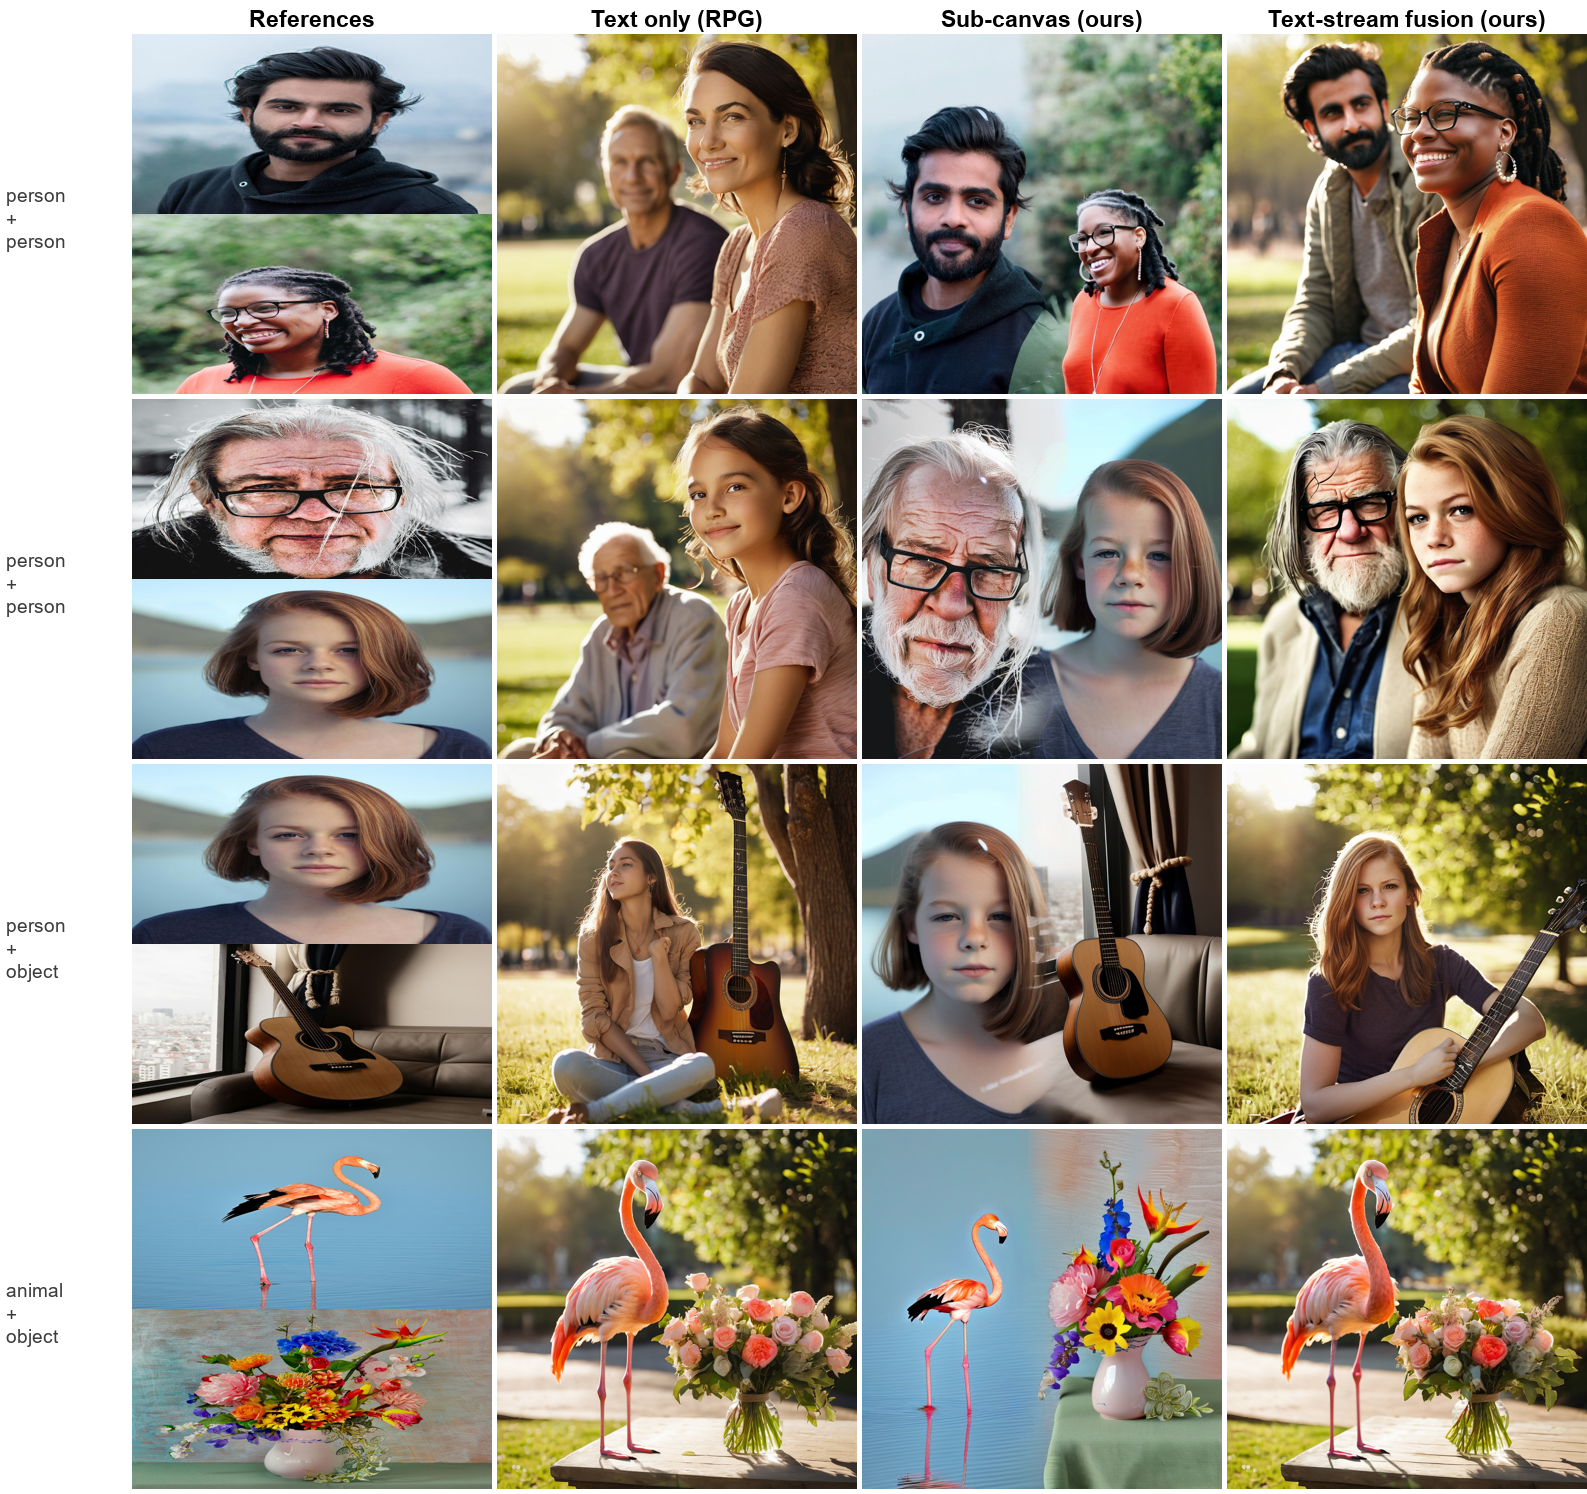
\includegraphics[width=\linewidth]{paper_figures/fig13_textstream.png}
  \caption{%
    \textbf{What the text-stream route delivers, and where it stops.}
    All columns use the same medium-shot prompt and the same seed.  For
    \emph{person} subjects (top two rows) the fusion puts both references into
    the scene the prompt describes, at the scale the prompt asked for, while
    sub-canvas compositing recovers the same identities as a pair of busts.
    For the \emph{object} region of row three the fusion changes nothing: the
    guitar is a guitar, not \emph{that} guitar, and only sub-canvas reproduces
    the reference instrument.  Row four is the boundary case---neither subject
    is a person, so the fusion is skipped entirely and the output is the
    text-only render.  PhotoMaker's encoder is trained on faces, and the method
    inherits exactly that scope; object and animal fidelity remains the
    sub-canvas method's.
  }
  \label{fig:textstream}
\end{figure*}

\noindent\textit{The fusion belongs only where the encoder was trained.}
Applied to every region, the fusion writes something meaningless into
``flamingo'' and ``vase'': on DreamBench-2's animal-object pairs DINO-ID falls
from $0.609$ with text alone to $0.442$.  Restricting it to person-like class
nouns repairs that and improves the rest, since the human half of a mixed pair
still gains.  Fig.~\ref{fig:textstream} shows the same boundary visually.

\begin{table}[htbp]
\centering
\caption{%
  \textbf{DreamBench-2, all $150$ samples, by pair type (DINO-ID).}  H, A and O
  are human, animal and object.  Routing the fusion to person regions only
  returns non-human subjects to the text-only baseline instead of damaging
  them.  CLIP-T is the highest of any identity-carrying method here.%
}
\label{tab:db2_textstream}
\resizebox{\columnwidth}{!}{%
\begin{tabular}{lcccccc}
\toprule
Method & DINO & Margin & CLIP-T & HH & HA & HO \\
\midrule
RPG, text only          & 0.361 & $+$0.280 & \textbf{0.660} & 0.161 & 0.363 & 0.371 \\
Fusion, all regions     & 0.392 & $+$0.315 & 0.643 & 0.327 & 0.455 & 0.356 \\
Fusion, persons only    & 0.457 & $+$0.393 & 0.656 & 0.327 & 0.493 & 0.434 \\
\midrule
MS-Diffusion            & 0.705 & $+$0.640 & 0.639 & 0.674 & 0.664 & 0.712 \\
Sub-canvas (ours)       & \textbf{0.806} & \textbf{$+$0.752} & 0.623
                        & \textbf{0.788} & \textbf{0.823} & \textbf{0.793} \\
\bottomrule
\end{tabular}%
}
\end{table}

\noindent\textit{What this does and does not settle.}
On DINO-ID the text-stream route stays far below the sub-canvas method
($0.457$ against $0.806$), and Section~\ref{sec:framing} says why that
comparison is unsafe: the two frame differently, and DINO-ID moves with
framing.  On the framing-independent measure they are level for human
subjects.  We therefore do not claim the text-stream route as a replacement.
It is the first configuration in this study that delivers identity
\emph{without} taking the composition, and the mechanism---identity in the
tokens the planner already routes, rather than in a branch that competes with
them---is what makes that possible.  Its limits are equally clear: it applies
to subjects whose class the identity encoder was trained on, which here means
people, and object and animal identity remains the sub-canvas method's.

We tried to close that gap by running both sites in one image---the fusion on
person regions, RPG's regional adapter at full strength on the rest, selected
per region.  It does not close: on animal-object pairs, where the adapter is
the only thing carrying identity, DINO-ID moves from $0.611$ to $0.633$
against $0.822$ for sub-canvas, about a tenth of the gap.  The reference
robot is still rendered as a generic robot and the reference guitar as a
generic guitar.  This is the same result as
Table~
ef{tab:cascade}, now for non-human subjects: the attention site does
not carry identity, and pairing it with a site that does for a different class
of subject gives each class only what its own site can deliver.  We therefore
report two operating points rather than one method---text-stream fusion where
the subjects are people and the composition matters, sub-canvas where subject
fidelity matters---and do not claim a configuration that is best at both.

%%SUPP{frontier}
\subsection{The frontier is the backbone's, not the tuning's}
\label{sec:architecture}

Every configuration in this study trades identity against framing, and the
trade is remarkably stable: across four mechanisms and roughly twenty
configurations, more identity arrives only with a larger face, a tighter crop
and a boundary between the regions.  Nothing we tried escaped it.  A reader is
entitled to suspect that a study which fails twenty times has simply not found
the right setting.

Concurrent work names the reason, and it is architectural rather than a matter
of search.  Feng et al.~\cite{feng2026personalize} observe that a diffusion
transformer represents content in tokens whose position is supplied separately,
so a reference's tokens can be injected \emph{without} their positional
information, whereas a U-Net's convolutions entangle content with position and
reproduce the reference's spatial arrangement along with its appearance.  Our
measurements are the U-Net side of exactly that statement.  A CLIP image
embedding fed to IP-Adapter cannot deliver ``who this is'' without also
delivering ``framed like this'': raising the adapter's strength collapses the
prompt's medium shot to the reference's bust ($9.5\% \to 20.5\%$ face area,
Table~\ref{tab:textstream}), and lowering it removes the identity instead.  The
same entanglement explains why sub-canvas compositing scores highest on
identity while sitting closest to a literal paste, and why attention gating
inside RPG recovers no identity at any strength (Table~\ref{tab:cascade}): a
spatial mask can restrict where entangled content lands, but cannot separate
what is entangled.

Read that way, the results here and the DiT results are consistent rather than
competing.  Token replacement is the rung our ladder ends on and could not
climb---on SDXL it improves every metric we report while reproducing the
reference almost exactly (Section~\ref{sec:refresponse})---and on a DiT the
same operation succeeds, with early injection for consistency and late
regularisation for flexibility~\cite{feng2026personalize}.  The regularisation
is aimed at the failure our copy-fidelity check measures.  Work that removes
the pose entanglement without changing backbone does so by training for it:
Qian et al.~\cite{qian2025canvascomposer} disentangle pose and illumination
across subjects with a cross-reference objective, which is not available to a
training-free method.

We therefore state the scope of this paper's negative results precisely.  They
are not evidence that regional personalisation is hard; they are measurements
of what a U-Net's cross-attention can and cannot be asked to do, with the size
of each cost attached.  The text-stream route of
Section~\ref{sec:textstream} is the one configuration that sidesteps the
entanglement without leaving the backbone, and it does so by not using the
image branch at all---which is also why its scope is limited to subjects whose
identity encoder was trained on faces.
%%ENDSUPP

\subsection{What DINO-ID actually measures}
\label{sec:framing}

Every identity number in this paper, and in the literature it compares
against, is a similarity between a reference and a crop of the output taken
at the region's extent.  When the subject fills the region that crop is
almost all subject; when the subject stands in a scene it is mostly scene.
The same identity therefore scores differently depending on framing, and the
effect is not small.  Measuring it across seven methods spanning four
mechanisms---noise-level fusion, attention gating at two sites, a
pose-invariant face encoder, a second full-resolution pass per face, and
text-only generation---face area explains almost all the variance in
DINO-ID.

\begin{table}[htbp]
\centering
\caption{%
  \textbf{Identity score tracks how much of the frame the face occupies.}
  Face area is the detected face area as a fraction of the canvas.  All three
  columns are measured on the same 15 photographic human-human samples---the
  subset every method in the comparison could produce---so the rows are
  directly comparable.  Pearson $r$ between face area and DINO-ID is $0.949$.
  The method this paper reports scores highest on identity and renders the
  largest faces; text-only generation scores at chance and renders the
  smallest.%
}
\label{tab:framing}
\resizebox{\columnwidth}{!}{%
\begin{tabular}{lccc}
\toprule
Method & Face area & DINO-ID & ArcFace \\
\midrule
Text only (RPG)                 & \phantom{0}0.54\% & 0.165 & $-$0.003 \\
Two-stage, face-masked adapter  & \phantom{0}0.68\% & 0.160 & $+$0.142 \\
Attention gating (box mask)     & \phantom{0}7.89\% & 0.527 & $+$0.196 \\
$4$-token adapter               & \phantom{0}9.73\% & 0.489 & $+$0.225 \\
Sub-canvas (ours, as reported)  & 13.18\%           & 0.786 & $+$0.244 \\
\bottomrule
\end{tabular}%
}
\end{table}

The consequence is that DINO-ID cannot be used to compare methods that frame
differently, which is exactly the comparison a reader wants when one method
produces bust-framed portraits and another produces people standing in a
scene.  It rewards the first for reasons that have nothing to do with
identity.

We therefore report a second measure that does not move with framing.
ArcFace normalises every detected face to $112\times112$ before embedding, so
it asks only whether the face belongs to the reference person; faces are
matched to references left to right and a subject that renders no face scores
zero rather than being dropped.  The two disagree in the informative
direction.  Giving each face its
own full-resolution pass---detect it, crop it, regenerate it at the full canvas
size with its own identity conditioning, composite it back---reaches ArcFace
$0.396$ at $8.66\%$ face area on the 17 samples where every face was
detectable, against $0.254$ at $18.31\%$ for the method as reported on the
full 24.  More identity at half the face area, in an image framed as a medium
shot rather than as a pair of busts.  DINO-ID ranks the two the other way
round.

One caveat bounds this.  ArcFace only applies to faces, so animal and object
subjects remain on DINO-ID, and for those the framing coupling still holds.
We report both throughout and never compare across them.

\noindent\textit{Scene coherence is the one axis we could not measure.}
The late release exists to make the regions read as one photograph rather
than as adjacent panels, and that is the only claim in this paper with no
quantitative support.  We attempted two automatic measures on the existing
renders; both failed, and we report the failures because each says something
about what such a measure has to do.  The first took the mean colour of a
background strip in each region and differenced adjacent regions.  It failed
its own control, scoring a collage assembled from unrelated samples as
\emph{more} coherent than pure sub-canvas compositing, because the strip
contains the subjects and the statistic tracked how different they were.  The
second measured the step in the image's low-frequency field at the region
boundary, normalised by steps of the same width elsewhere in the same image.
It passes a collage-versus-single-pass endpoint check ($1.37$ against $1.09$,
$p{<}0.001$) but is invalid across methods: it scores MS-Diffusion at $1.90$,
above the collage floor, while scoring Conceptrol---whose documented failure
here is rendering one merged subject---best of all at $1.14$.  The quantity
rewards identity collapse and tracks how much low-frequency contrast happens
to fall at the boundary column.  A valid measure needs a ceiling that is a
genuinely coherent \emph{multi-subject} photograph, which neither
construction supplies.  We therefore report coherence qualitatively, do not
count it among our results, and set the release point from the axes we can
measure; a human preference study is the instrument this axis requires.

\noindent\textit{The gating result is established on one backbone and one
adapter, and does not obviously transfer.}
Section~\ref{sec:why_gating_fails} is an SDXL result obtained with
IP-Adapter.  That pairing is not a narrow one---AnyMS~\cite{yu2025anyms},
the most recent training-free layout-guided multi-subject method we are aware
of, builds on it too---but it is still one pairing.  To test how far it reaches we ran the same question on a
rectified-flow DiT---FLUX.1-schnell with the OminiControl subject adapter,
gated by the authors' own Conceptrol implementation---scoring whole-image
DINOv2 similarity to the reference against a text-only floor, since that
pipeline takes one reference and has no layout to crop to.  Re-scoring our
SDXL runs with the same whole-image metric makes the two comparable:

\begin{center}\small
\begin{tabular}{lccc}
\toprule
 & ungated & gated & retained \\
\midrule
SDXL $+$ IP-Adapter      & $+0.538$ & $+0.025$ & $4.7\%$ \\
FLUX $+$ OminiControl    & $+0.077$ & $+0.066$ & $85.8\%$ \\
\bottomrule
\end{tabular}
\end{center}

\noindent
On the DiT the gating keeps most of what the adapter can write; on SDXL it
keeps almost none.  We do not claim this isolates the backbone.  Four things
differ at once---architecture, adapter, one reference versus two, and
text-token gating versus spatial masks---and a fifth complicates the ratio
itself: the two ungated ceilings differ by $7\times$, so in absolute terms
the DiT's gated injection actually delivers \emph{more} identity ($+0.066$)
than ours does ($+0.025$) while retaining a far larger share of a much
smaller maximum.  What we can say is bounded accordingly: on a frozen SDXL
with IP-Adapter, masking inside cross-attention discards most of the
reference signal the same adapter can otherwise write, and the sampling
loop does not.  Whether that survives a transformer backbone, a
sequence-concatenation adapter, or the single-concept case is open, and the
one probe we ran suggests it may not.

% ============================================================
\section{Conclusion}
\label{sec:conclusion}
% ============================================================

We revisited the standard recipe for zero-shot multi-concept
personalisation---gating each concept's adapter features inside the
cross-attention layers---and found that it does not transfer instance identity
in more than token amounts, at any injection strength we could give it.
Attenuated for leakage suppression it reproduces a text-only baseline
literally, bit-for-bit on 41 of 150 images; run with every attenuation removed
it rewrites all 150 and still recovers $5.5\%$ of the identity the same
adapter delivers once the constraint is moved out of attention.  Weak
injection is not the explanation.

Our remedy leaves the adapter untouched and imposes the constraint in the
sampling loop: each planned region is denoised inside its own sub-canvas by a
full-strength single-concept adapter, and the per-region noise predictions are
fused with feathered overlap at every step.  Injection strength and spatial
extent are then controlled by disjoint mechanisms, so identity and isolation
stop trading off---this component alone roughly doubles both---with text
alignment preserved and nothing fine-tuned.

Similarity, however, cannot tell a weak conditioning signal from a dead one.
We add two measurements that can: an identity-specificity score separating
reproduction of \emph{the} reference from its category, and a reference-swap
test that asks whether the output depends on which reference was supplied.  A
reference-free baseline pins the swap response at exactly zero, which gives
the second a correctness check no similarity score admits; under it the
full-strength gated adapter rewrites the image while moving toward its newly
assigned reference by an amount indistinguishable from zero ($p{=}0.79$),
where every other conditioned method moves significantly.

Region compositing alone buys isolation at the price of integration: if
every region is denoised independently for the whole trajectory, no
computation ever sees two concepts together and the result reads as adjacent
panels rather than one photograph.  This is avoidable because identity and
scene coherence are written at \emph{different times}.  Identity is committed
in the early, high-noise steps, so the regional decomposition can be released
at a switch point $\tau$ and the remaining steps taken on the full canvas; the
released phase costs nothing, identity peaking at the default $\tau{=}0.7$,
which is simultaneously the maximum of identity, isolation, specificity and
placement.  Applying the swap test mid-trajectory locates the commitment
exactly: after step~6 of 30 a swap no longer changes which subject the region
renders, though it still changes the image.  The release point is therefore
set not by identity, fixed a fifth of the way in, but by isolation, which
saturates far later.

Limitations remain: layout planning relies on an external MLLM,
regions are assumed non-overlapping and rectangular, and inference cost
grows with the number of concepts.  The late release integrates regions
into a shared scene, but the subjects still occupy the planned boxes:
genuine interaction between concepts---occlusion, contact, one subject
handing something to another---remains out of reach for a method whose
spatial vocabulary is a rectangular partition.  Our identity metrics
also score region crops against references and are therefore blind to
exactly the scene-level coherence the release point improves, which is
why we report that axis qualitatively.  We release Mixed-Eval-v1 and
the identity-specificity metric to support further work on controllable
multi-concept personalization.

% ============================================================
{\small
\bibliographystyle{ieeetr}
\bibliography{refs}
}

\end{document}
